\documentclass[aspectratio=169, 9pt]{beamer}

\usetheme{metropolis}

% ── UMN Colors ────────────────────────────────────────────────────────────
\definecolor{umnmaroon}{HTML}{7A0019}
\definecolor{umngold}{HTML}{FFCC33}
\definecolor{umnlightgray}{HTML}{F0F0F0}
\definecolor{boxblue}{HTML}{1565C0}
\definecolor{boxgreen}{HTML}{2E7D32}
\definecolor{boxorange}{HTML}{E65100}
\definecolor{boxteal}{HTML}{00695C}
\definecolor{boxpurple}{HTML}{6A1B9A}
\definecolor{boxred}{HTML}{B71C1C}
\definecolor{boxindigo}{HTML}{283593}
\definecolor{boxbrown}{HTML}{4E342E}

\setbeamercolor{frametitle}{bg=umnmaroon, fg=white}
\setbeamercolor{title}{fg=umnmaroon}
\setbeamercolor{structure}{fg=umnmaroon}
\setbeamercolor{alerted text}{fg=boxred}

\usefonttheme{professionalfonts}

\usepackage{tikz}
\usetikzlibrary{positioning, arrows.meta, shapes.geometric, fit, calc}
\usepackage{graphicx}
\usepackage{amsmath}
\usepackage{booktabs}
\usepackage{multicol}

\graphicspath{{../../figures/}}

% Highlight box
\newcommand{\hlbox}[2]{\colorbox{#1!12}{\strut\footnotesize\textcolor{#1!80!black}{\textbf{#2}}}}

% ── Metadata ──────────────────────────────────────────────────────────────
\title{Research Overview}
\subtitle{Characterizing E-Scooter Speed Safety\\Through City-Scale Speed Profile Analysis}
\author{Prof.\ Seongjin Choi}
\institute{Department of Civil, Environmental, and Geo-Engineering\\University of Minnesota, Twin Cities}
\date{}

\begin{document}

% ═══════════════════════════════════════════════════════════════════════════
% SLIDE 1: TITLE
% ═══════════════════════════════════════════════════════════════════════════
\begin{frame}
  \titlepage
\end{frame}

% ═══════════════════════════════════════════════════════════════════════════
% SLIDE 2: RESEARCH FLOW OVERVIEW (TikZ diagram)
% ═══════════════════════════════════════════════════════════════════════════
\begin{frame}[fragile]{Research Flow Overview}
\vspace{-2pt}
\centering
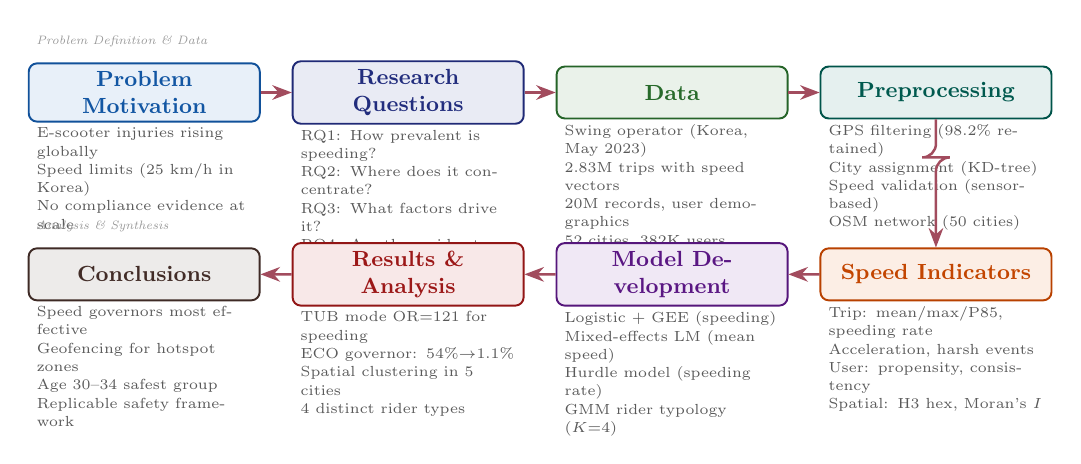
\begin{tikzpicture}[
    scale=0.88, every node/.style={transform shape},
    >=Stealth,
    stage/.style={
      rectangle, rounded corners=3pt,
      minimum width=3.3cm, minimum height=0.75cm,
      text width=3.1cm, align=center,
      font=\small\bfseries,
      draw=#1!80!black, fill=#1!10, text=#1!85!black,
      line width=0.7pt,
    },
    detail/.style={
      font=\fontsize{6}{7.5}\selectfont,
      text width=3.1cm, align=left, text=black!65,
      inner sep=0pt,
    },
    arrow/.style={->, umnmaroon!70, line width=0.9pt},
  ]

  \node[stage=boxblue] (motiv) {Problem Motivation};
  \node[detail, below=2pt of motiv] (motiv-d)
    {E-scooter injuries rising globally\\
     Speed limits (25 km/h in Korea)\\
     No compliance evidence at scale};

  \node[stage=boxindigo, right=0.45cm of motiv] (rq) {Research Questions};
  \node[detail, below=2pt of rq] (rq-d)
    {RQ1: How prevalent is speeding?\\
     RQ2: Where does it concentrate?\\
     RQ3: What factors drive it?\\
     RQ4: Are there rider typologies?};

  \node[stage=boxgreen, right=0.45cm of rq] (data) {Data};
  \node[detail, below=2pt of data] (data-d)
    {Swing operator (Korea, May 2023)\\
     2.83M trips with speed vectors\\
     20M records, user demographics\\
     52 cities, 382K users};

  \node[stage=boxteal, right=0.45cm of data] (preproc) {Preprocessing};
  \node[detail, below=2pt of preproc] (preproc-d)
    {GPS filtering (98.2\% retained)\\
     City assignment (KD-tree)\\
     Speed validation (sensor-based)\\
     OSM network (50 cities)};

  \draw[arrow] (motiv.east) -- (rq.west);
  \draw[arrow] (rq.east) -- (data.west);
  \draw[arrow] (data.east) -- (preproc.west);

  \node[stage=boxorange, below=1.85cm of preproc] (indicators) {Speed Indicators};
  \node[detail, below=2pt of indicators] (ind-d)
    {Trip: mean/max/P85, speeding rate\\
     Acceleration, harsh events\\
     User: propensity, consistency\\
     Spatial: H3 hex, Moran's $I$};

  \node[stage=boxpurple, left=0.45cm of indicators] (models) {Model Development};
  \node[detail, below=2pt of models] (mod-d)
    {Logistic + GEE (speeding)\\
     Mixed-effects LM (mean speed)\\
     Hurdle model (speeding rate)\\
     GMM rider typology ($K$=4)};

  \node[stage=boxred, left=0.45cm of models] (results) {Results \& Analysis};
  \node[detail, below=2pt of results] (res-d)
    {TUB mode OR=121 for speeding\\
     ECO governor: 54\%$\to$1.1\%\\
     Spatial clustering in 5 cities\\
     4 distinct rider types};

  \node[stage=boxbrown, left=0.45cm of results] (conclude) {Conclusions};
  \node[detail, below=2pt of conclude] (con-d)
    {Speed governors most effective\\
     Geofencing for hotspot zones\\
     Age 30--34 safest group\\
     Replicable safety framework};

  \draw[arrow, rounded corners=5pt]
    (preproc.south) -- ++(0,-0.55) -| (indicators.north);
  \draw[arrow] (indicators.west) -- (models.east);
  \draw[arrow] (models.west) -- (results.east);
  \draw[arrow] (results.west) -- (conclude.east);

  \node[font=\tiny\itshape, text=black!40, above=3pt of motiv.north west, anchor=south west]
    {Problem Definition \& Data};
  \node[font=\tiny\itshape, text=black!40, above=3pt of conclude.north west, anchor=south west]
    {Analysis \& Synthesis};
\end{tikzpicture}
\end{frame}

% ═══════════════════════════════════════════════════════════════════════════
% SLIDE 3: PROBLEM MOTIVATION
% ═══════════════════════════════════════════════════════════════════════════
\begin{frame}{Problem Motivation}
\begin{columns}[T]
\begin{column}{0.52\textwidth}
  \footnotesize
  \textbf{\textcolor{boxblue}{Global E-Scooter Safety Crisis}}
  \begin{itemize}\setlength\itemsep{1pt}
    \item E-scooter injuries increased \textbf{222\%} (2017--2021)
    \item Head injuries, fractures, fatalities in mixed traffic
    \item Pedestrian conflicts on sidewalks and shared paths
  \end{itemize}

  \vspace{4pt}
  \textbf{\textcolor{boxblue}{Regulatory Response}}
  \begin{itemize}\setlength\itemsep{1pt}
    \item Korea: \textbf{25 km/h} limit (Road Traffic Act, 2021)
    \item Germany: 20 km/h; France: 25 km/h; US cities: 15--25 mph
    \item Operators deploy speed governors (ECO, STD, TUB modes)
  \end{itemize}

  \vspace{4pt}
  \textbf{\textcolor{boxblue}{Knowledge Gap}}
  \begin{itemize}\setlength\itemsep{1pt}
    \item No large-scale evidence on \textbf{actual compliance}
    \item Prior studies: small samples ($n < 1{,}000$), single-city, survey-based
    \item No within-trip speed dynamics at population scale
  \end{itemize}
\end{column}
\begin{column}{0.45\textwidth}
  \centering
  \vspace{4pt}
  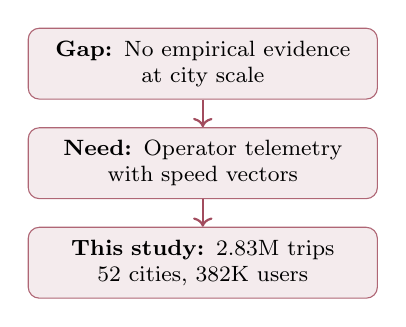
\begin{tikzpicture}[
    box/.style={rectangle, rounded corners=4pt, draw=umnmaroon!60, fill=umnmaroon!8,
                text width=4.2cm, minimum height=0.9cm, align=center, font=\footnotesize},
    arr/.style={->, umnmaroon!70, line width=0.8pt},
  ]
    \node[box] (gap) {\textbf{Gap:} No empirical evidence\\at city scale};
    \node[box, below=0.35cm of gap] (need) {\textbf{Need:} Operator telemetry\\with speed vectors};
    \node[box, below=0.35cm of need] (our) {\textbf{This study:} 2.83M trips\\52 cities, 382K users};
    \draw[arr] (gap) -- (need);
    \draw[arr] (need) -- (our);
  \end{tikzpicture}

  \vspace{10pt}
  \footnotesize
  \textbf{Target:} Transportation Research Part C\\
  \textbf{Scope:} First city-scale e-scooter speed study with full within-trip speed profiles
\end{column}
\end{columns}
\end{frame}

% ═══════════════════════════════════════════════════════════════════════════
% SLIDE 4: RESEARCH QUESTIONS
% ═══════════════════════════════════════════════════════════════════════════
\begin{frame}{Research Questions}
\footnotesize
\begin{description}[\textbf{RQ4}]
  \item[\textcolor{boxindigo}{\textbf{RQ1}}] \textbf{Speed Prevalence} ---
    What are the distributional characteristics of e-scooter riding speed at the trip and within-trip levels, and how prevalent is speeding ($>$25 km/h) across a city-scale dataset?
    \vspace{4pt}

  \item[\textcolor{boxindigo}{\textbf{RQ2}}] \textbf{Spatial Concentration} ---
    Where do spatially concentrated speed-related safety risks occur, and what road infrastructure attributes are associated with elevated speeding?
    \vspace{4pt}

  \item[\textcolor{boxindigo}{\textbf{RQ3}}] \textbf{Contributing Factors} ---
    How do rider demographics (age), vehicle characteristics (model, mode), and temporal factors influence speed behavior and speeding propensity?
    \vspace{4pt}

  \item[\textcolor{boxindigo}{\textbf{RQ4}}] \textbf{Rider Typologies} ---
    Can we identify distinct rider speed behavior typologies, and how do these distribute across cities and demographic groups?
\end{description}

\vspace{8pt}
\centering
\hlbox{boxindigo}{RQ1: Descriptive} \quad
\hlbox{boxgreen}{RQ2: Spatial} \quad
\hlbox{boxorange}{RQ3: Regression} \quad
\hlbox{boxpurple}{RQ4: Clustering}
\end{frame}

% ═══════════════════════════════════════════════════════════════════════════
% SLIDE 5: DATA — Scale & Coverage
% ═══════════════════════════════════════════════════════════════════════════
\begin{frame}{Data: Scale \& Spatial Coverage}
\begin{columns}[T]
\begin{column}{0.43\textwidth}
  \footnotesize
  \textbf{\textcolor{boxgreen}{Swing Operator Data (Korea)}}
  \vspace{2pt}

  \begin{tabular}{@{}l r@{}}
    \toprule
    \textbf{Attribute} & \textbf{Value} \\
    \midrule
    Trajectory dataset & May 2023 \\
    Total trips & 2,830,461 \\
    After filtering & 2,780,890 \\
    Unique users & 382,328 \\
    Unique vehicles & 81,525 \\
    Cities covered & 52 \\
    Provinces & 17 \\
    \midrule
    Trip-level dataset & Jan--Oct 2023 \\
    Total records & 20M \\
    Users with age data & 90.4\% \\
    Median user age & 25 years \\
    \bottomrule
  \end{tabular}

  \vspace{4pt}
  \textbf{Key:} Per-trip \texttt{speeds} vector at ${\sim}$10s intervals enables within-trip speed dynamics
\end{column}
\begin{column}{0.55\textwidth}
  \centering
  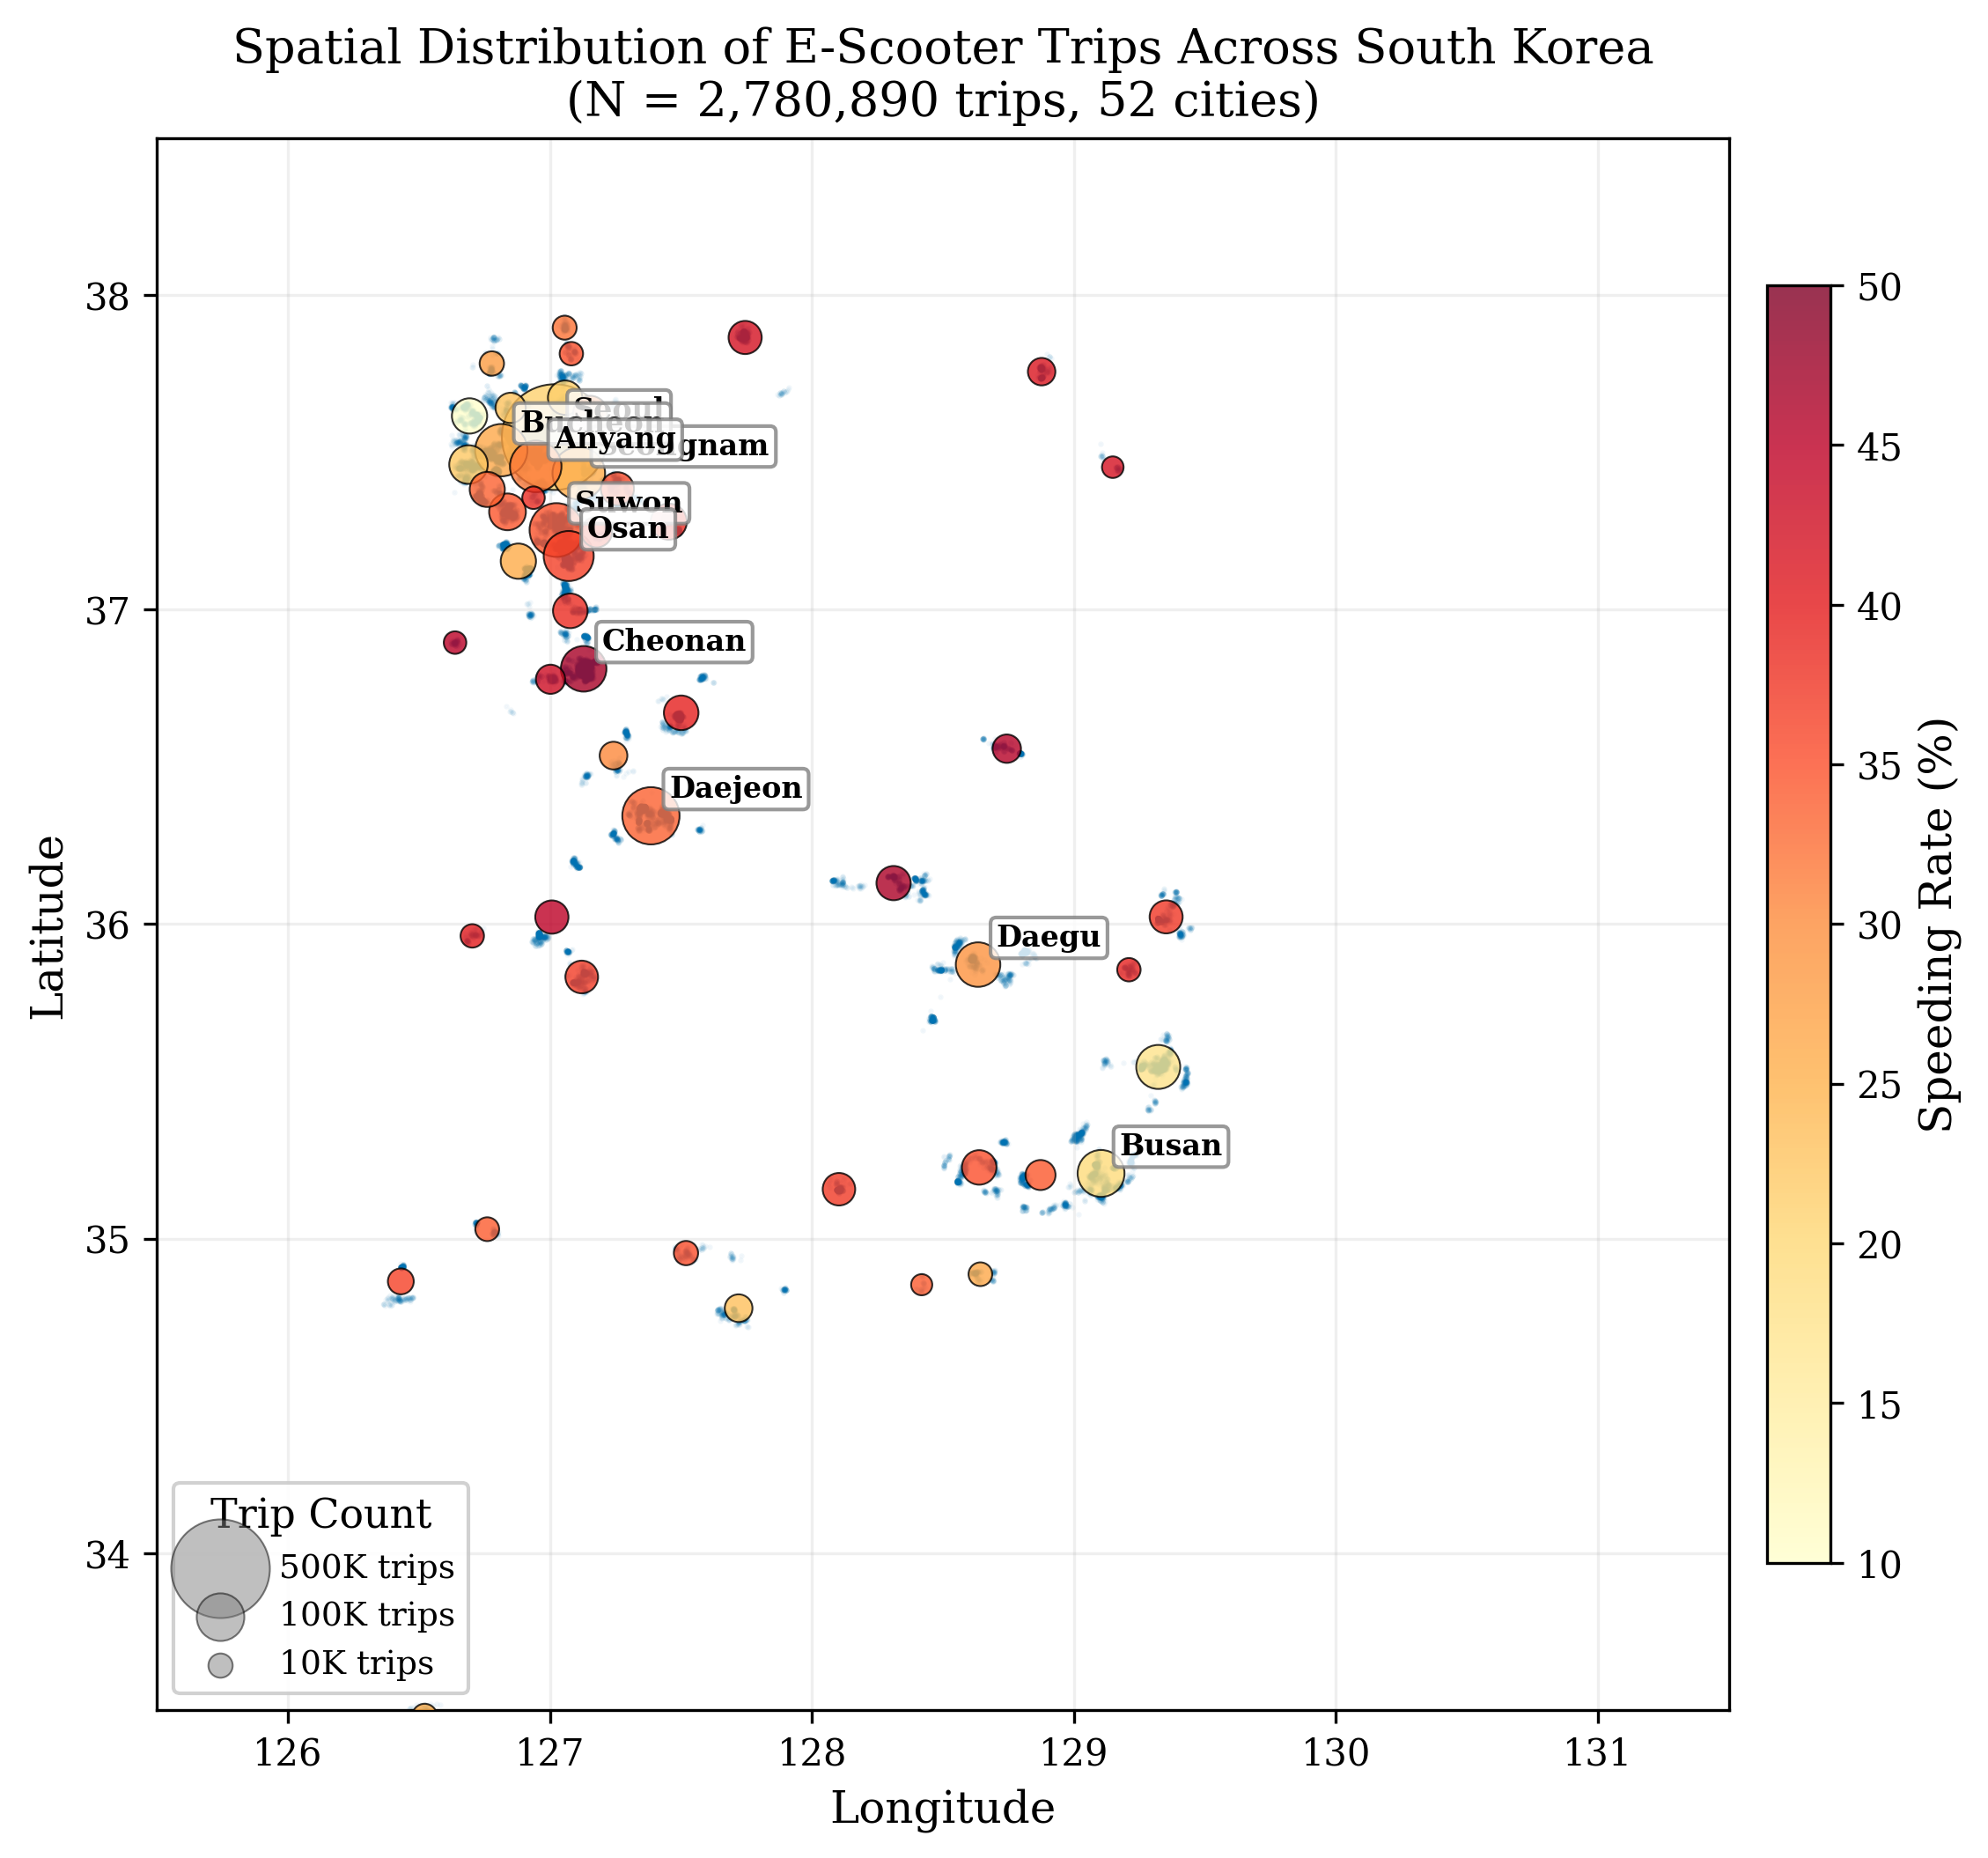
\includegraphics[width=\linewidth,height=0.72\textheight,keepaspectratio]{fig1_spatial_distribution.png}
  \vspace{-6pt}

  {\scriptsize Bubble size $=$ trip count; color $=$ speeding rate (\%).}
\end{column}
\end{columns}
\end{frame}

% ═══════════════════════════════════════════════════════════════════════════
% SLIDE 6: DATA — Temporal Patterns & Speed Profiles
% ═══════════════════════════════════════════════════════════════════════════
\begin{frame}{Data: Temporal Patterns \& Speed Profiles}
\begin{columns}[T]
\begin{column}{0.55\textwidth}
  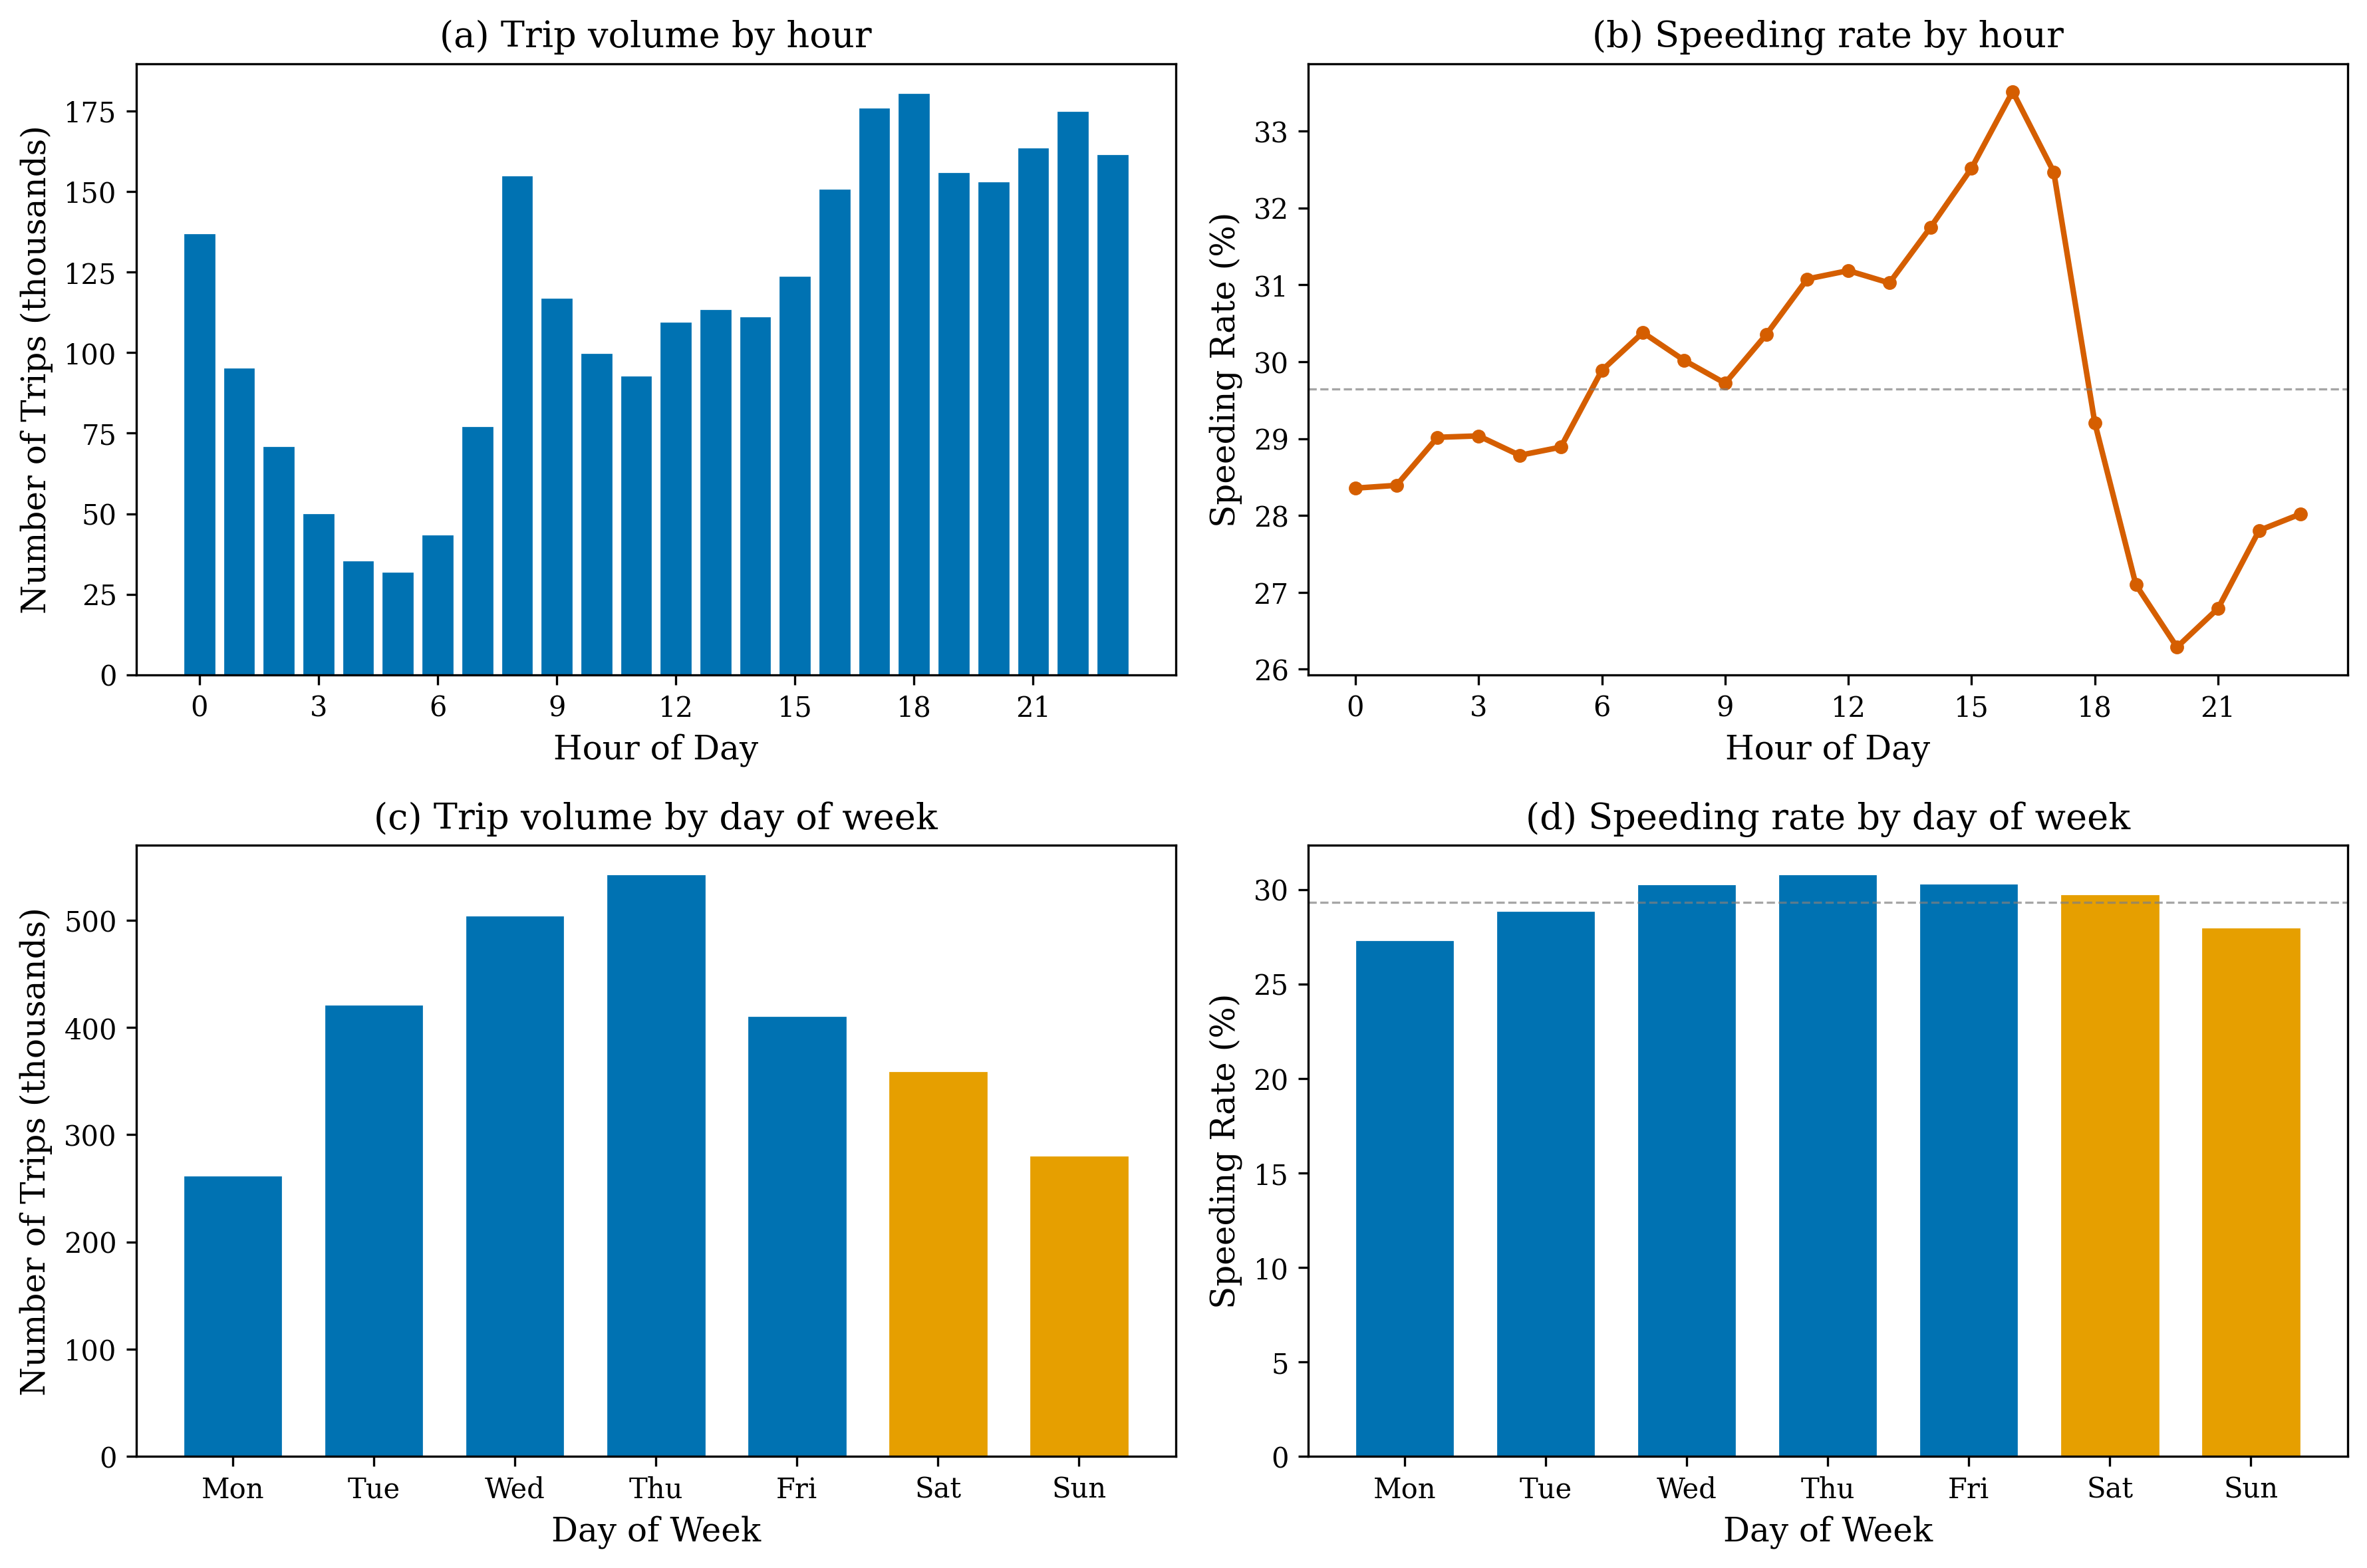
\includegraphics[width=\linewidth]{fig2_temporal_distributions.png}
  \vspace{-4pt}

  {\scriptsize (a,c) Trip volume peaks at 18:00 and Thu--Fri. (b,d) Speeding rate peaks 14:00--16:00 (35\%); stable across days.}
\end{column}
\begin{column}{0.43\textwidth}
  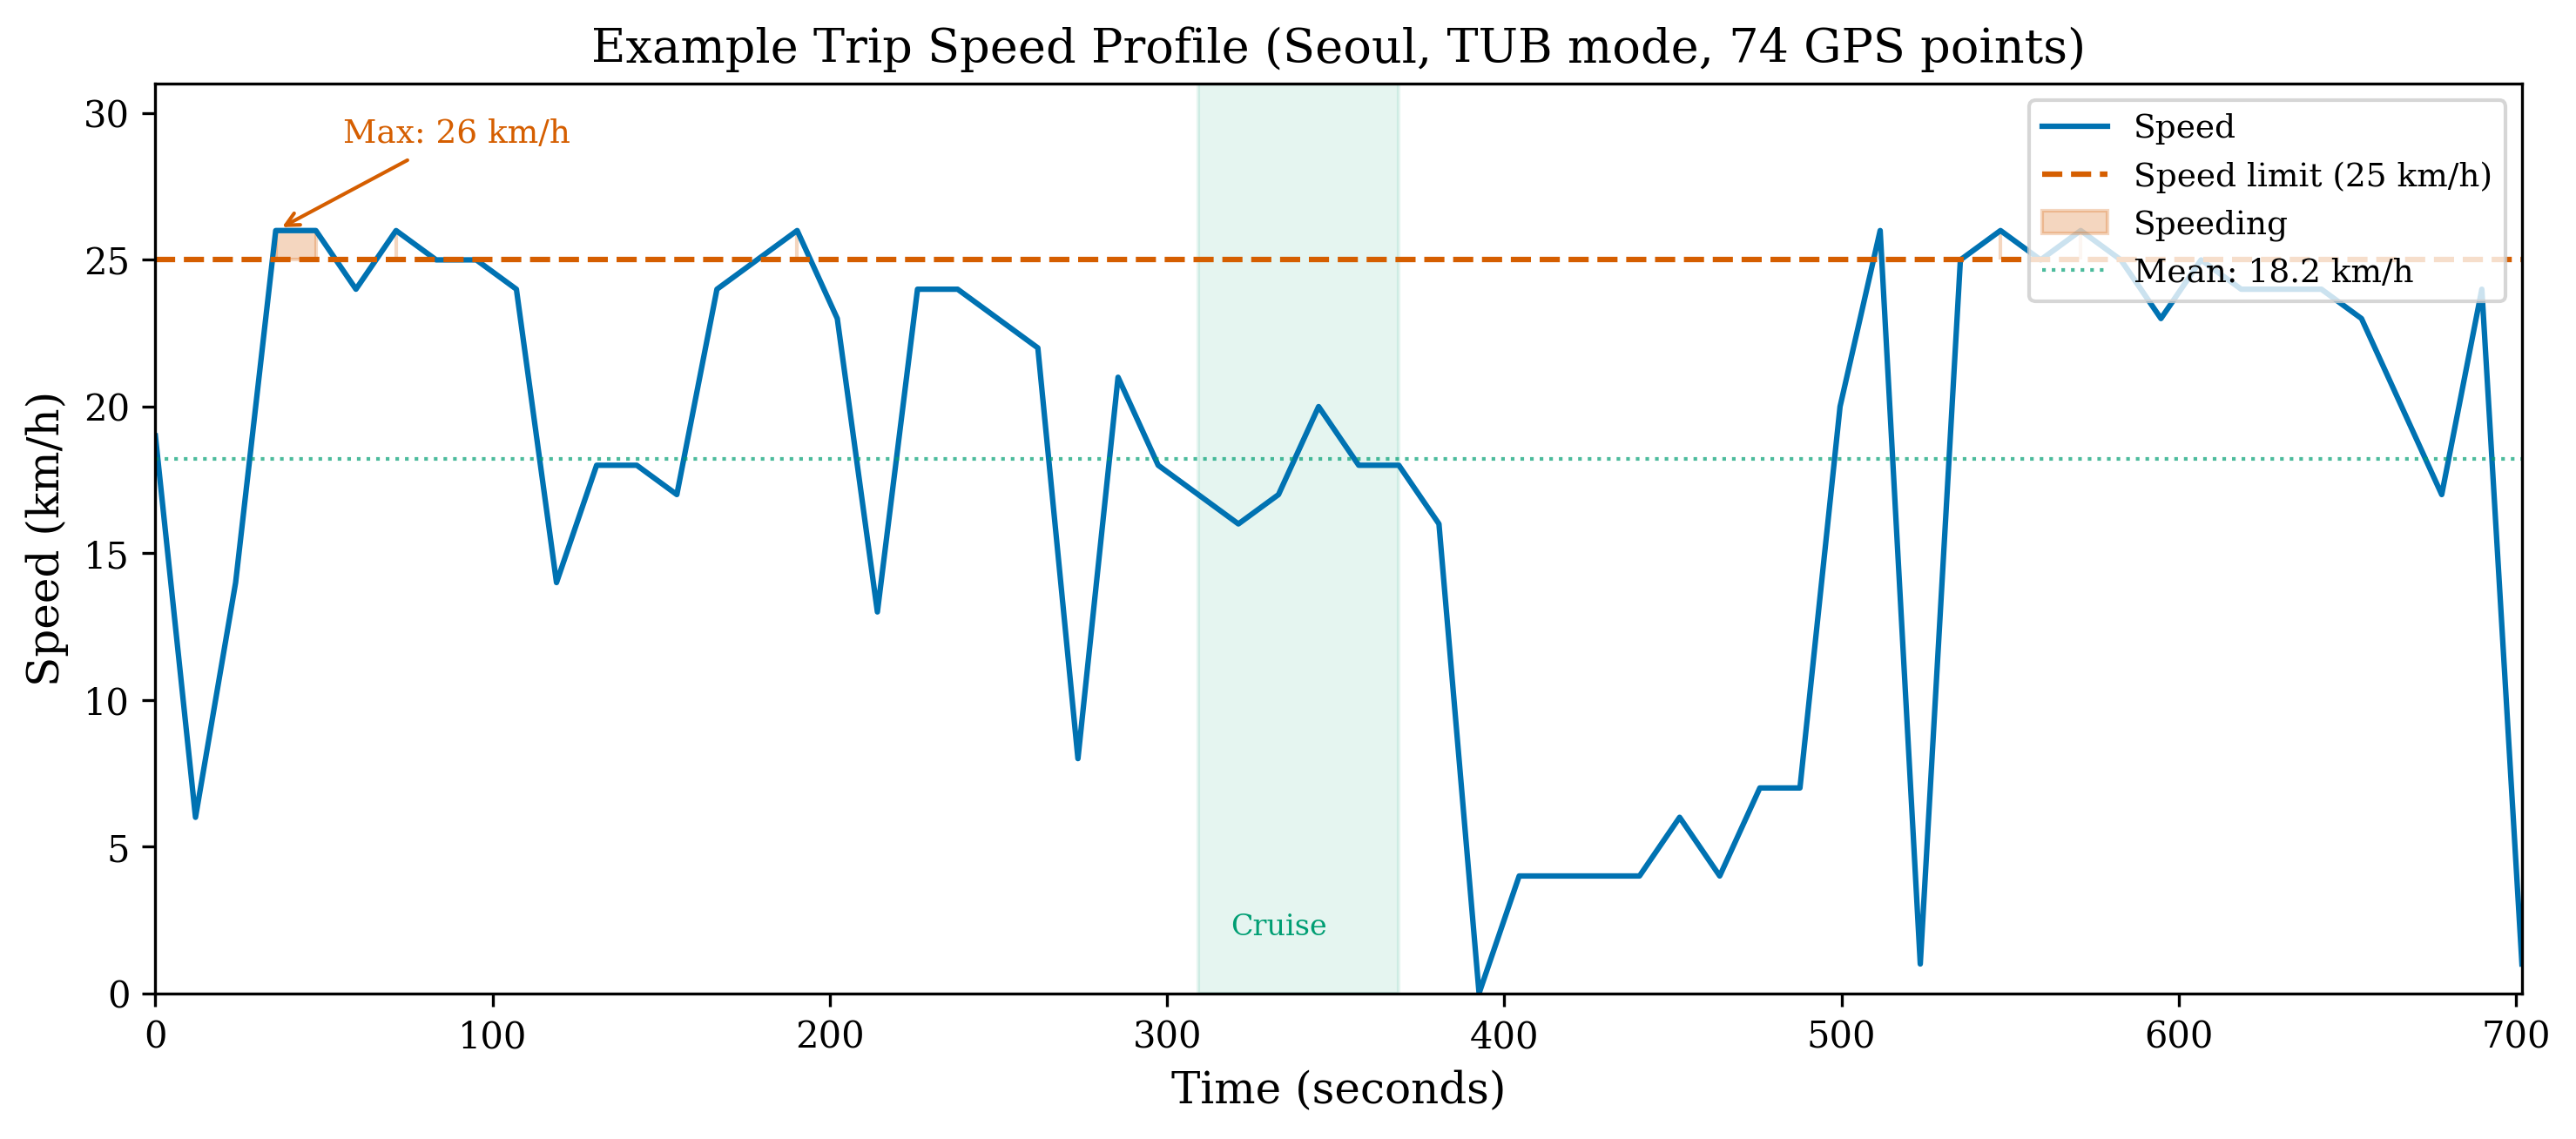
\includegraphics[width=\linewidth]{fig3_speed_profile_example.png}
  \vspace{-4pt}

  {\scriptsize Example trip: Seoul, TUB mode, 74 GPS points. Dashed $=$ 25 km/h limit. Shaded $=$ speeding episodes.}

  \vspace{4pt}
  \footnotesize
  \textbf{\textcolor{boxgreen}{Speed Vector Properties}}
  \begin{itemize}\setlength\itemsep{1pt}
    \item Sensor-based (not GPS-derived)
    \item $r = 1.0$ with reported \texttt{max\_speed}
    \item 10-second average intervals
    \item Enables acceleration, cruise fraction, harsh event computation
  \end{itemize}
\end{column}
\end{columns}
\end{frame}

% ═══════════════════════════════════════════════════════════════════════════
% SLIDE 7: PREPROCESSING PIPELINE
% ═══════════════════════════════════════════════════════════════════════════
\begin{frame}{Preprocessing Pipeline}
\vspace{-4pt}
\centering
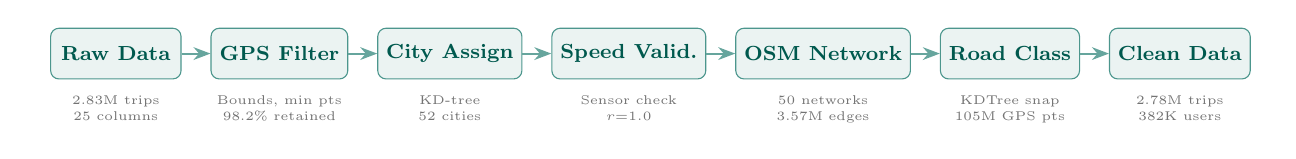
\begin{tikzpicture}[
    scale=0.92, every node/.style={transform shape},
    >=Stealth,
    box/.style={rectangle, rounded corners=3pt, draw=boxteal!70, fill=boxteal!8,
                minimum width=1.8cm, minimum height=0.7cm, align=center,
                font=\footnotesize\bfseries, text=boxteal!85!black},
    stat/.style={font=\tiny, text=black!55, align=center, text width=2.2cm},
    arr/.style={->, boxteal!60, line width=0.7pt},
  ]
  \node[box] (raw) {Raw Data};
  \node[box, right=0.4cm of raw] (gps) {GPS Filter};
  \node[box, right=0.4cm of gps] (city) {City Assign};
  \node[box, right=0.4cm of city] (speed) {Speed Valid.};
  \node[box, right=0.4cm of speed] (osm) {OSM Network};
  \node[box, right=0.4cm of osm] (road) {Road Class};
  \node[box, right=0.4cm of road] (clean) {Clean Data};

  \draw[arr] (raw) -- (gps);
  \draw[arr] (gps) -- (city);
  \draw[arr] (city) -- (speed);
  \draw[arr] (speed) -- (osm);
  \draw[arr] (osm) -- (road);
  \draw[arr] (road) -- (clean);

  \node[stat, below=3pt of raw] {2.83M trips\\25 columns};
  \node[stat, below=3pt of gps] {Bounds, min pts\\98.2\% retained};
  \node[stat, below=3pt of city] {KD-tree\\52 cities};
  \node[stat, below=3pt of speed] {Sensor check\\$r{=}1.0$};
  \node[stat, below=3pt of osm] {50 networks\\3.57M edges};
  \node[stat, below=3pt of road] {KDTree snap\\105M GPS pts};
  \node[stat, below=3pt of clean] {2.78M trips\\382K users};
\end{tikzpicture}

\vspace{6pt}
\begin{columns}[T]
\begin{column}{0.48\textwidth}
  \footnotesize
  \textbf{GPS Filtering Criteria}
  \begin{itemize}\setlength\itemsep{1pt}
    \item Korean bounds: lat $[33, 39]$, lon $[124, 132]$
    \item Min 5 GPS points, distance $> 100$m, duration $> 60$s
    \item Remove sentinel $-999$ in 6 numeric columns
    \item Result: 2,780,890 valid trips (\textbf{98.2\%} retention)
  \end{itemize}
\end{column}
\begin{column}{0.48\textwidth}
  \footnotesize
  \textbf{OSM Road Network \& Road Class Assignment}
  \begin{itemize}\setlength\itemsep{1pt}
    \item 50 cities via \texttt{osmnx} 2.0.7 (1.32M nodes, 3.57M edges)
    \item Road class from \texttt{highway} tag (100\% coverage)
    \item DuckDB + scipy KDTree: 105M GPS points in 463s
    \item Dominant: residential 41\%, tertiary 15\%, service 15\%
  \end{itemize}
\end{column}
\end{columns}
\end{frame}

% ═══════════════════════════════════════════════════════════════════════════
% SLIDE 8: SPEED INDICATORS — Framework
% ═══════════════════════════════════════════════════════════════════════════
\begin{frame}{Speed Indicators: Multi-Level Framework}
\vspace{-4pt}
\begin{columns}[T]
\begin{column}{0.52\textwidth}
  \footnotesize
  \textbf{\textcolor{boxorange}{Trip-Level Indicators}}
  \begin{itemize}\setlength\itemsep{0pt}
    \item Mean speed, max speed, P85 speed
    \item \textbf{Speeding rate}: fraction of observations $> 25$ km/h
    \item Speed CV (coefficient of variation)
    \item Cruise fraction, zero-speed fraction
    \item Harsh accel/decel: $|a| > 0.5$ m/s$^2$ (10s intervals)
  \end{itemize}

  \vspace{3pt}
  \textbf{\textcolor{boxorange}{User-Level Indicators}}
  \begin{itemize}\setlength\itemsep{0pt}
    \item Speeding propensity: frac.\ of trips with any speeding
    \item Aggregated trip-level means, speed consistency (variance)
  \end{itemize}

  \vspace{3pt}
  \textbf{\textcolor{boxorange}{Spatial Indicators}}
  \begin{itemize}\setlength\itemsep{0pt}
    \item H3 hex grid (res.\ 8, ${\sim}$460m edge), 8,144 hexes
    \item Per-hex speeding rate, road class composition
    \item Getis-Ord Gi* hotspots, Global/Local Moran's $I$
  \end{itemize}
\end{column}
\begin{column}{0.46\textwidth}
  \centering
  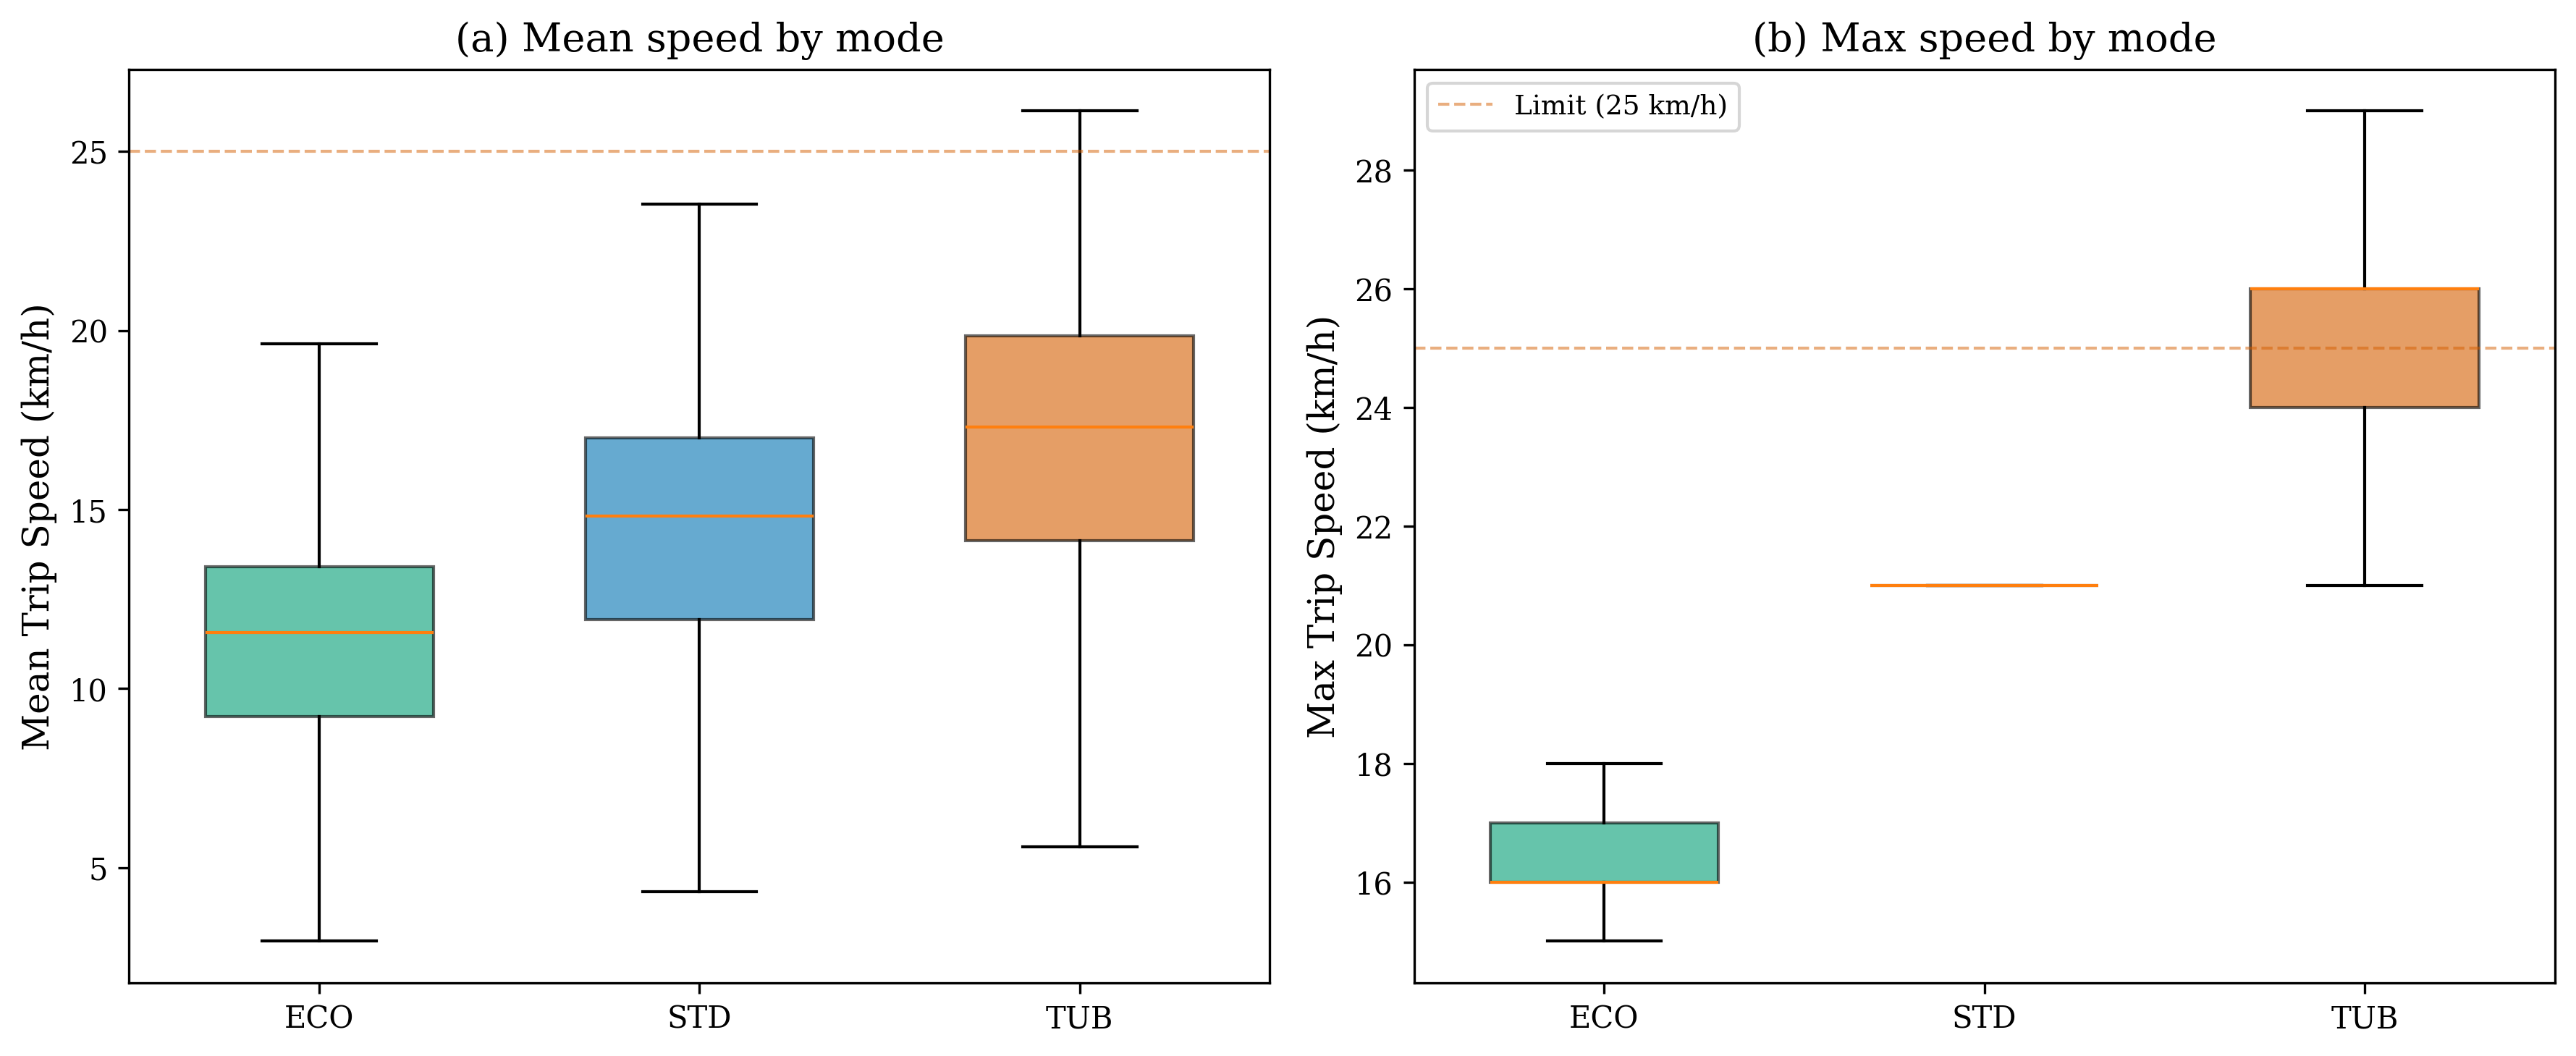
\includegraphics[width=\linewidth]{fig4_speed_by_mode.png}
  \vspace{-4pt}

  {\scriptsize Speed by operating mode. Dashed $=$ 25 km/h limit. TUB max speed extends well above limit; ECO capped below 18 km/h.}

  \vspace{3pt}
  \scriptsize
  \begin{tabular}{@{}l c c c@{}}
    \toprule
    \textbf{Mode} & \textbf{Mean} & \textbf{Max} & \textbf{Speeding} \\
    \midrule
    ECO & 11.5 & 16.5 & 1.1\% \\
    STD & 14.7 & 21.0 & 3.5\% \\
    TUB & 17.3 & 25.3 & 54.0\% \\
    \bottomrule
  \end{tabular}
\end{column}
\end{columns}
\end{frame}

% ═══════════════════════════════════════════════════════════════════════════
% SLIDE 9: SPEED INDICATORS — Speeding Prevalence
% ═══════════════════════════════════════════════════════════════════════════
\begin{frame}{Speed Indicators: Speeding Prevalence}
\begin{columns}[T]
\begin{column}{0.38\textwidth}
  \centering
  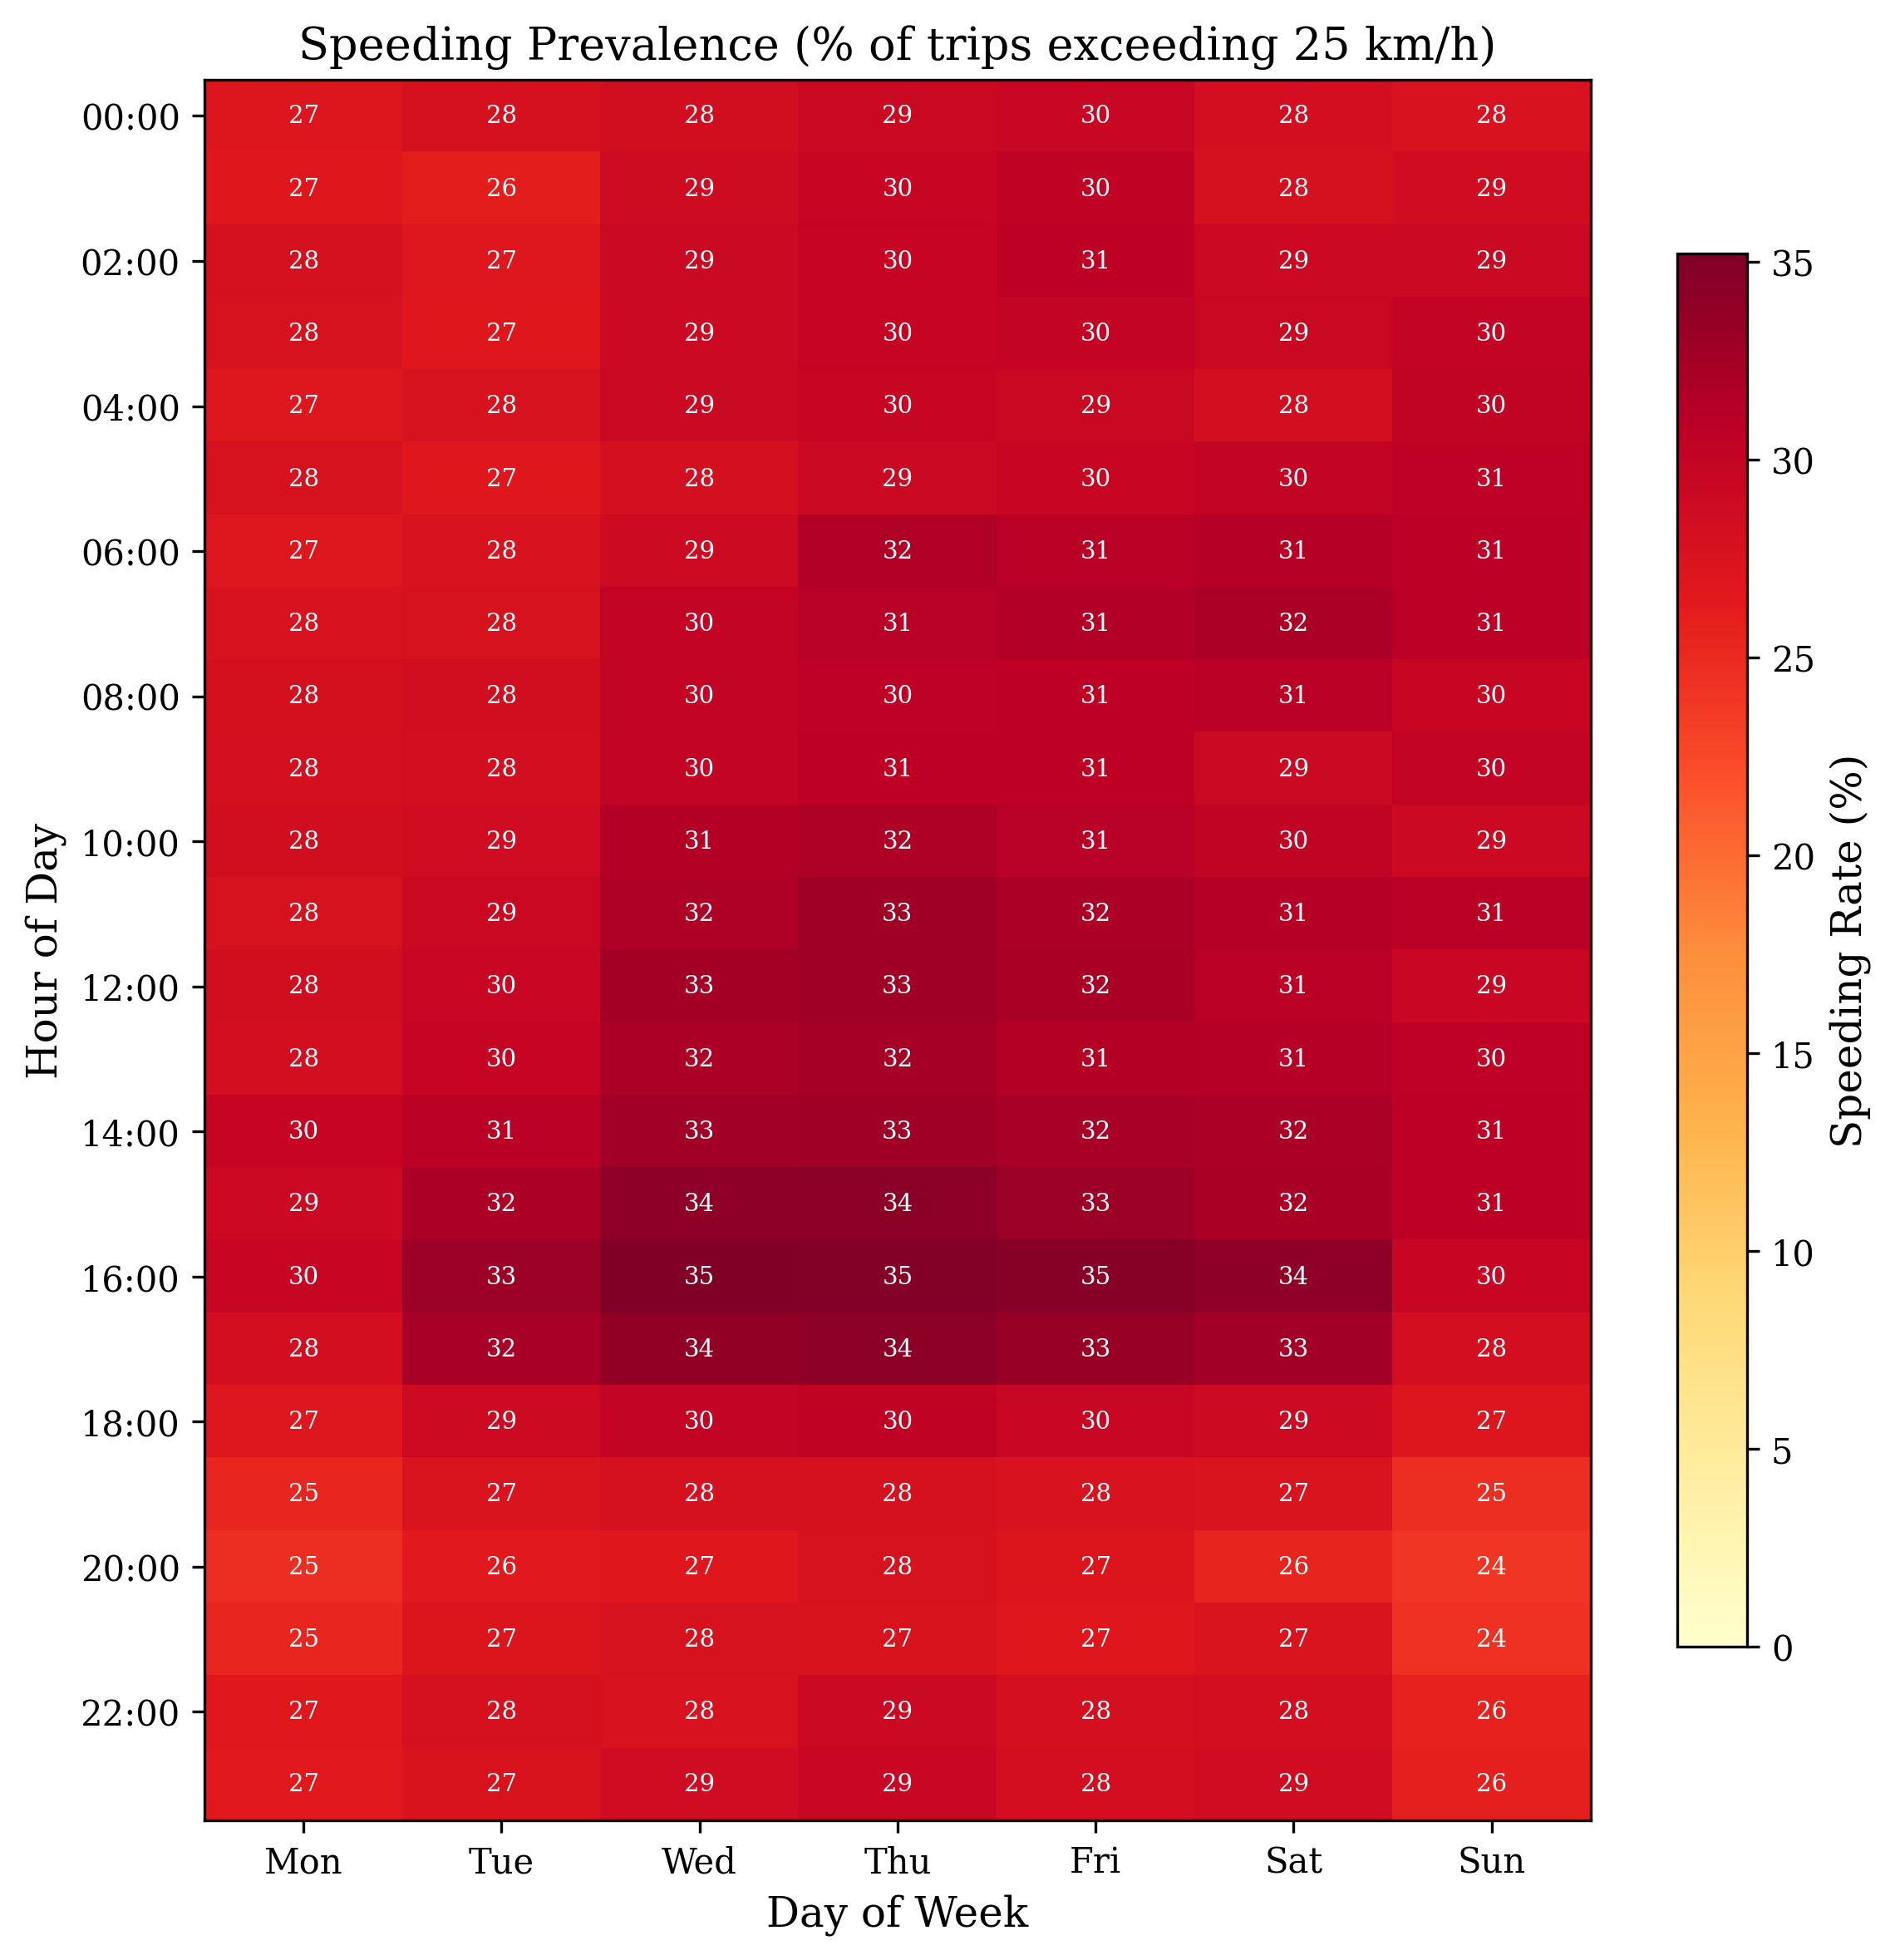
\includegraphics[width=\linewidth,height=0.62\textheight,keepaspectratio]{fig5_speeding_heatmap.png}
  \vspace{-4pt}

  {\scriptsize Speeding (\%) by hour $\times$ day. Peak: Thu 16:00 (35\%).}
\end{column}
\begin{column}{0.60\textwidth}
  \centering
  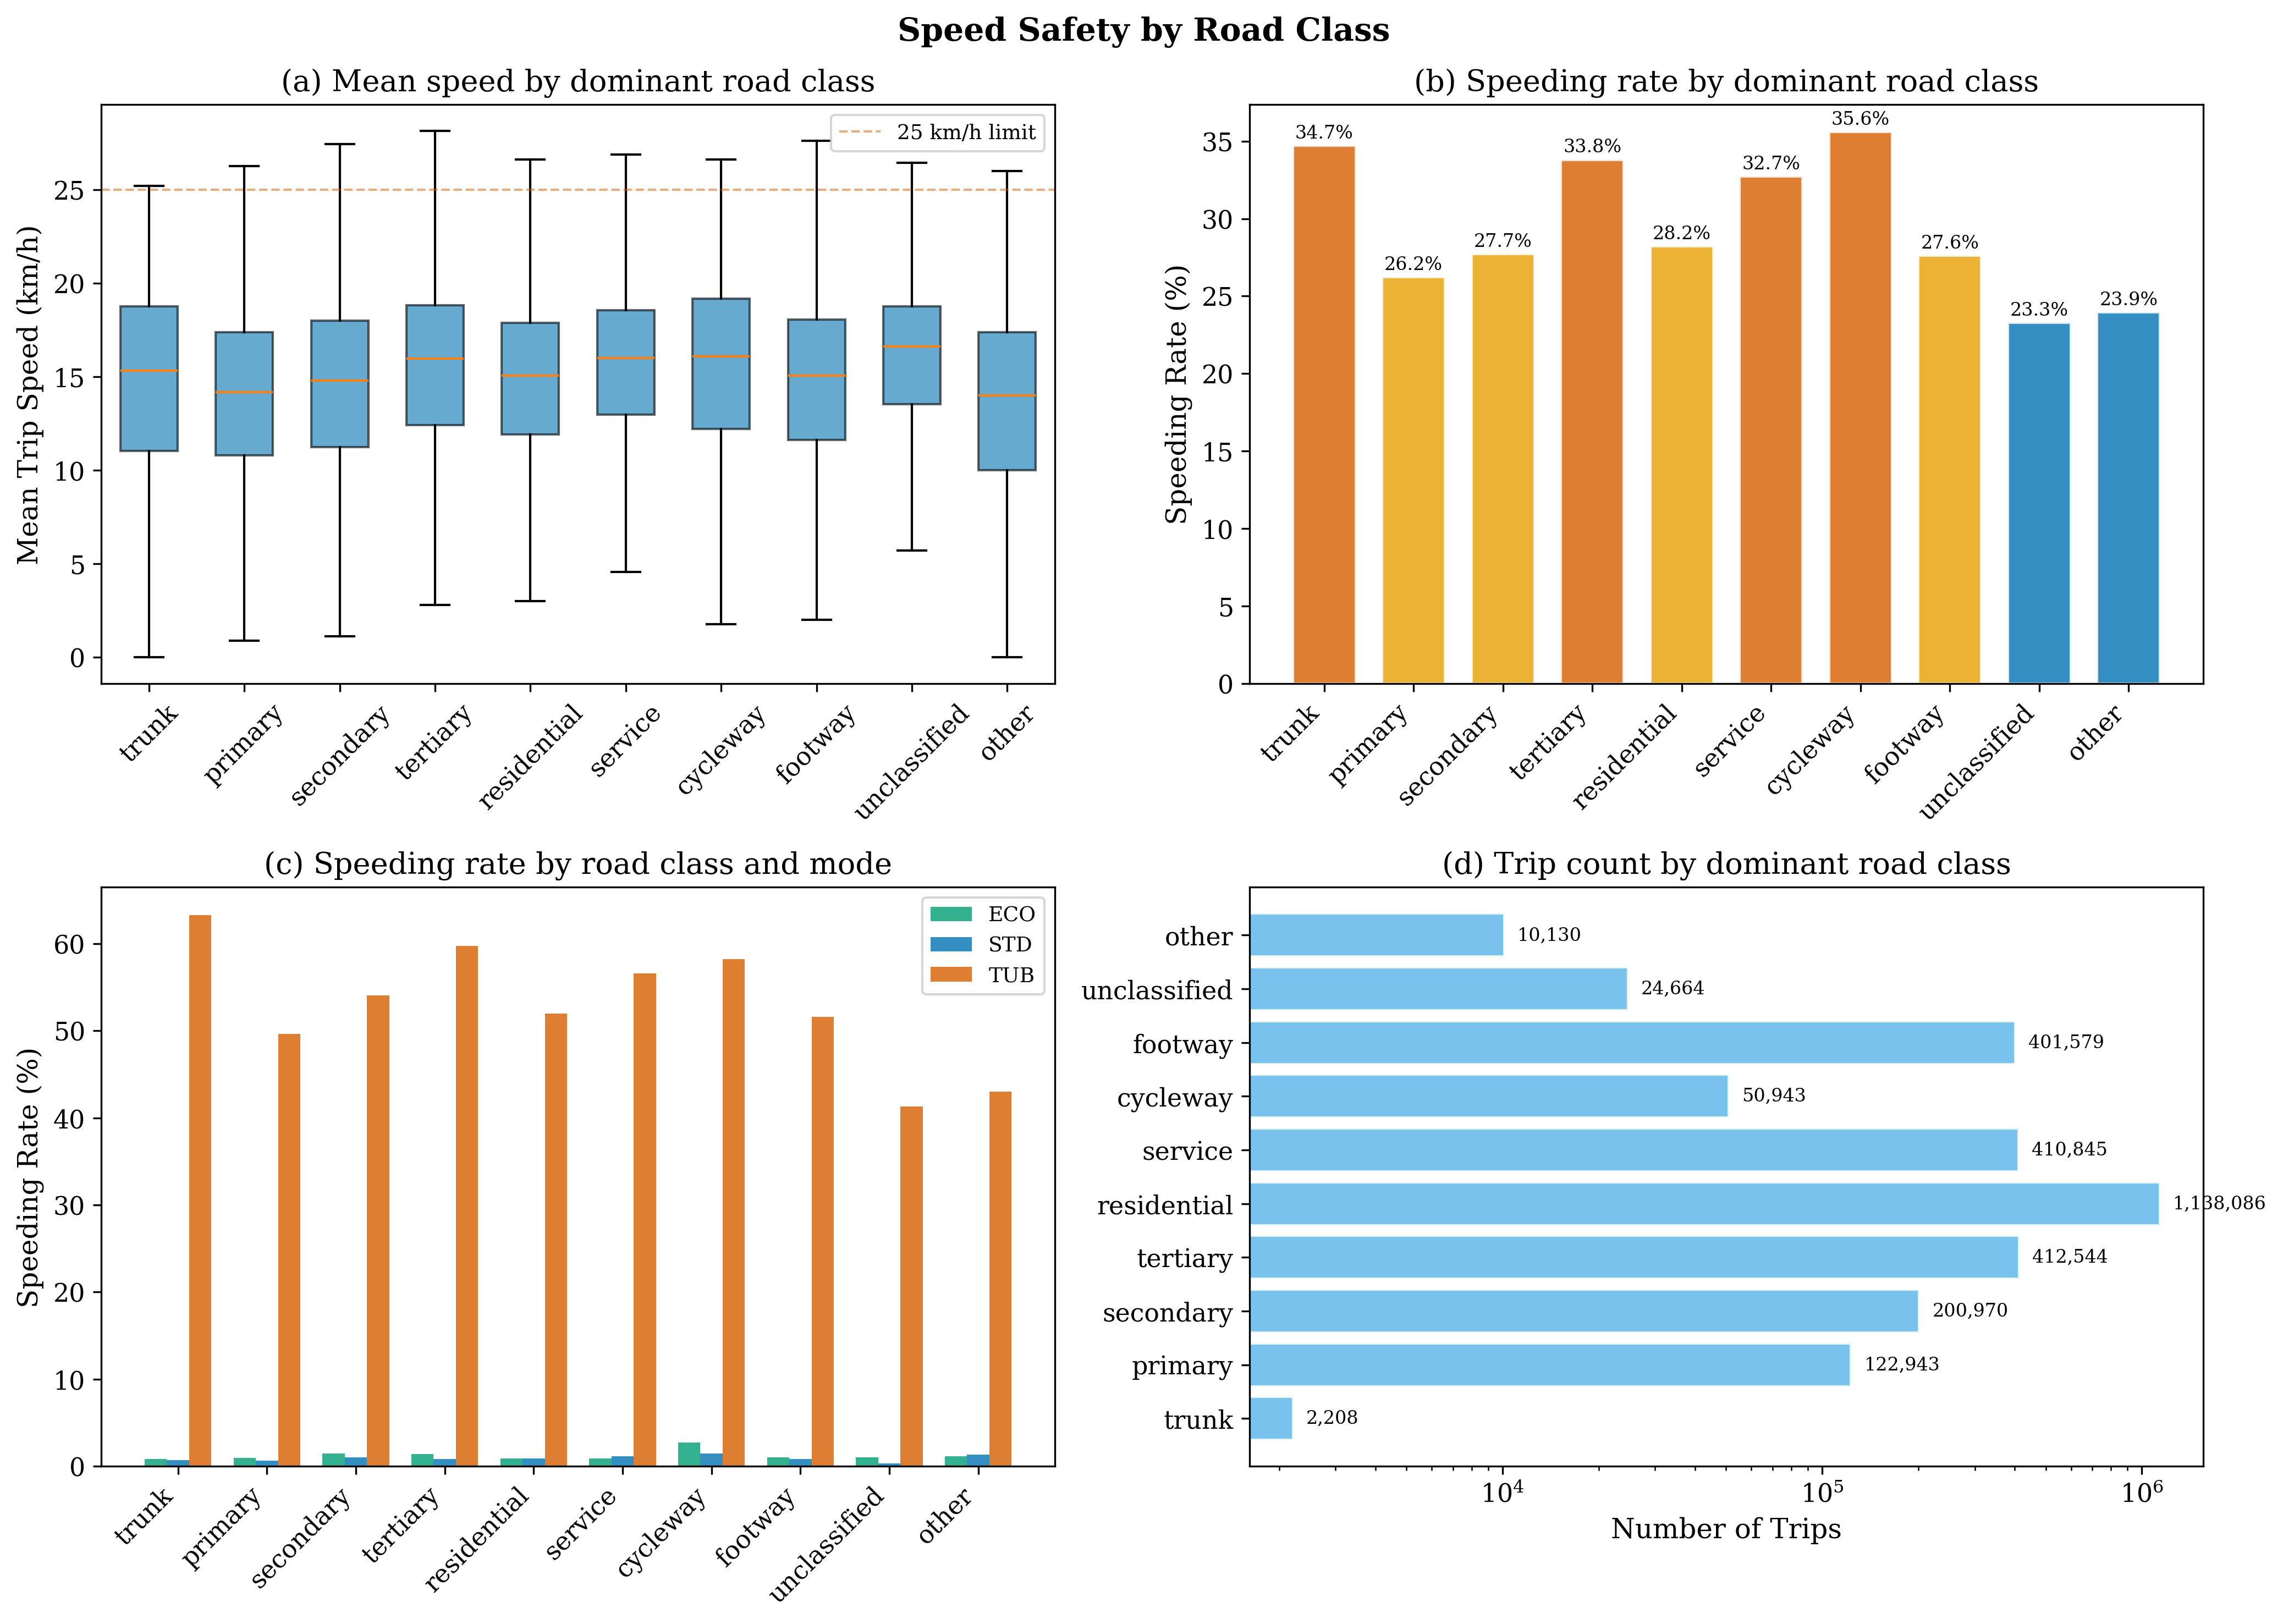
\includegraphics[width=\linewidth,height=0.62\textheight,keepaspectratio]{fig8_speed_by_road_class.png}
  \vspace{-4pt}

  {\scriptsize (a) Mean speed, (b) speeding rate by road class: trunk 34.7\%, footway 23\%, (c) by mode, (d) trip volume.}
\end{column}
\end{columns}

\vspace{4pt}
\centering
\hlbox{boxred}{29.6\% of trips exceed 25 km/h} \quad
\hlbox{boxorange}{60.9\% of users never speed} \quad
\hlbox{boxpurple}{17.3\% speed on $>$50\% of trips}
\end{frame}

% ═══════════════════════════════════════════════════════════════════════════
% SLIDE 10: SPATIAL ANALYSIS — Hotspot Detection
% ═══════════════════════════════════════════════════════════════════════════
\begin{frame}{Spatial Analysis: Hotspot Detection}
\begin{columns}[T]
\begin{column}{0.49\textwidth}
  \centering
  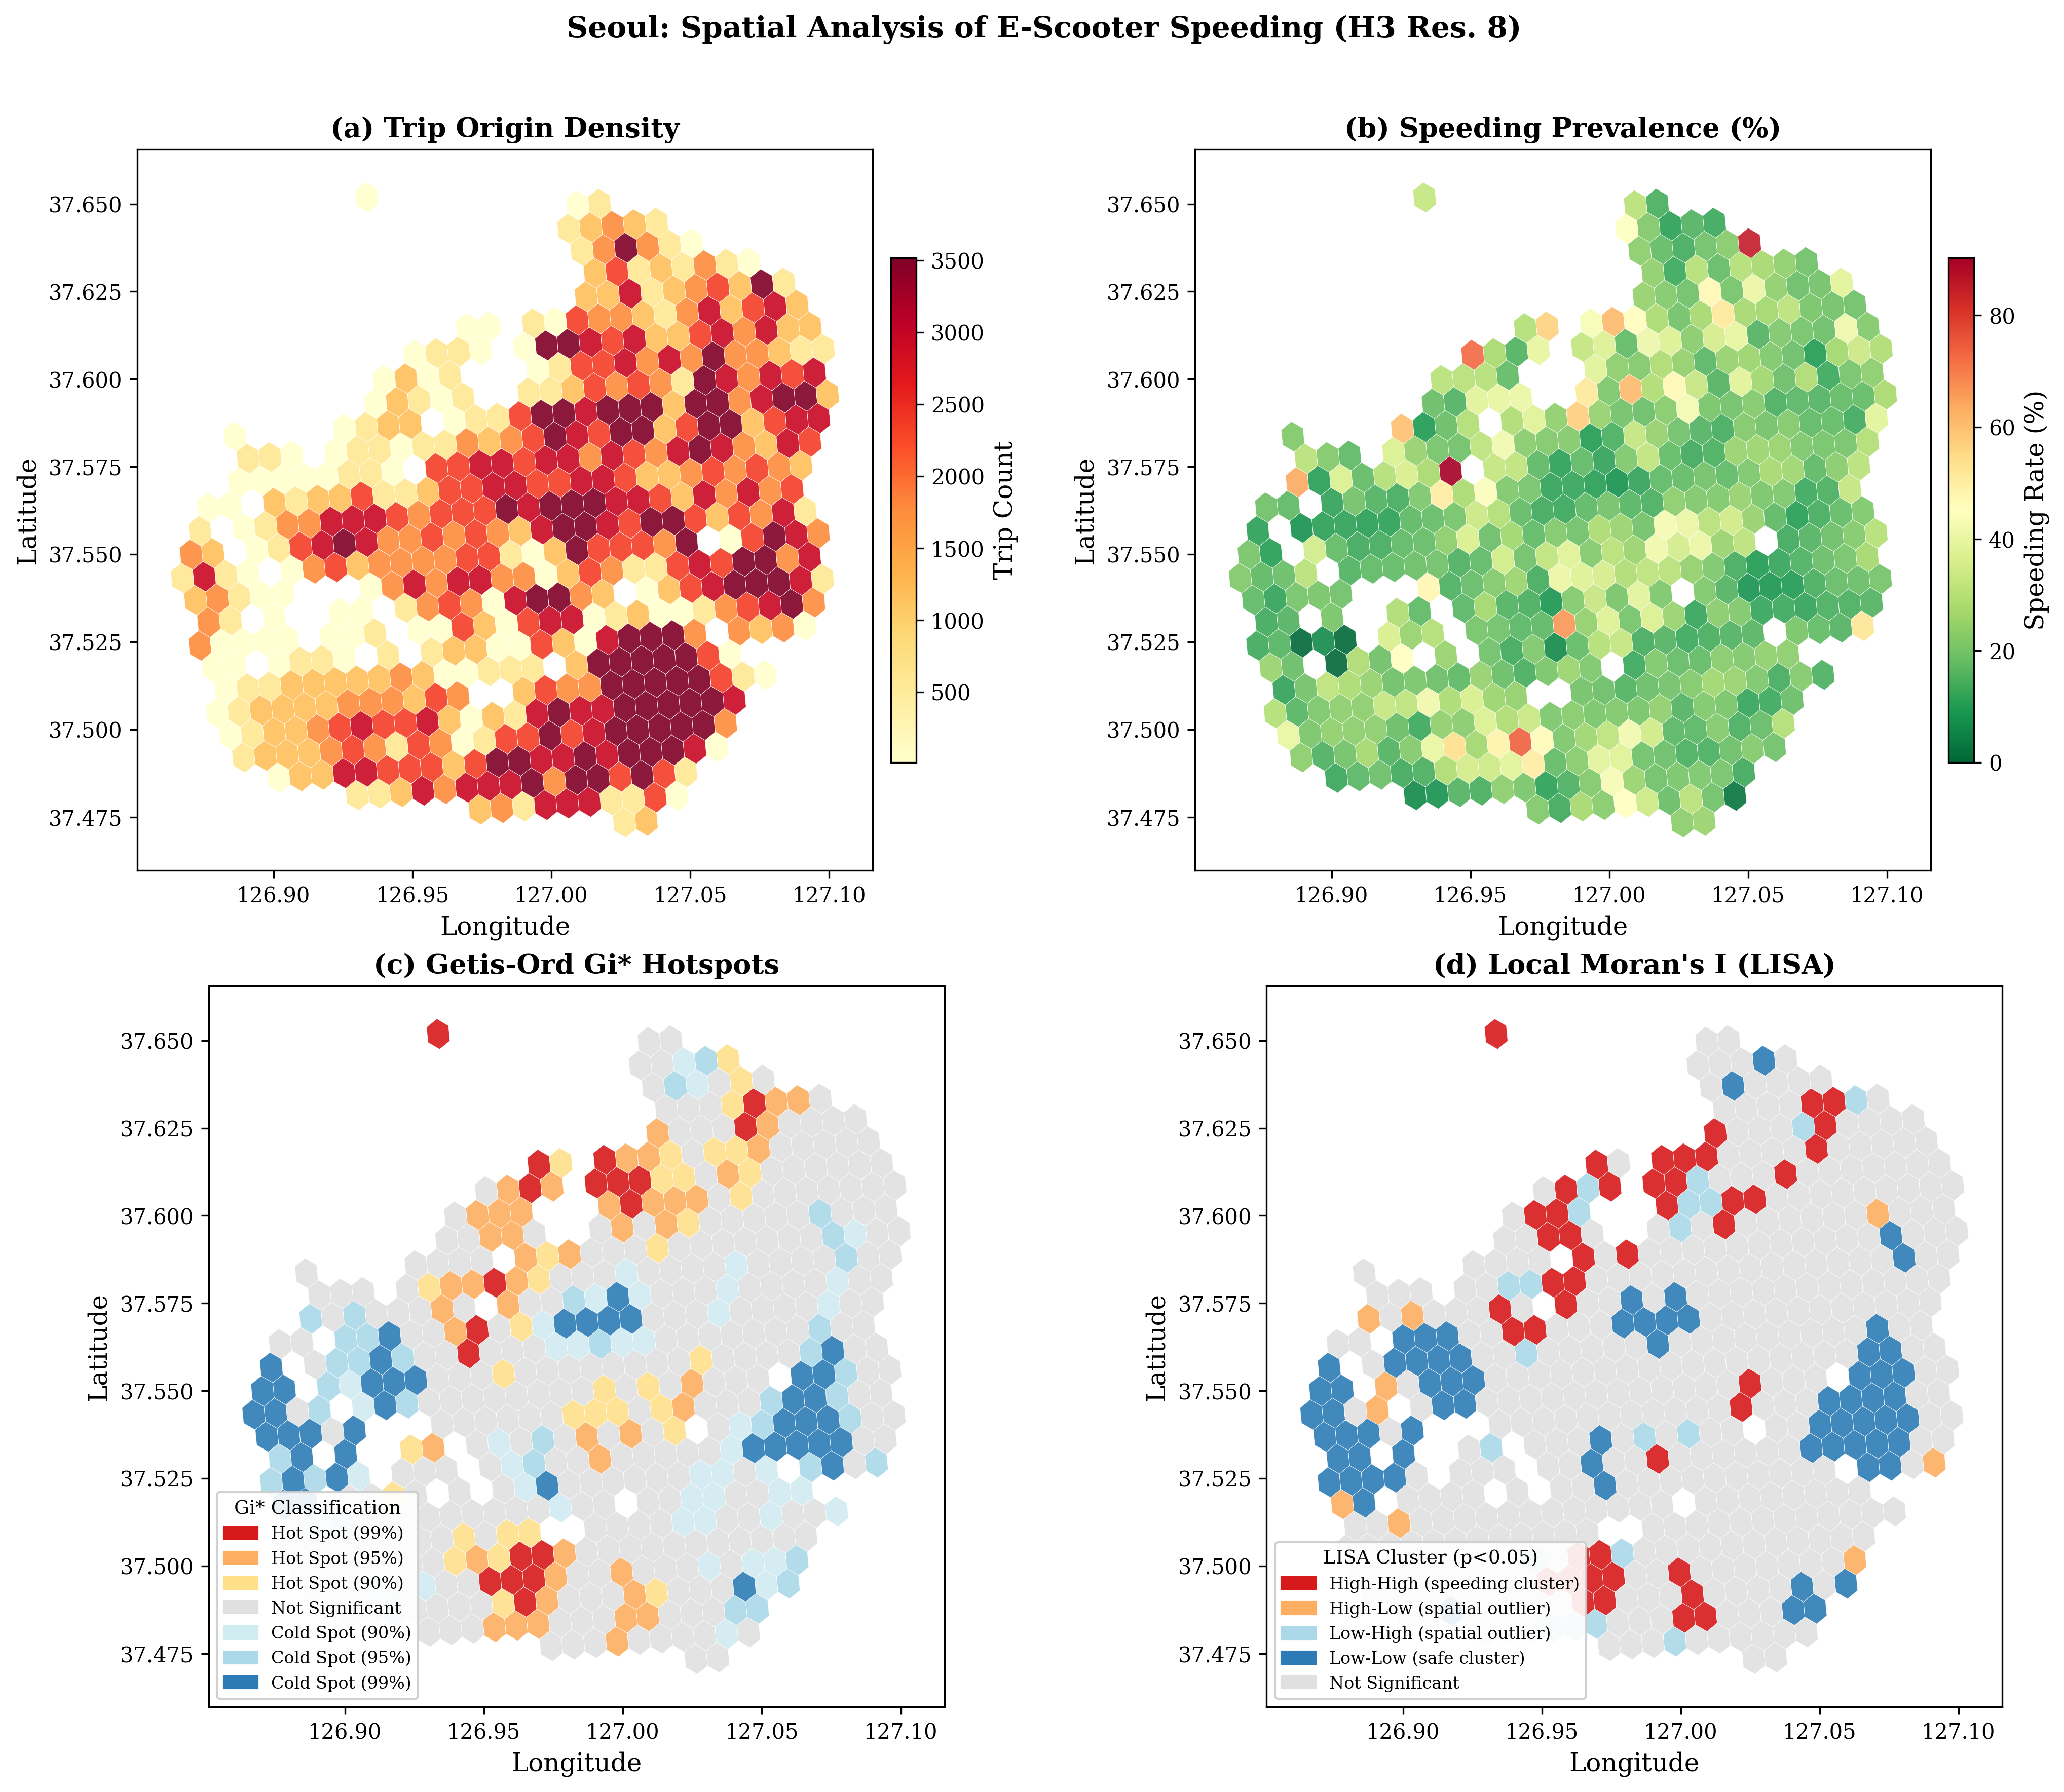
\includegraphics[width=\linewidth,height=0.52\textheight,keepaspectratio]{fig6_seoul_hotspot.png}
  \vspace{-4pt}

  {\scriptsize Seoul: (a) density, (b) speeding, (c) Gi* hotspots, (d) LISA. 101 hot / 123 cold spots.}
\end{column}
\begin{column}{0.49\textwidth}
  \centering
  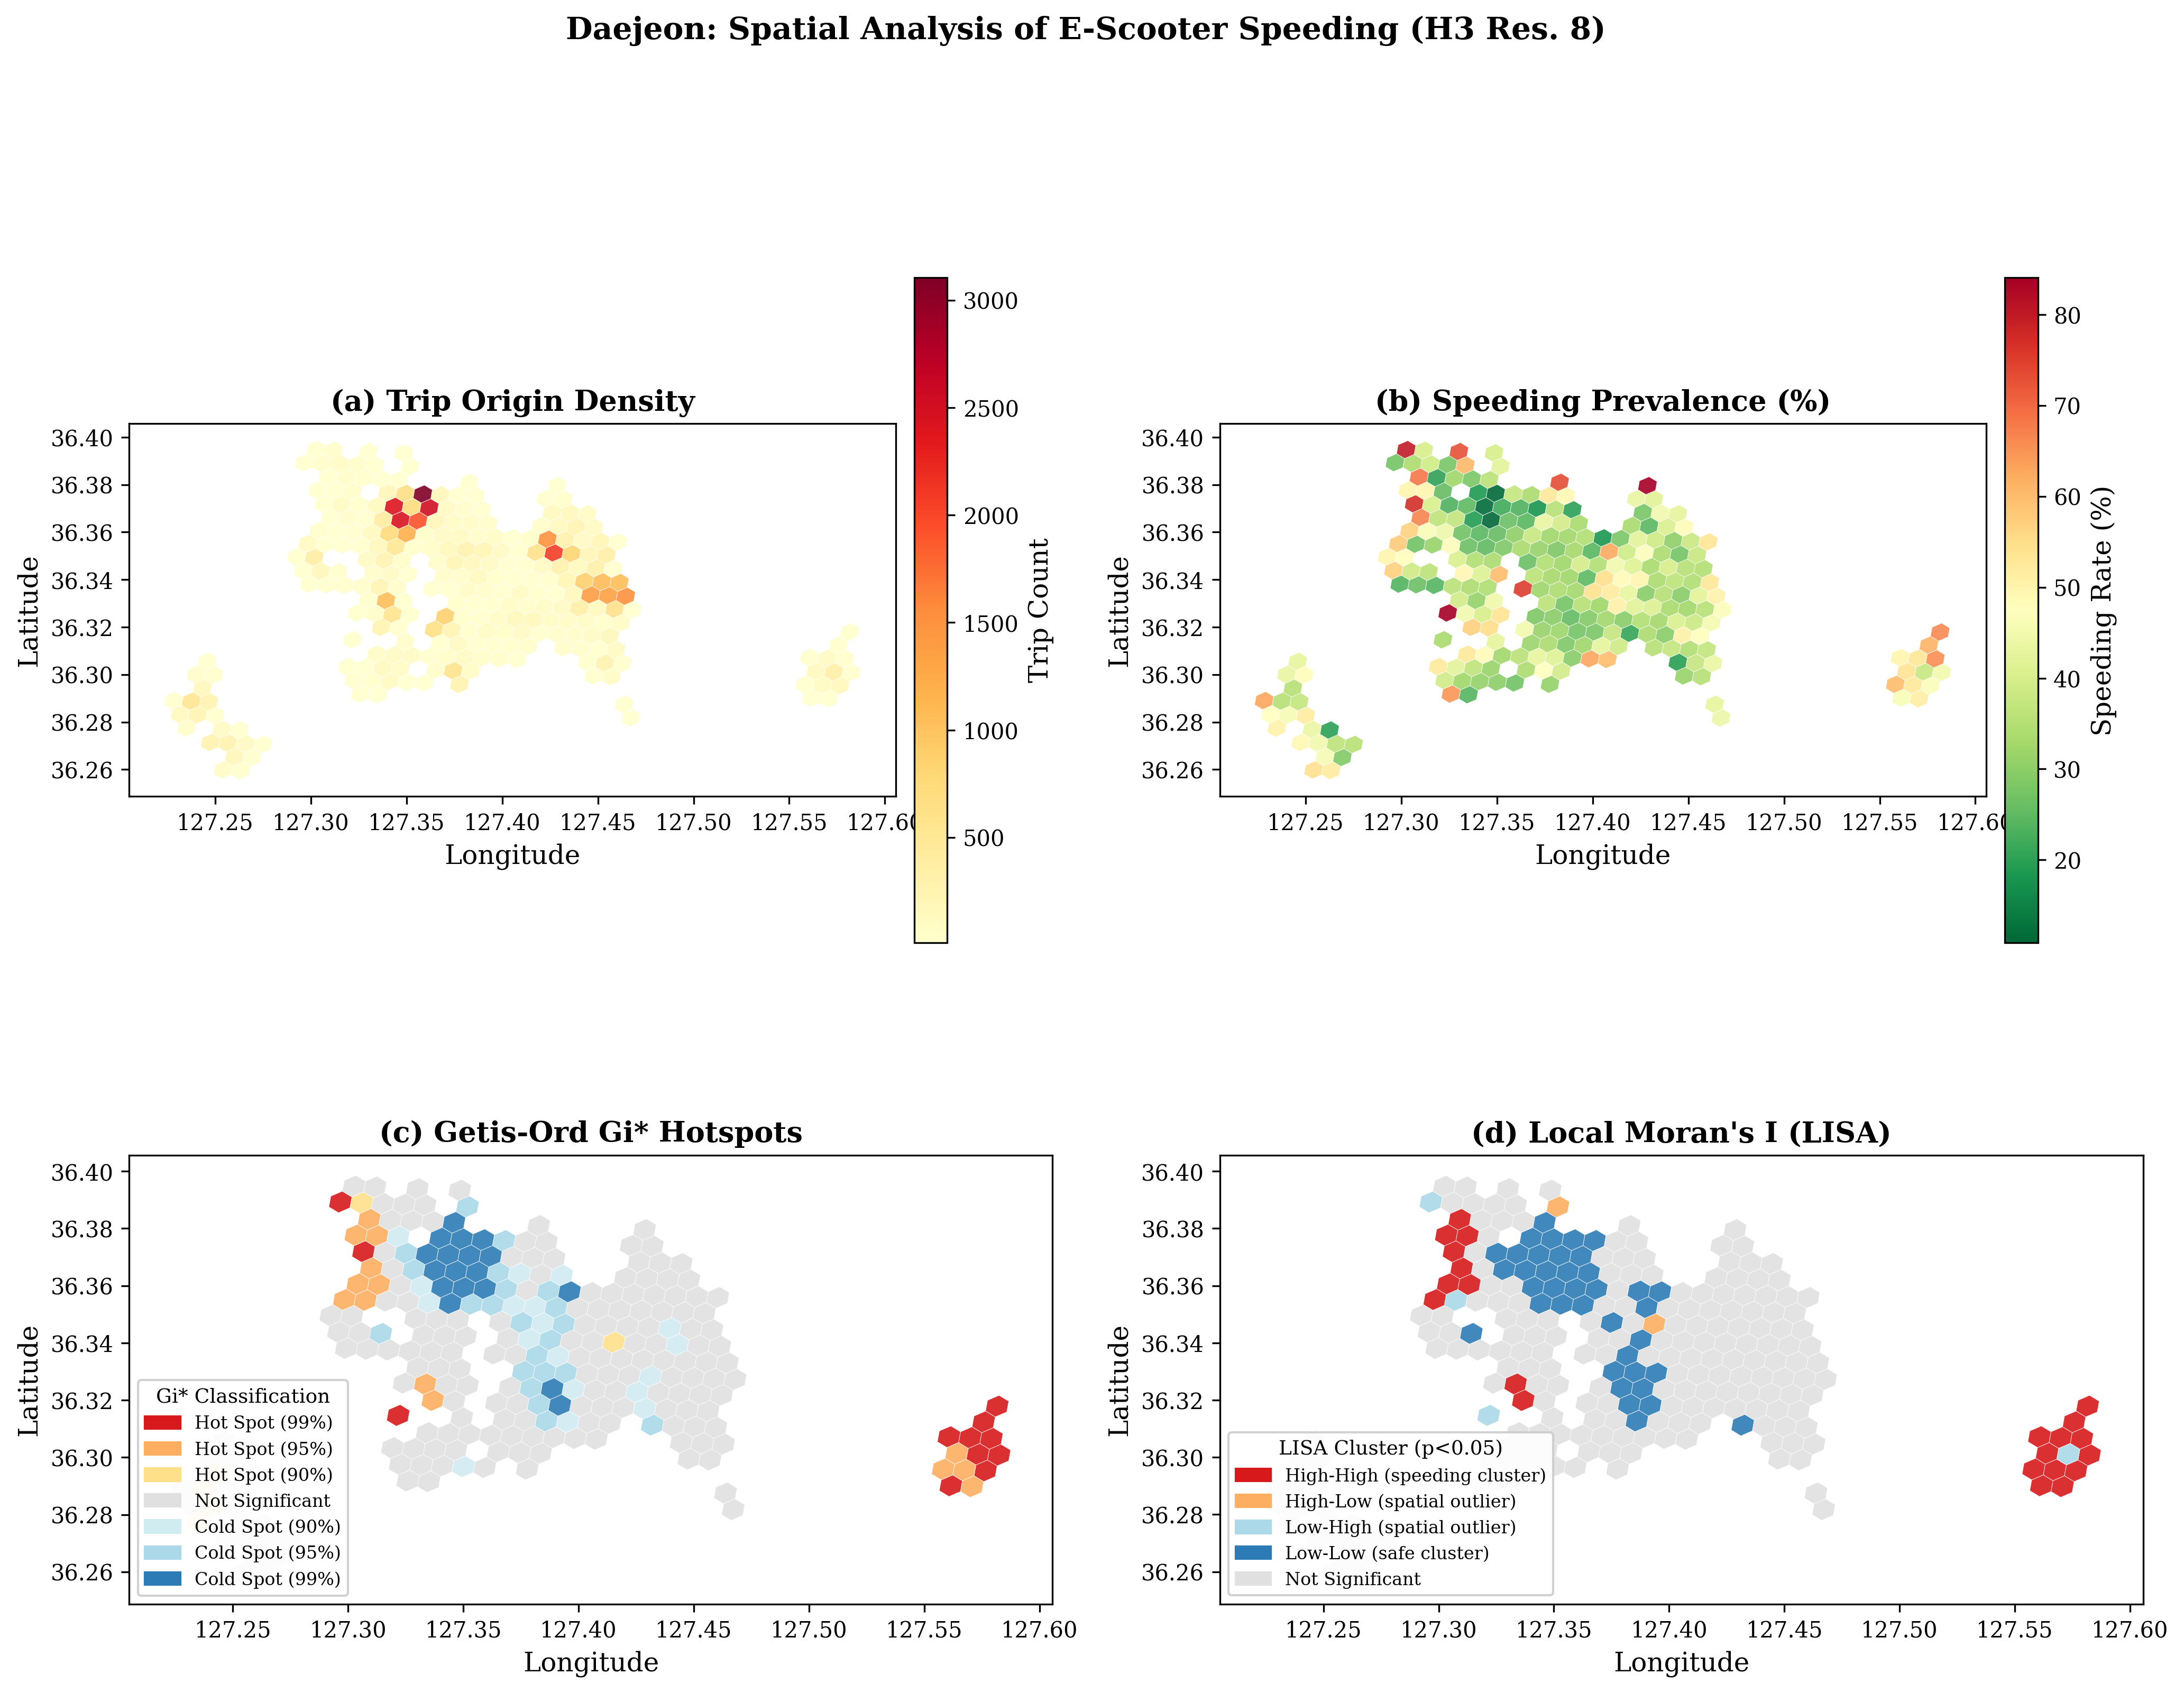
\includegraphics[width=\linewidth,height=0.52\textheight,keepaspectratio]{fig7_daejeon_hotspot.png}
  \vspace{-4pt}

  {\scriptsize Daejeon: Center-periphery pattern with hot spots in suburban arterials.}
\end{column}
\end{columns}

\vspace{3pt}
\centering
\scriptsize
\begin{tabular}{@{}l c c c@{}}
  \toprule
  \textbf{Seoul Hexes} & \textbf{Hot Spots} & \textbf{Not Sig.} & \textbf{Cold Spots} \\
  \midrule
  Mean speeding rate & 30.1\% & 22.4\% & 17.0\% \\
  Frac.\ major road & 0.210 & 0.207 & 0.207 \\
  Cycling infrastructure & 0.015 & 0.024 & 0.033 \\
  \bottomrule
\end{tabular}
\quad {\footnotesize Hot spots: \textbf{2$\times$ less} cycling infra than cold spots}
\end{frame}

% ═══════════════════════════════════════════════════════════════════════════
% SLIDE 11: SPATIAL ANALYSIS — Infrastructure & Clustering
% ═══════════════════════════════════════════════════════════════════════════
\begin{frame}{Spatial Analysis: Multi-City Clustering \& Infrastructure}
\begin{columns}[T]
\begin{column}{0.48\textwidth}
  \centering
  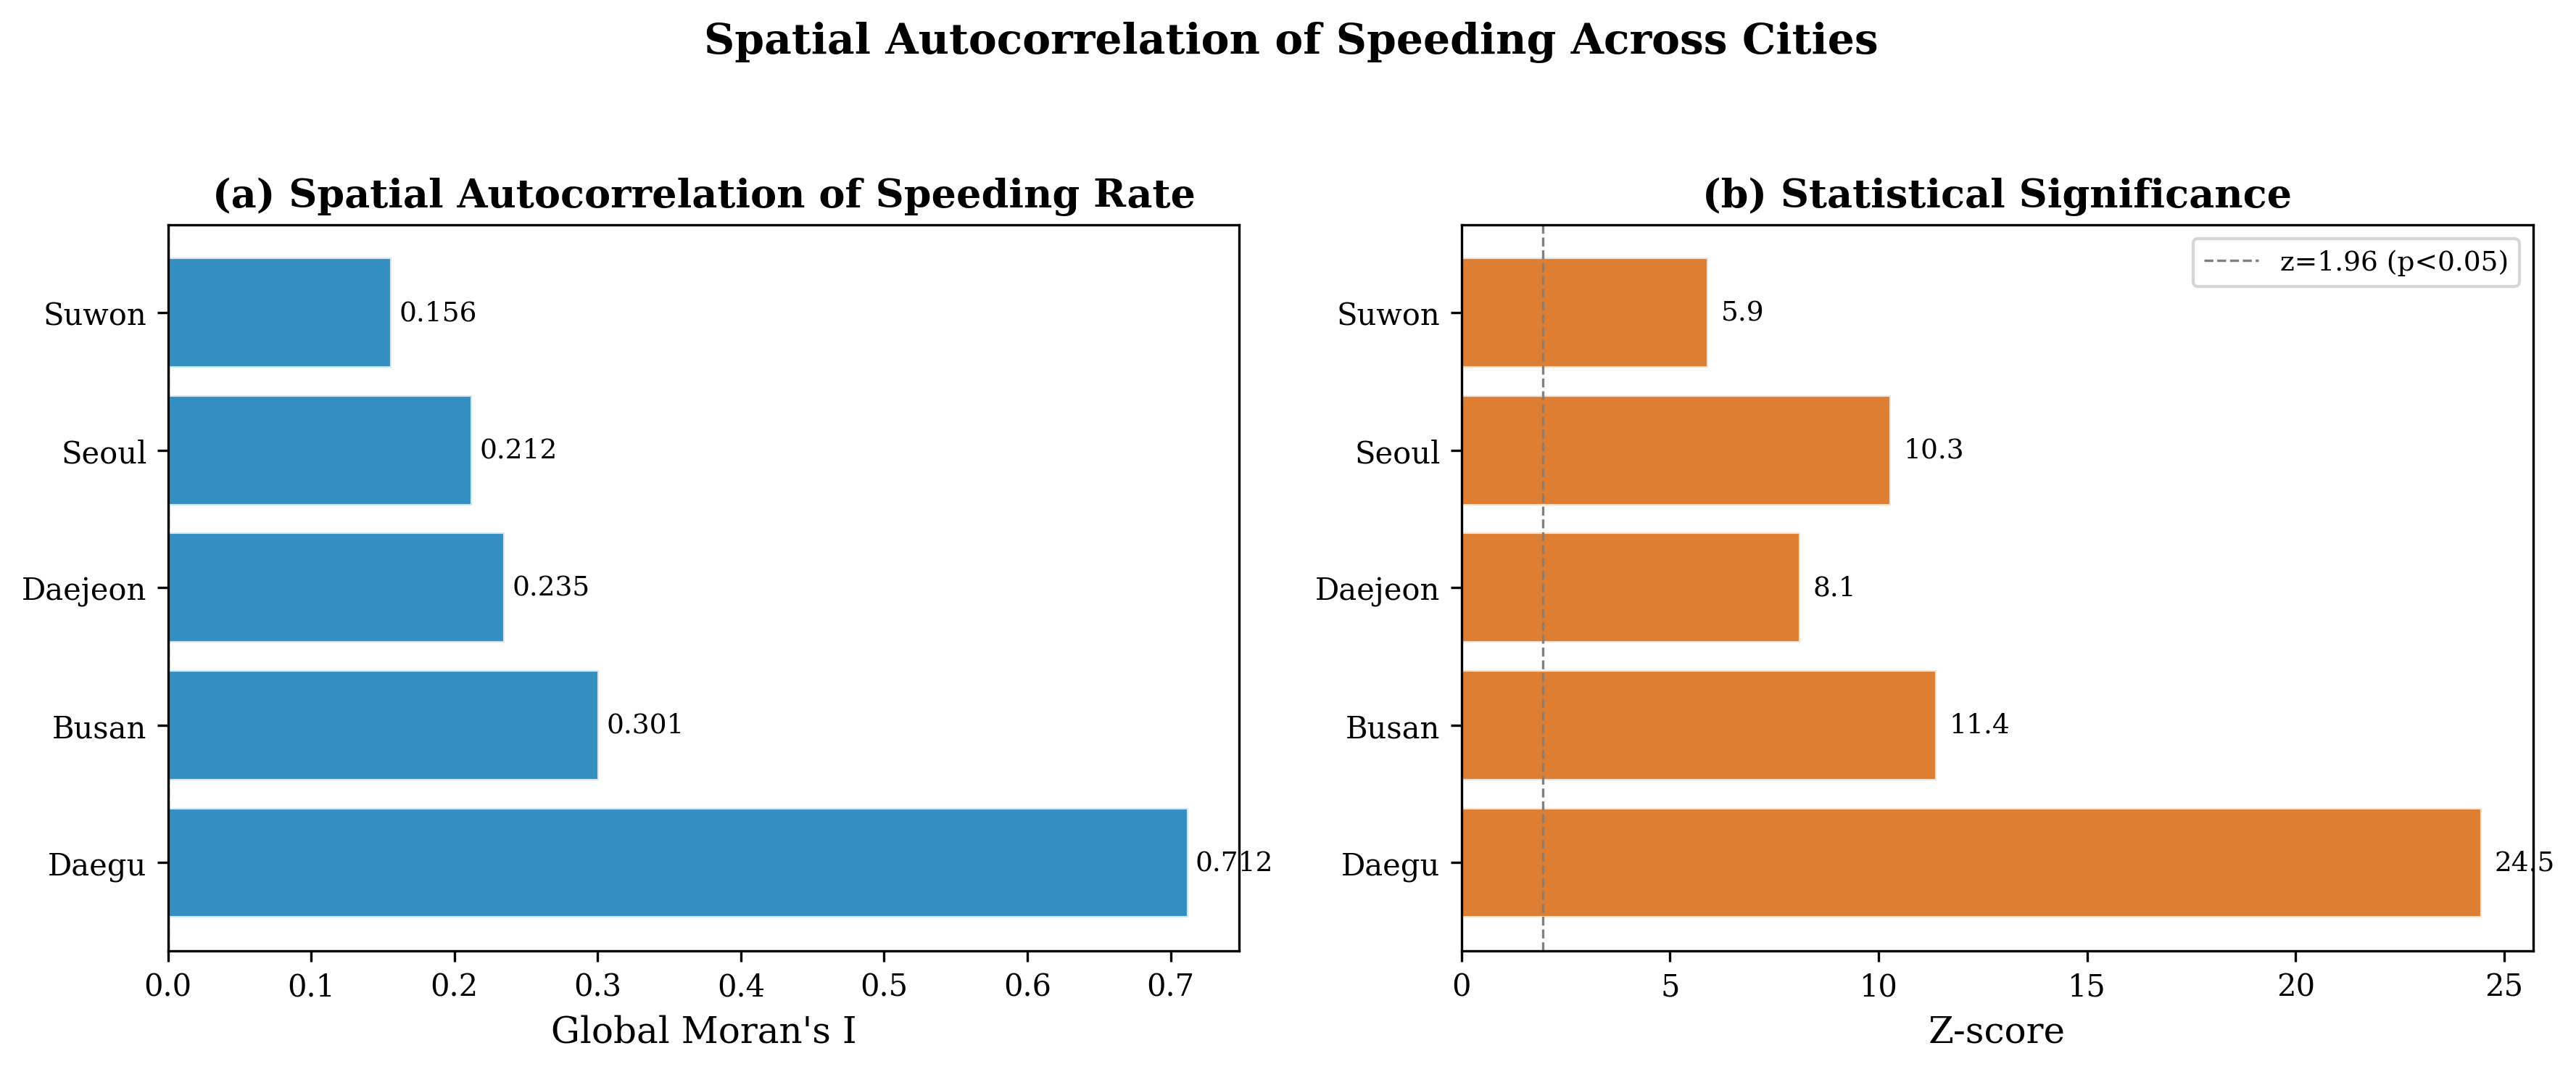
\includegraphics[width=\linewidth,height=0.33\textheight,keepaspectratio]{fig_morans_comparison.png}
  \vspace{-4pt}

  {\scriptsize Global Moran's $I$: all $p < 0.001$. Daegu: $I = 0.712$.}

  \vspace{1pt}
  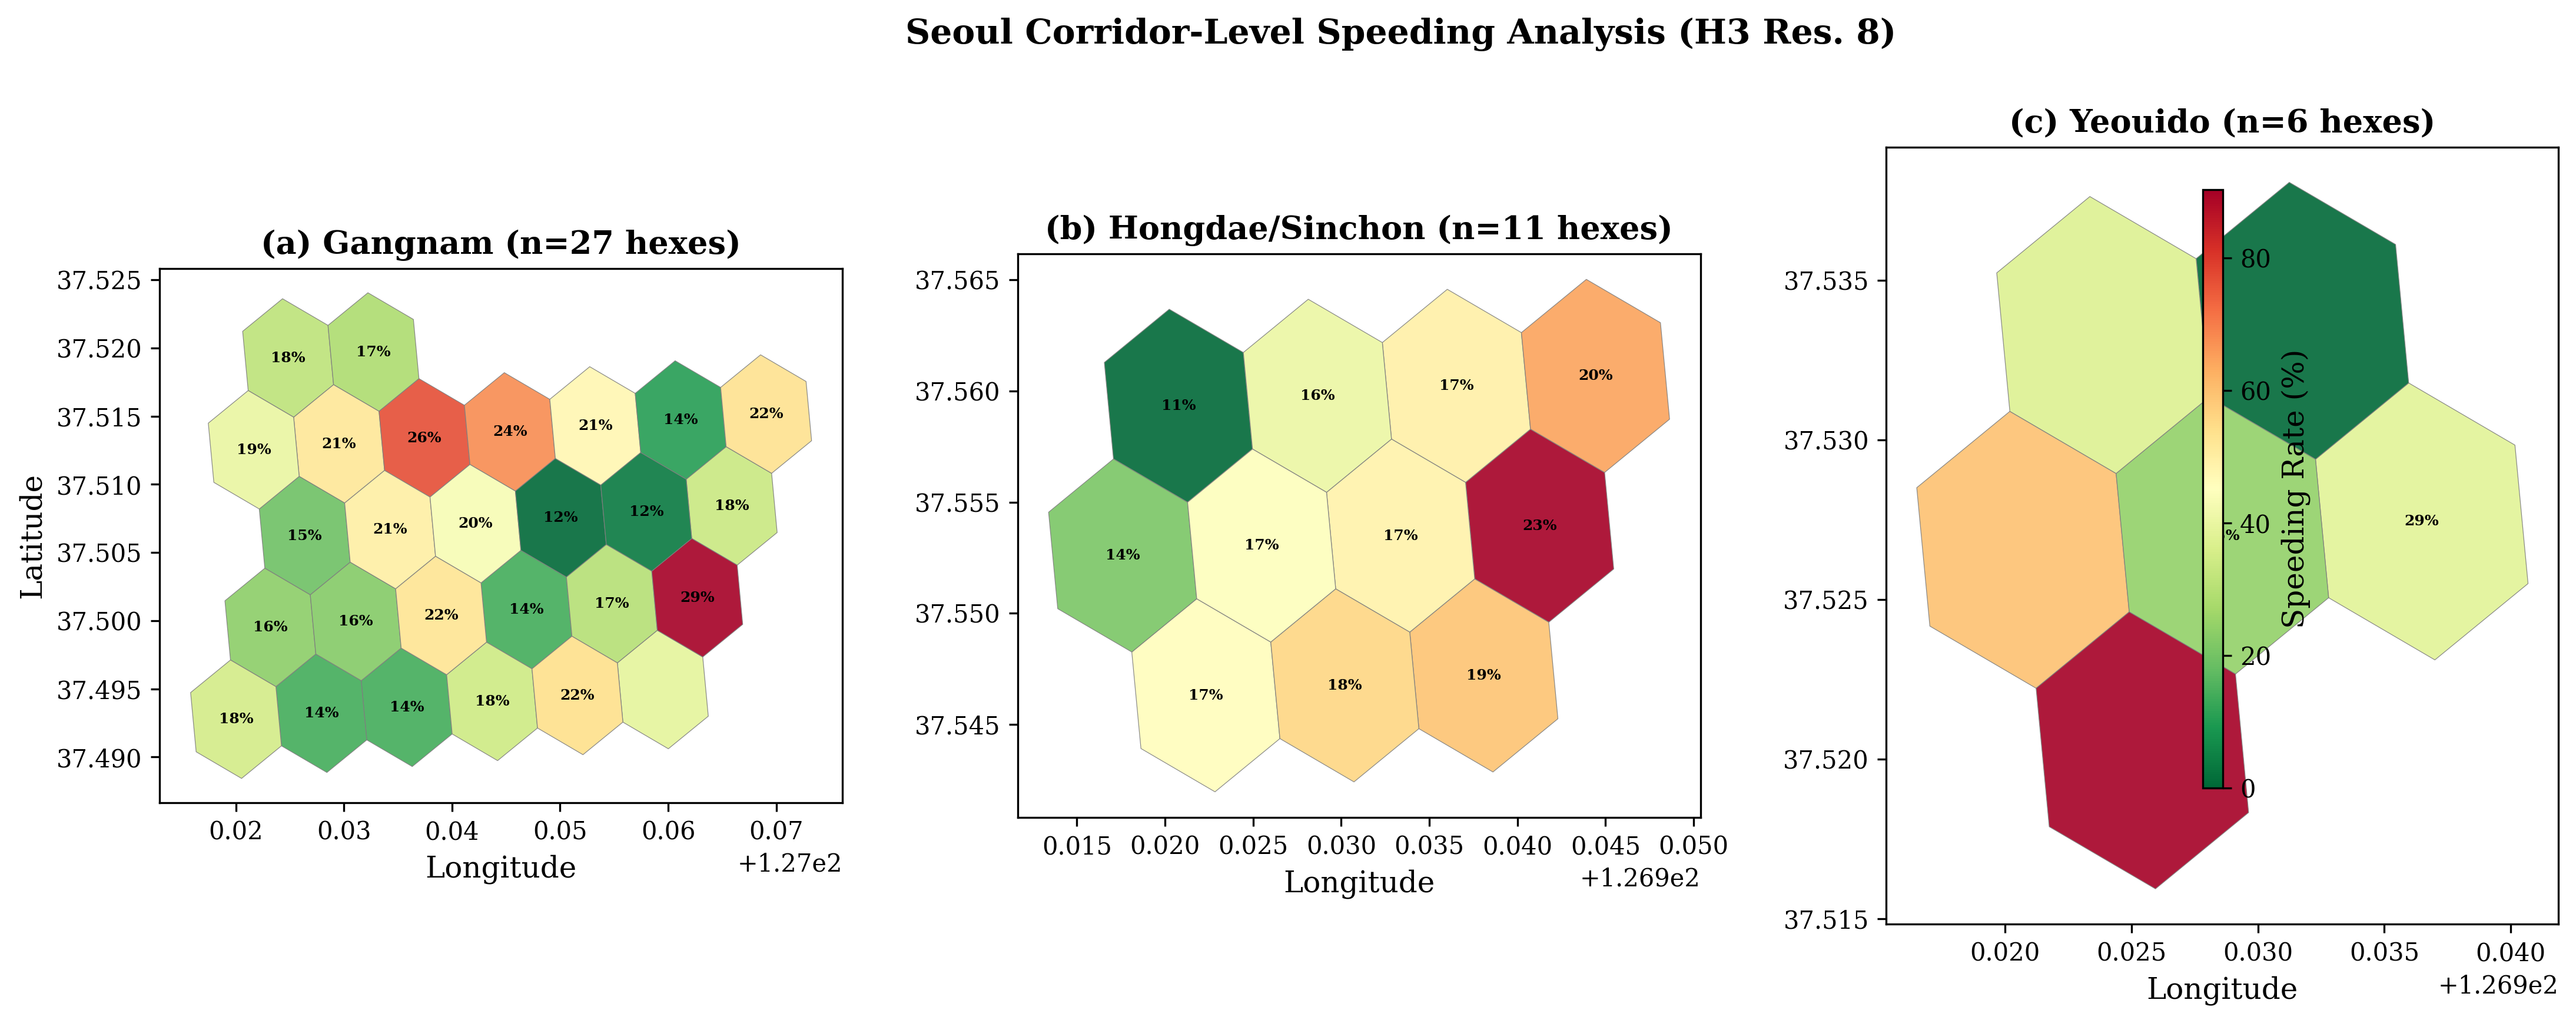
\includegraphics[width=\linewidth,height=0.22\textheight,keepaspectratio]{fig_corridor_speeding.png}
  \vspace{-4pt}

  {\scriptsize Seoul corridors: Gangnam, Hongdae, Yeouido. 10--80\% variation.}
\end{column}
\begin{column}{0.50\textwidth}
  \centering
  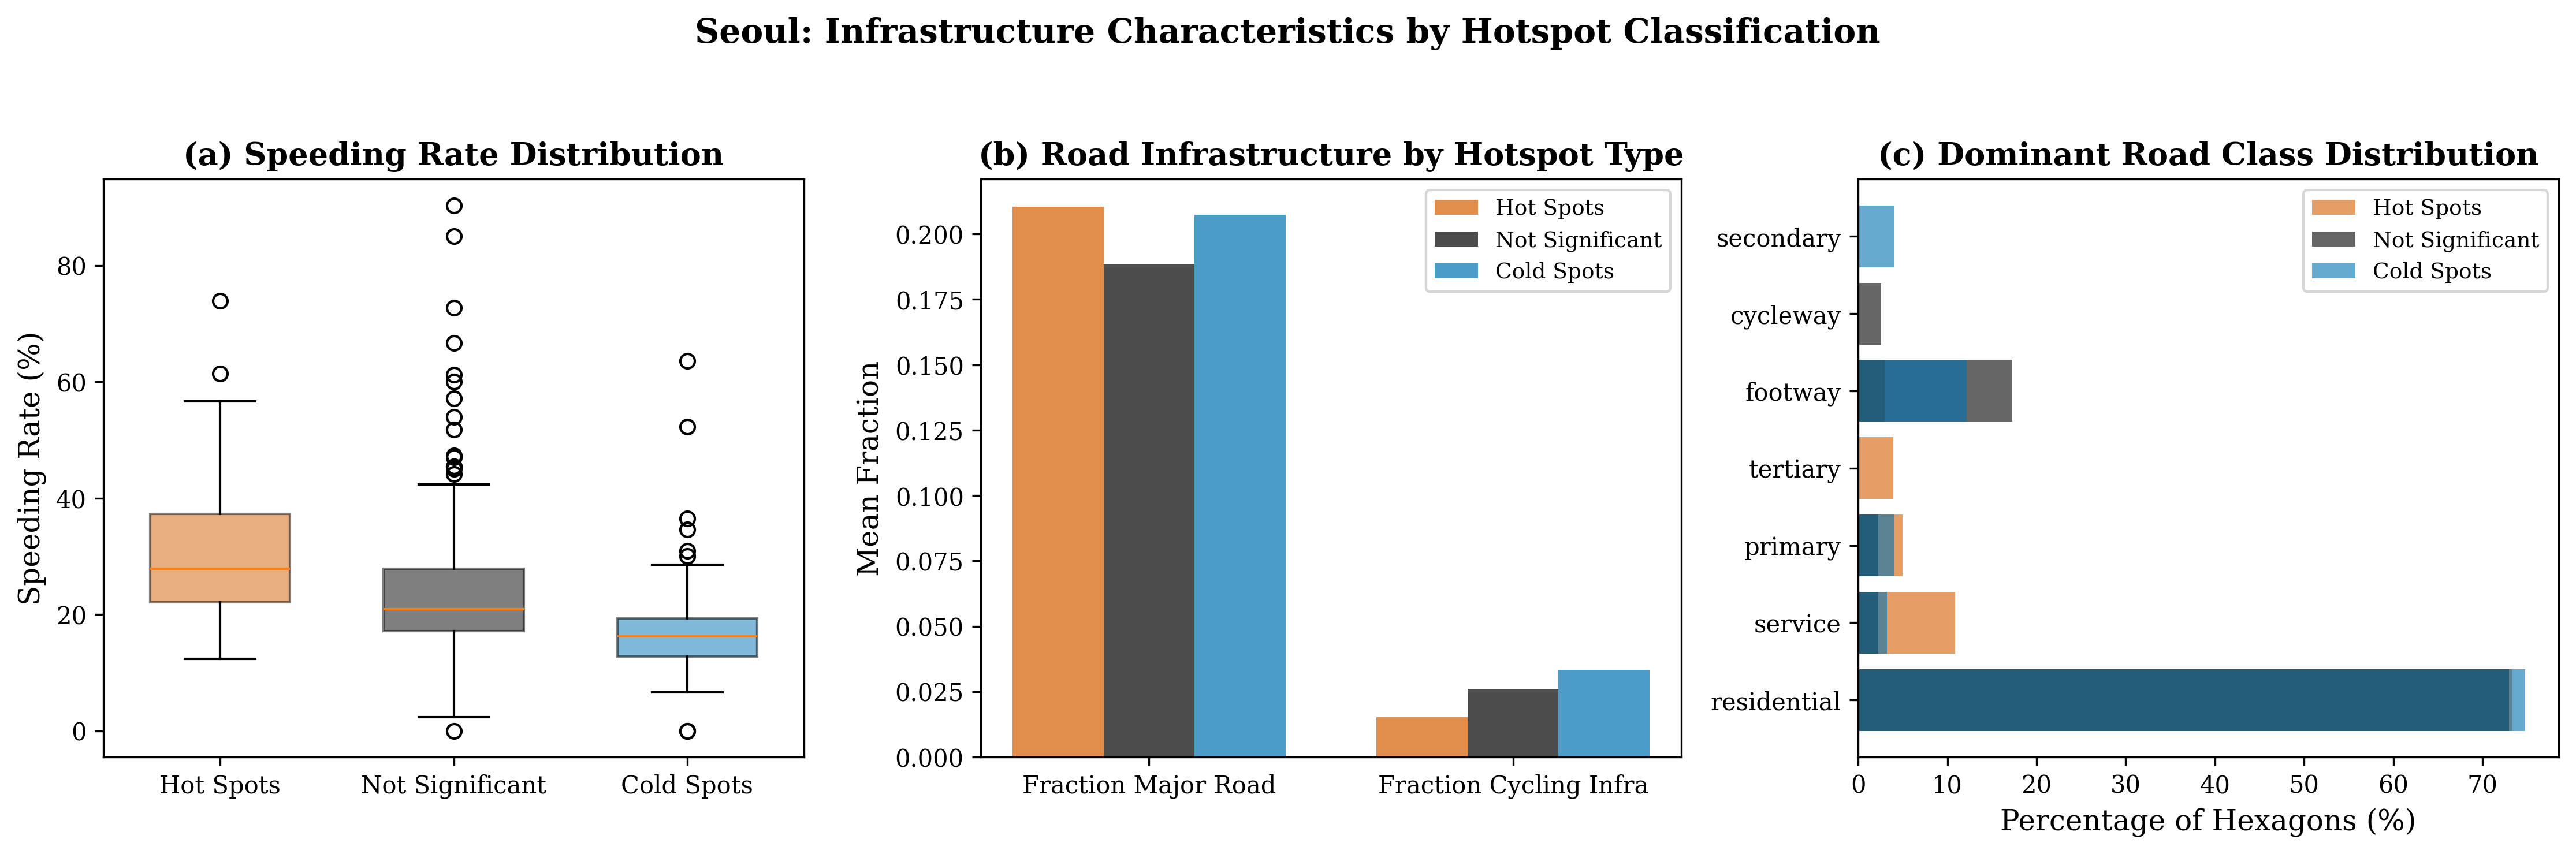
\includegraphics[width=\linewidth,height=0.35\textheight,keepaspectratio]{fig_hotspot_infrastructure.png}
  \vspace{-4pt}

  {\scriptsize Seoul: speeding, road infra, and road class by hotspot type.}

  \vspace{2pt}
  \scriptsize\textbf{Key Spatial Findings}
  \begin{itemize}\setlength\itemsep{0pt}\scriptsize
    \item Speeding is \textbf{spatially clustered}, not random
    \item Hot spots: less cycling infra, more major roads
    \item Provincial: Chungnam \textbf{45.8\%} vs.\ Ulsan \textbf{17.6\%}
    \item Adjacent hexes differ by 30+ pp
  \end{itemize}
\end{column}
\end{columns}
\end{frame}

% ═══════════════════════════════════════════════════════════════════════════
% SLIDE 12: MODEL DEVELOPMENT — Speeding Models
% ═══════════════════════════════════════════════════════════════════════════
\begin{frame}{Model Development: Speeding Propensity Models}
\begin{columns}[T]
\begin{column}{0.38\textwidth}
  \footnotesize
  \textbf{\textcolor{boxpurple}{Model Suite}}

  \vspace{2pt}
  \textbf{1.\ Logistic Regression} ($N{=}2.32$M)
  \begin{itemize}\setlength\itemsep{0pt}\scriptsize
    \item DV: any speeding event (binary)
    \item Mode, age, time, day, province
    \item Pseudo $R^2 = 0.354$
  \end{itemize}

  \vspace{2pt}
  \textbf{2.\ GEE Model} ($N{=}138{,}944$)
  \begin{itemize}\setlength\itemsep{0pt}\scriptsize
    \item Within-user correlation
    \item Exchangeable correlation, robust SE
  \end{itemize}

  \vspace{2pt}
  \textbf{3.\ Mixed-Effects LM} ($N{=}100{,}000$)
  \begin{itemize}\setlength\itemsep{0pt}\scriptsize
    \item DV: mean trip speed (continuous)
    \item Random intercepts for user
    \item ICC $= 0.271$ (27\% between-user)
  \end{itemize}

  \vspace{2pt}
  \textbf{4.\ Two-Part Hurdle}
  \begin{itemize}\setlength\itemsep{0pt}\scriptsize
    \item Part 1: Logistic (any speeding)
    \item Part 2: Beta (rate $|$ speeding $>0$)
    \item Handles 70.4\% zero inflation
  \end{itemize}
\end{column}
\begin{column}{0.60\textwidth}
  \centering
  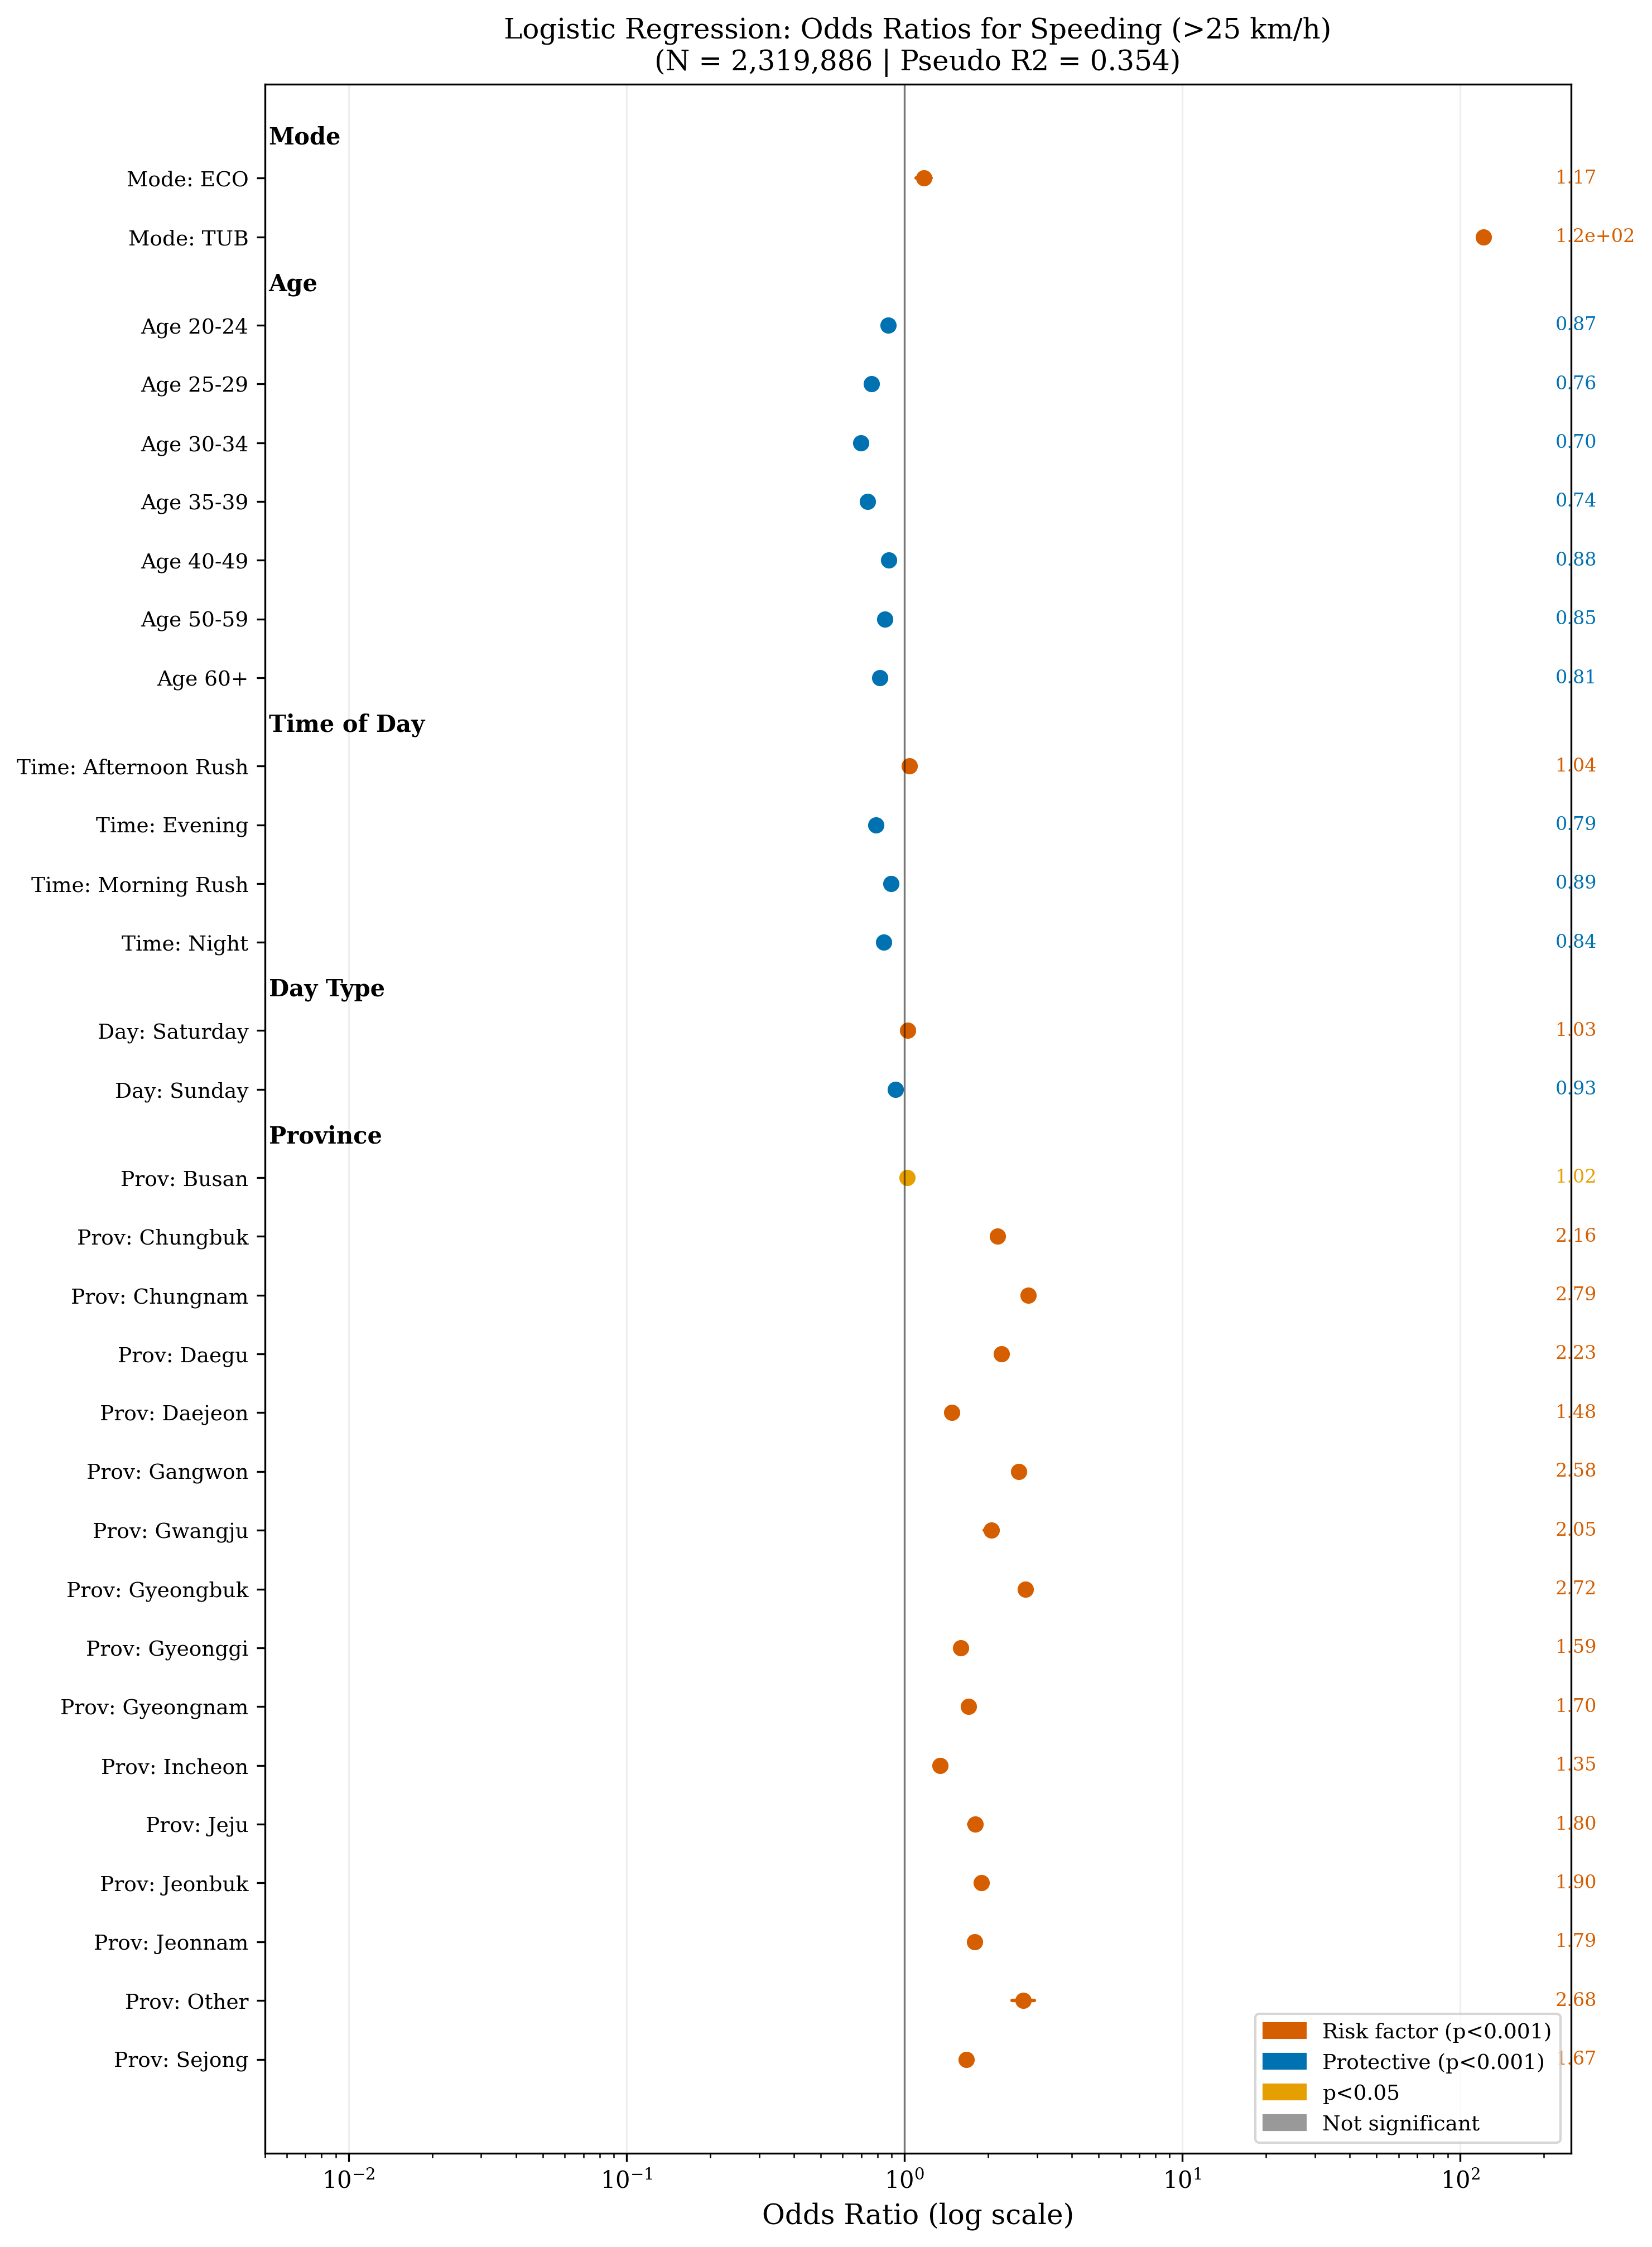
\includegraphics[width=0.88\linewidth,height=0.75\textheight,keepaspectratio]{fig9_logistic_OR.png}
  \vspace{-4pt}

  {\scriptsize Logistic OR (log scale). TUB: OR $= 121$. Age 30--34: OR $= 0.70$ (lowest risk). Chungnam: OR $= 2.79$ (highest province).}
\end{column}
\end{columns}
\end{frame}

% ═══════════════════════════════════════════════════════════════════════════
% SLIDE 13: MODEL DEVELOPMENT — Mixed Effects & GMM
% ═══════════════════════════════════════════════════════════════════════════
\begin{frame}{Model Development: Mean Speed Model \& Rider Typology}
\begin{columns}[T]
\begin{column}{0.47\textwidth}
  \centering
  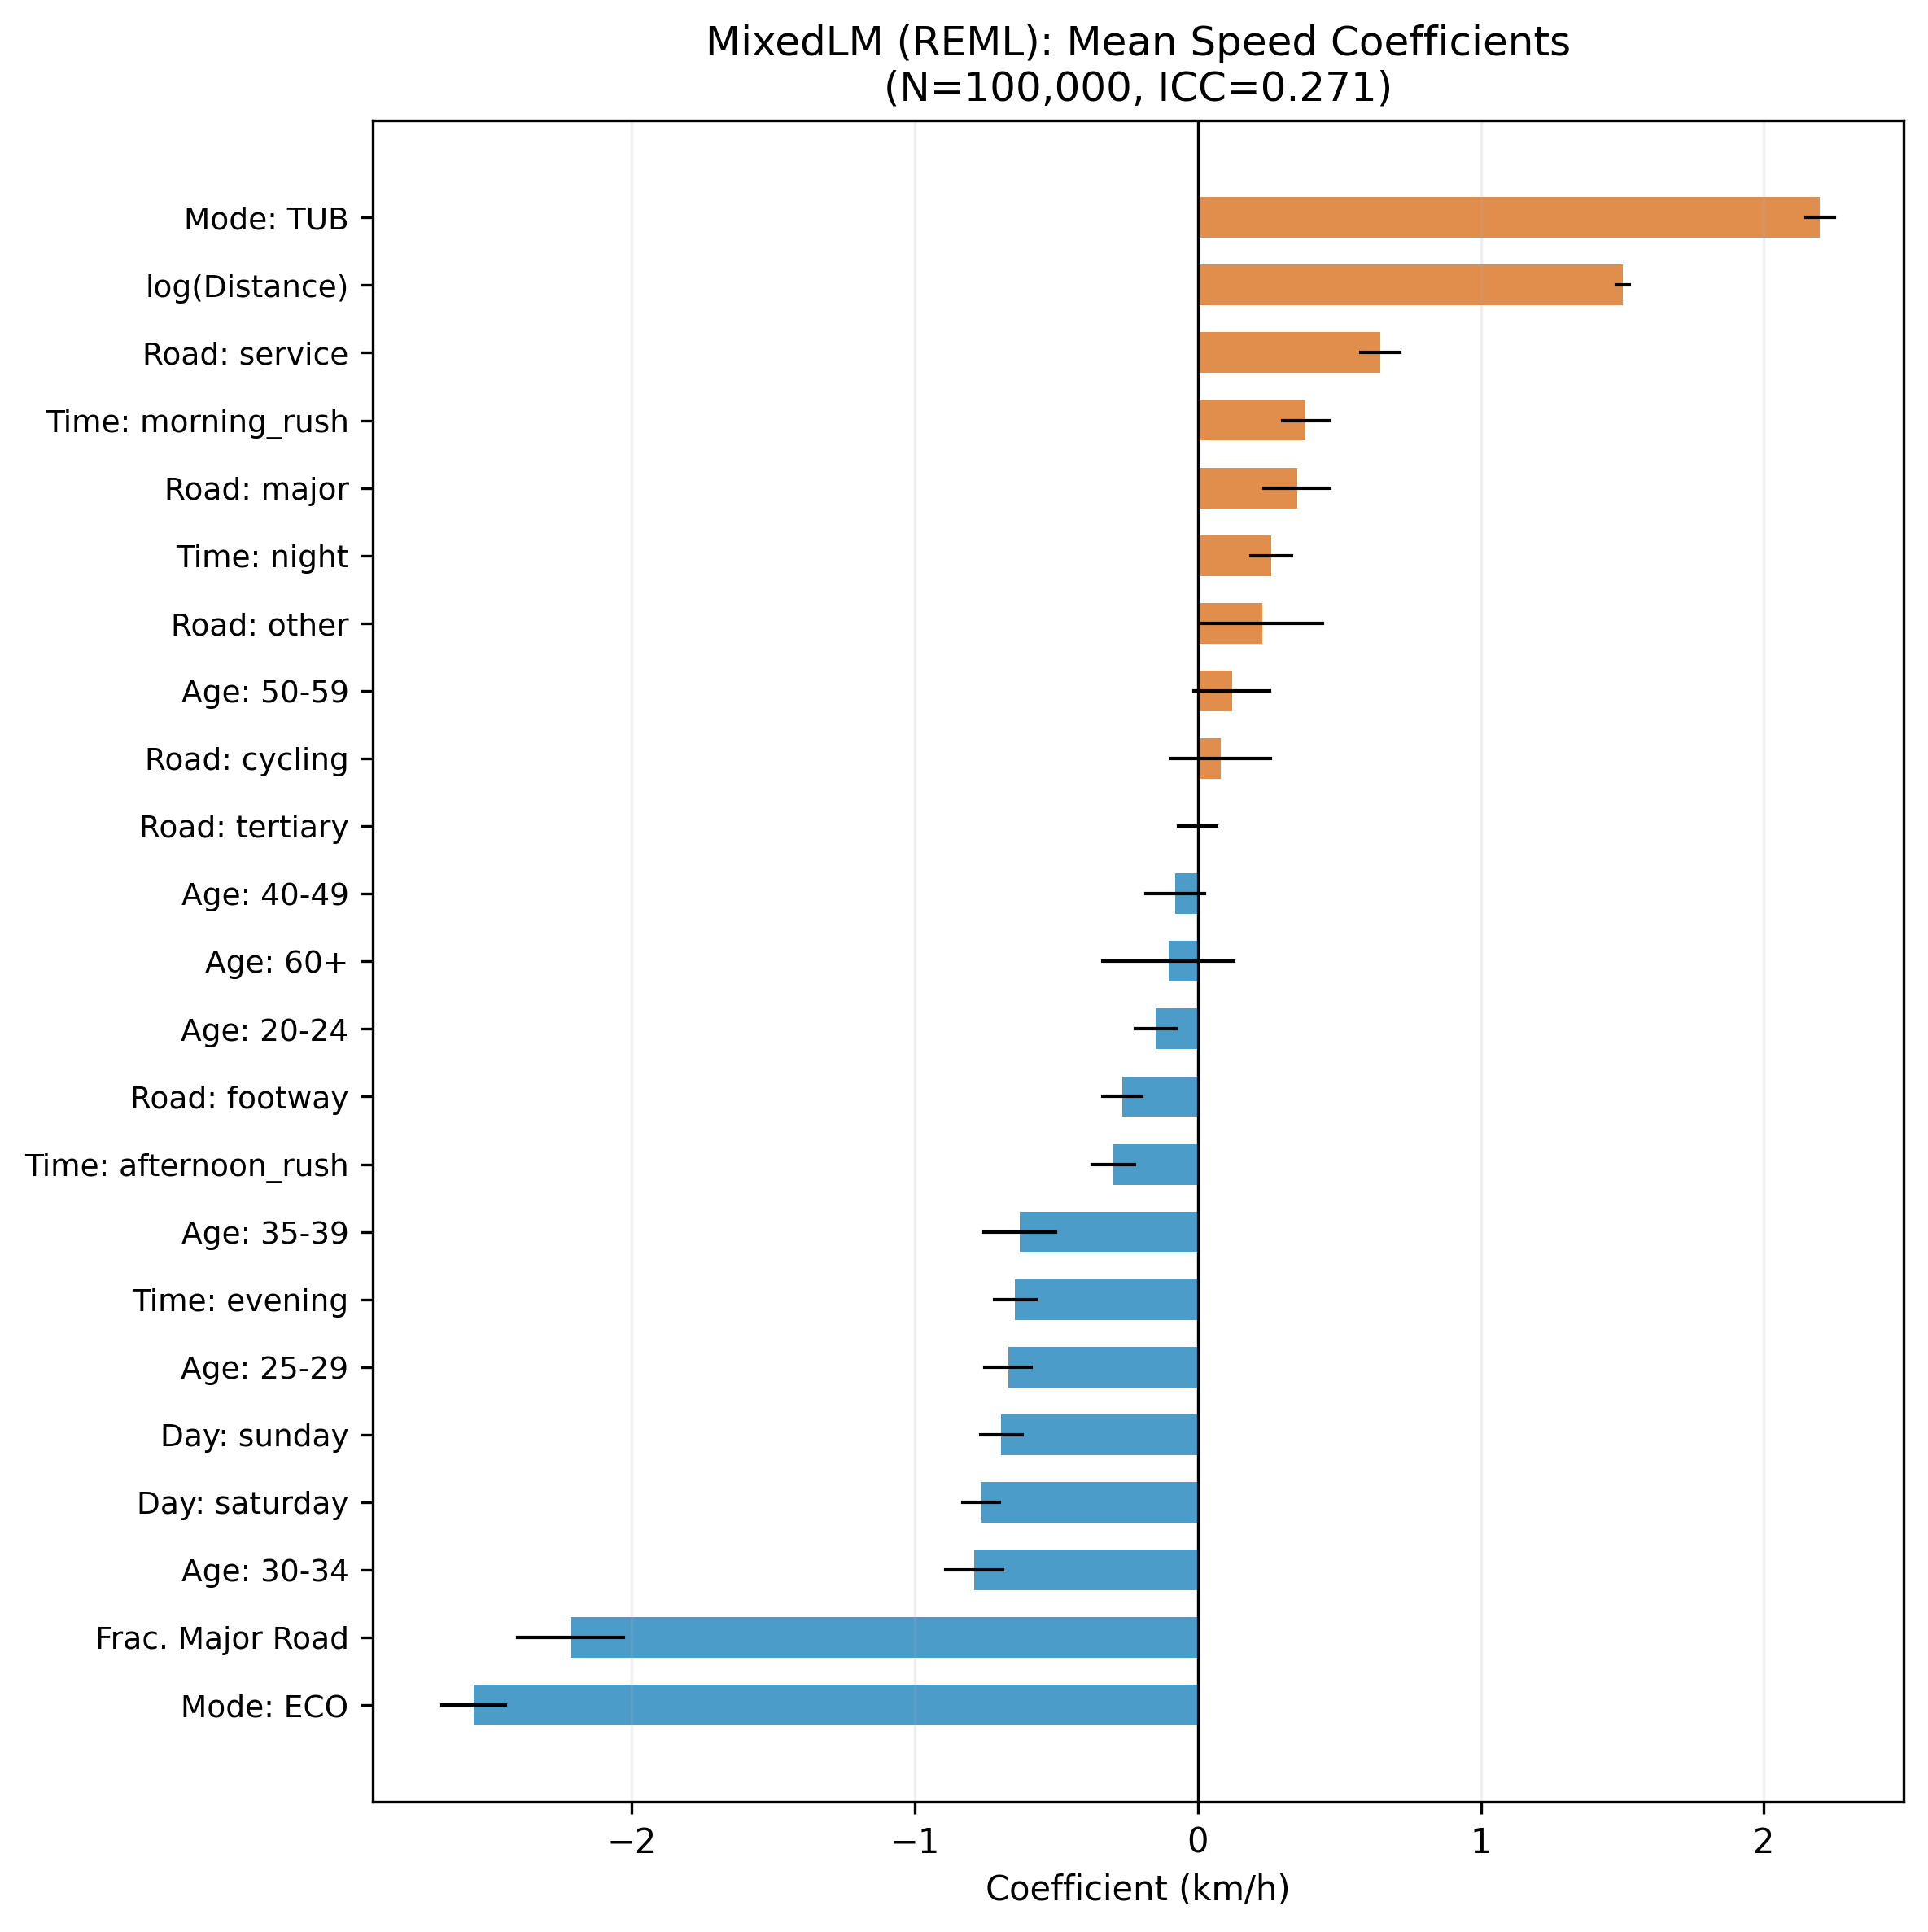
\includegraphics[width=\linewidth,height=0.72\textheight,keepaspectratio]{fig_mixed_effects_coefficients.png}
  \vspace{-4pt}

  {\scriptsize Mixed LM (REML) coefficients in km/h. TUB: $+2.2$; ECO: $-2.6$ vs.\ STD. Frac.\ major road: $-2.2$ (congestion). ICC $= 0.271$.}
\end{column}
\begin{column}{0.51\textwidth}
  \centering
  \includegraphics[width=0.82\linewidth]{gmm_profiles_k4.png}
  \vspace{-4pt}

  {\scriptsize GMM ($K{=}4$) profiles on 11 normalized speed indicators per user.}

  \vspace{2pt}
  \scriptsize
  \begin{tabular}{@{}l c l@{}}
    \toprule
    \textbf{Class} & \textbf{\%} & \textbf{Profile} \\
    \midrule
    Safe Rider & 40\% & Low speed, low variability \\
    Moderate Risk & 26\% & Mid speed, some speeding \\
    Habitual Speeder & 26\% & High max, high propensity \\
    Stop-and-Go & 8\% & High accel, high zero-frac \\
    \bottomrule
  \end{tabular}
\end{column}
\end{columns}
\end{frame}

% ═══════════════════════════════════════════════════════════════════════════
% SLIDE 14: RESULTS — Speed Governor Effect
% ═══════════════════════════════════════════════════════════════════════════
\begin{frame}{Results: Speed Governor Effect (TUB vs.\ ECO)}
\begin{columns}[T]
\begin{column}{0.55\textwidth}
  \centering
  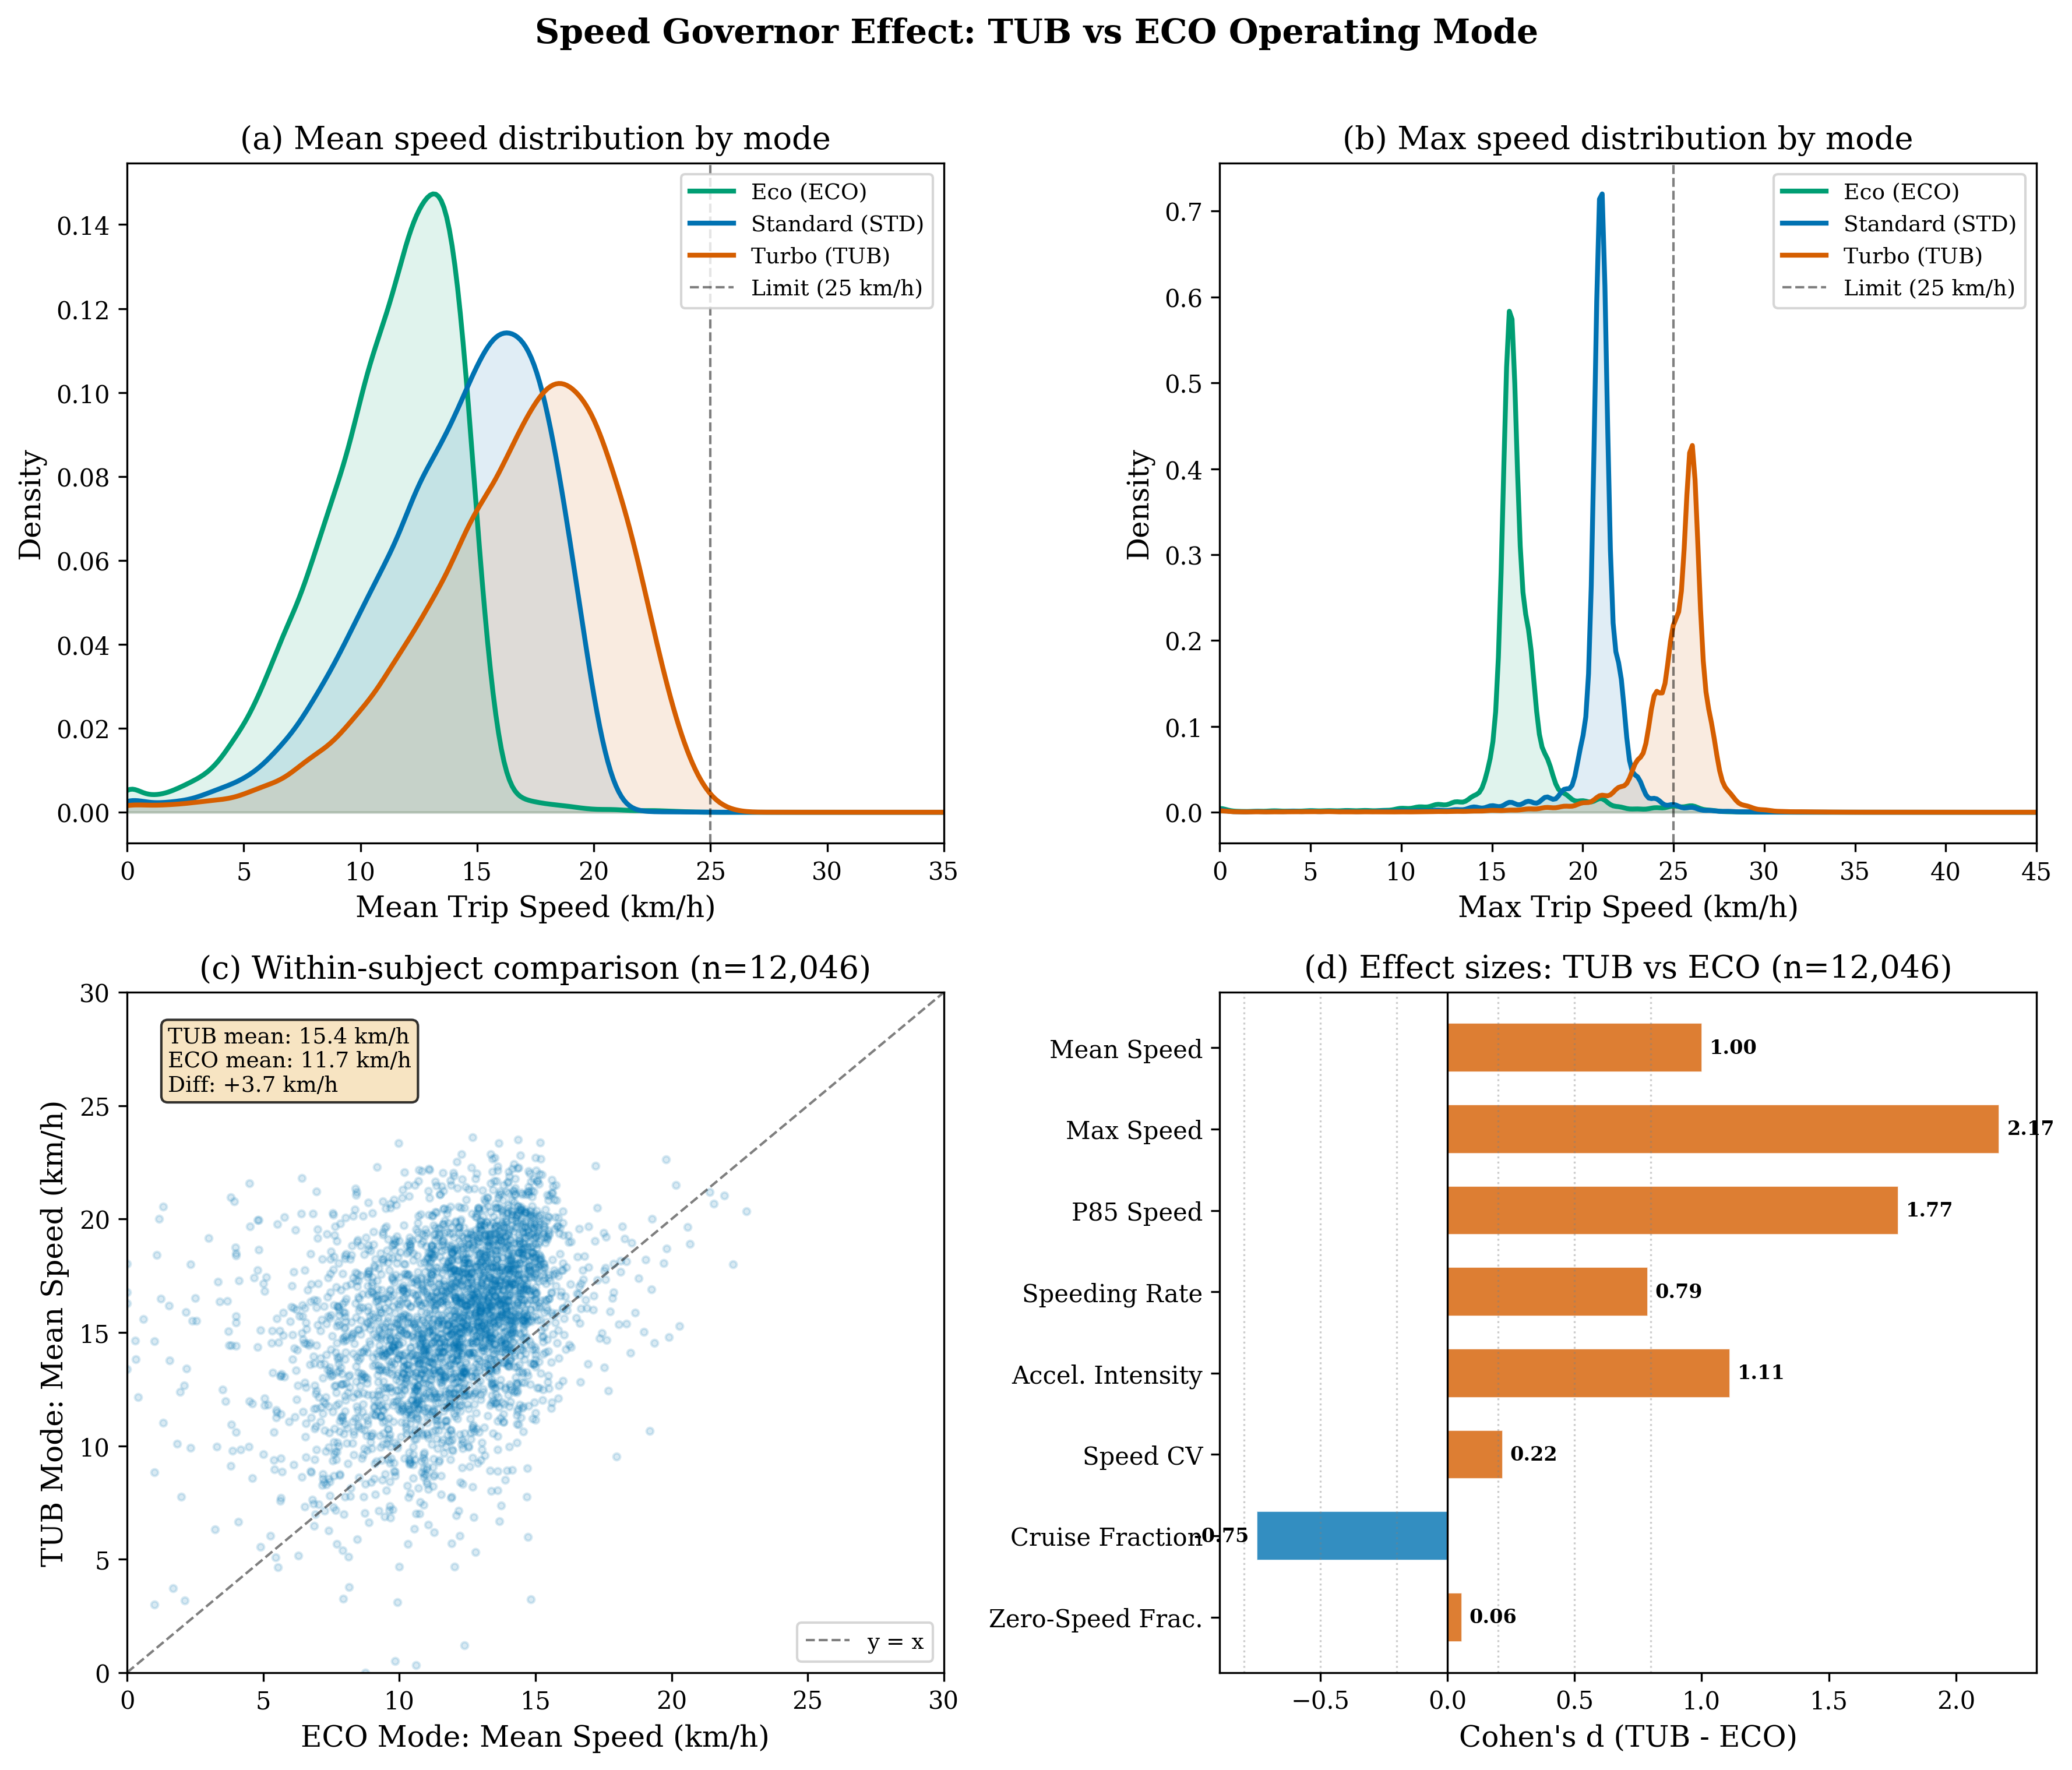
\includegraphics[width=\linewidth,height=0.62\textheight,keepaspectratio]{fig12_tub_vs_eco.png}
  \vspace{-4pt}

  {\scriptsize (a) Mean speed by mode. (b) Max speed: ECO $<$18 km/h. (c) Paired ($n{=}12{,}046$): diff $= +3.7$ km/h. (d) Cohen's $d$.}
\end{column}
\begin{column}{0.43\textwidth}
  \centering
  \includegraphics[width=\linewidth,height=0.26\textheight,keepaspectratio]{mode_paired_analysis.png}
  \vspace{-4pt}

  {\scriptsize Same 12,046 users in both modes. Points above diagonal $=$ higher TUB speed.}

  \vspace{3pt}
  \footnotesize\textbf{Key Results}
  \begin{itemize}\setlength\itemsep{0pt}\scriptsize
    \item ECO governor: speeding \textbf{54\% $\to$ 1.1\%}
    \item 34\% mean speed reduction
    \item Cohen's $d$: 1.00 (mean), 2.17 (max), 1.77 (P85)
    \item All within-subject $p < 0.001$
    \item \textbf{Most effective single intervention}
  \end{itemize}
\end{column}
\end{columns}
\end{frame}

% ═══════════════════════════════════════════════════════════════════════════
% SLIDE 15: RESULTS — GEE & Demographics
% ═══════════════════════════════════════════════════════════════════════════
\begin{frame}{Results: GEE Model \& Demographic Effects}
\begin{columns}[T]
\begin{column}{0.45\textwidth}
  \centering
  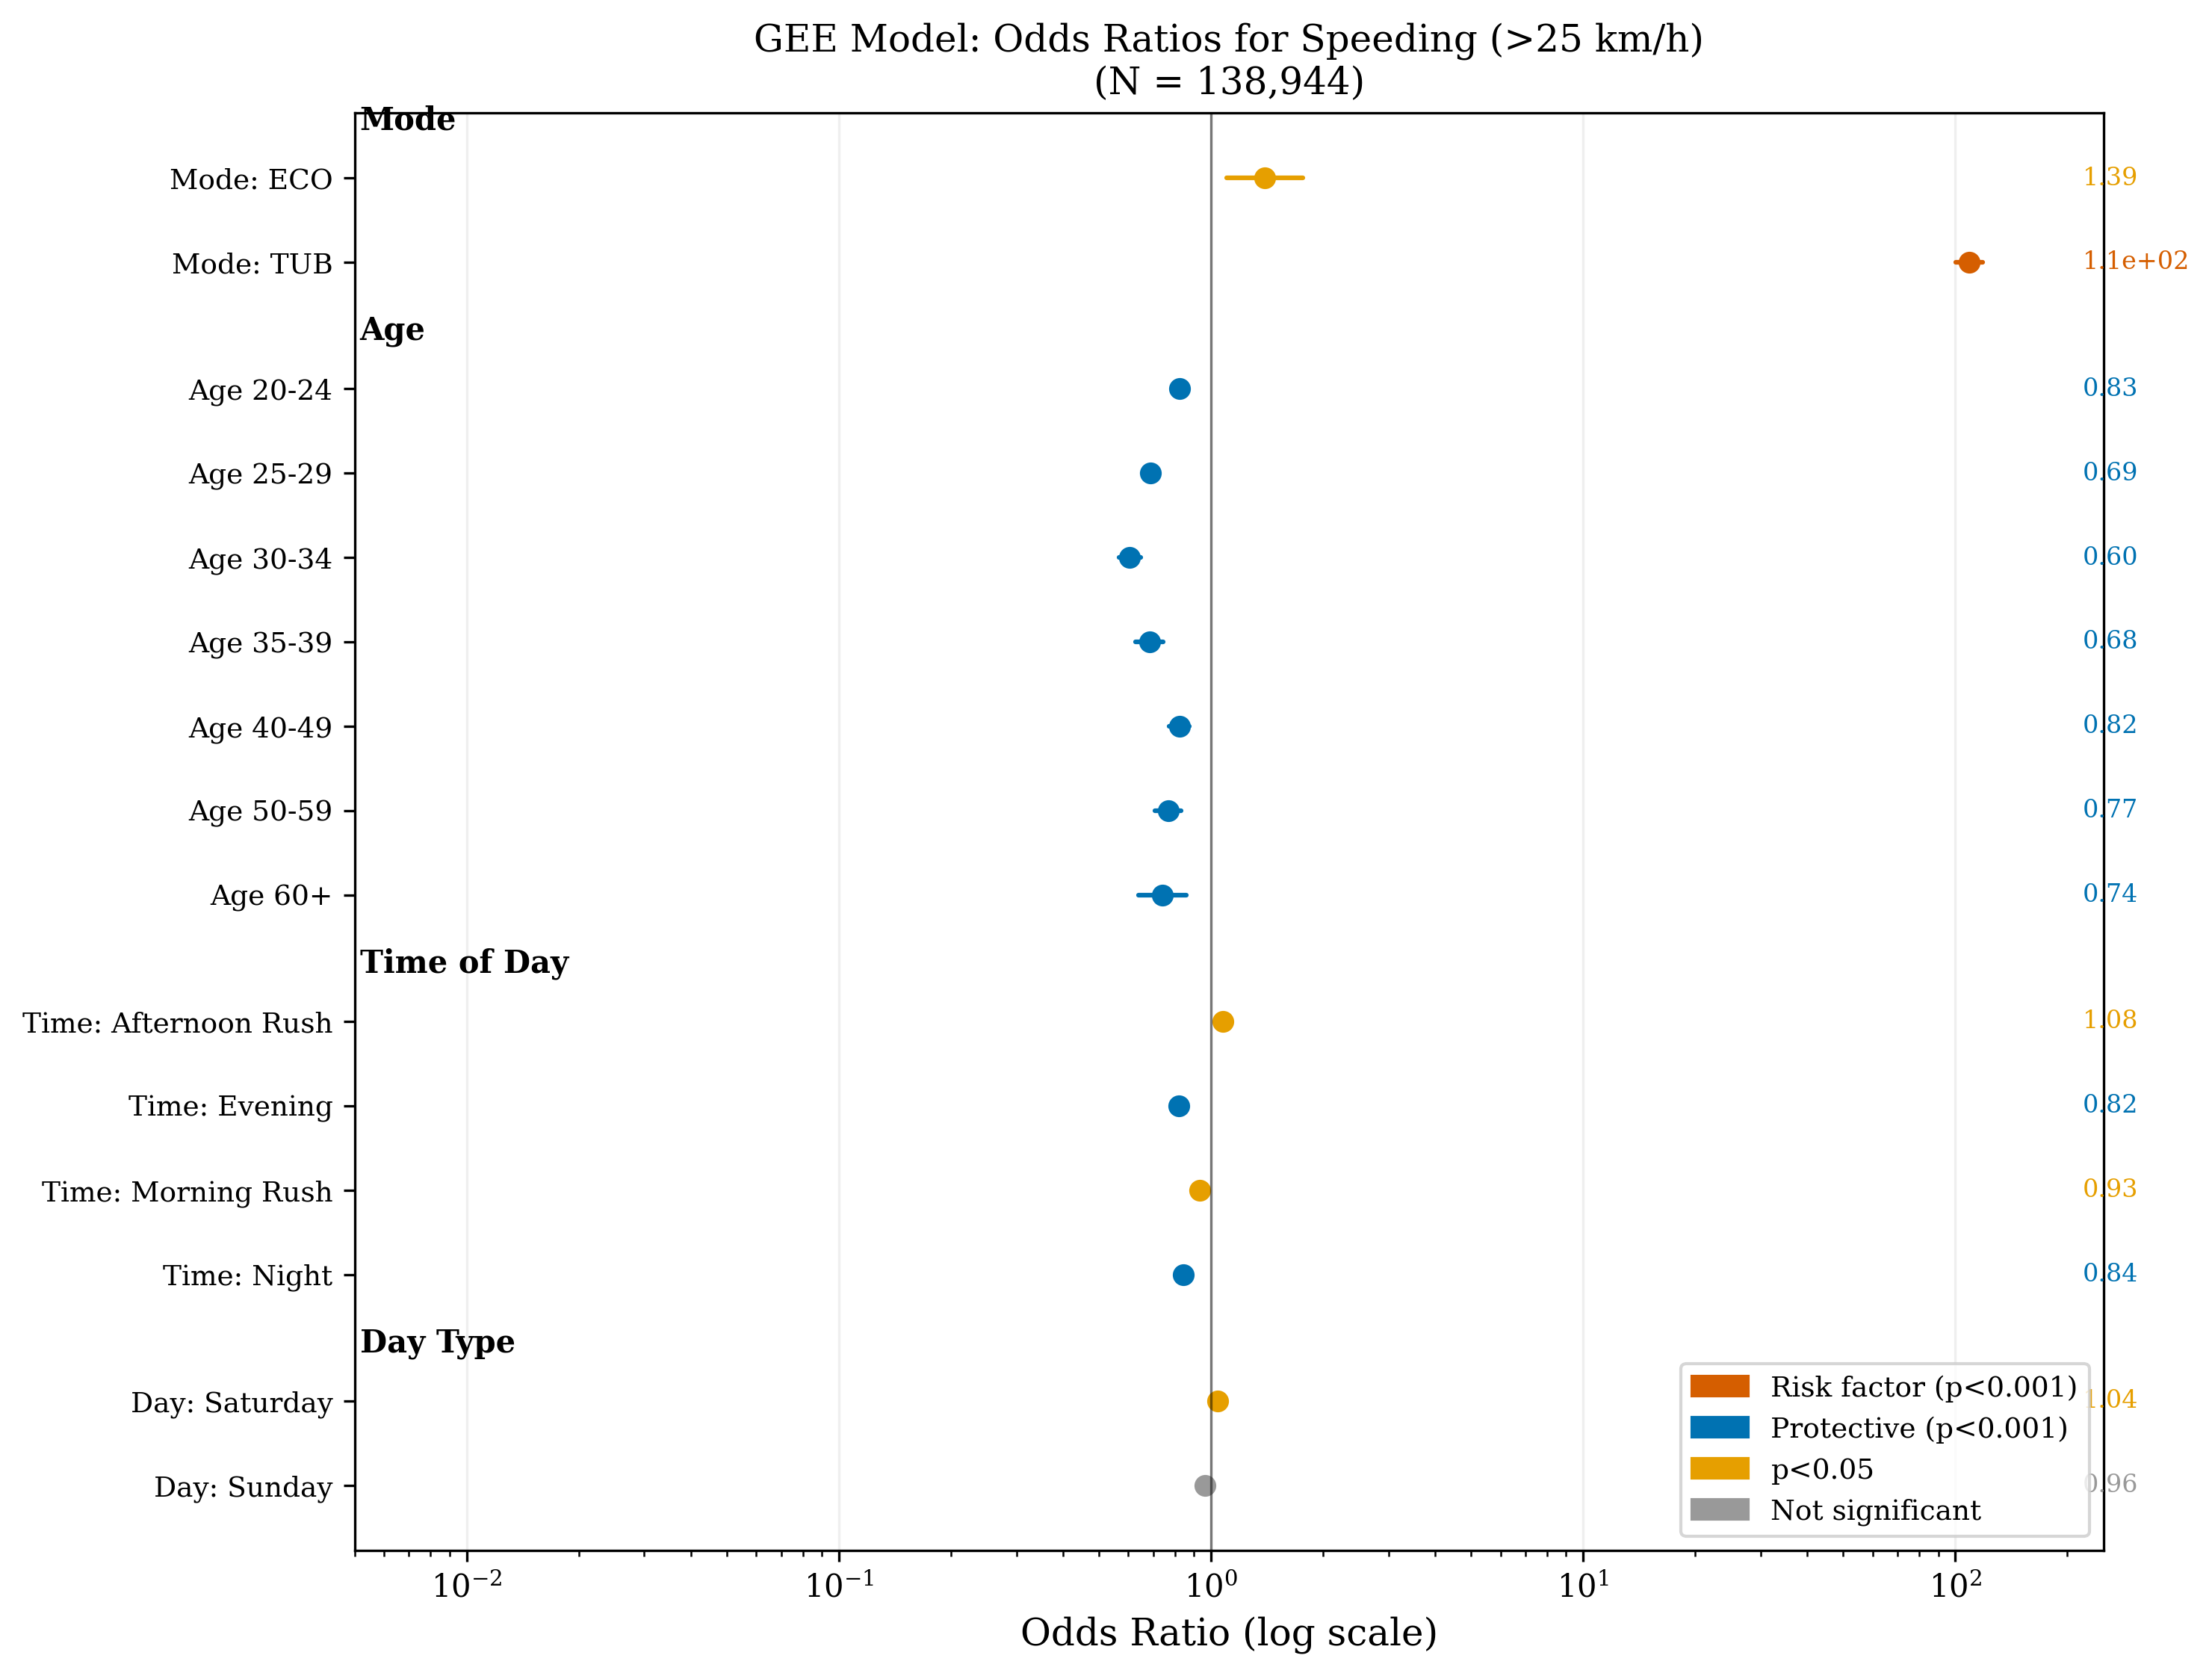
\includegraphics[width=\linewidth,height=0.72\textheight,keepaspectratio]{fig10_gee_OR.png}
  \vspace{-4pt}

  {\scriptsize GEE ($N{=}138{,}944$) with within-user correlation. TUB OR $= 110$. Age 30--34: OR $= 0.60$.}
\end{column}
\begin{column}{0.53\textwidth}
  \scriptsize
  \textbf{\textcolor{boxred}{Age Effects}} (vs.\ under-20 reference)
  \begin{itemize}\setlength\itemsep{0pt}
    \item Ages 20--24: OR $= 0.83$ (protective)
    \item \textbf{Ages 30--34: OR $= 0.60$} (safest group)
    \item Ages 60+: OR $= 0.74$
    \item Under-20 highest risk; 30--34 lowest
  \end{itemize}

  \vspace{2pt}
  \textbf{\textcolor{boxred}{Temporal Effects}}
  \begin{itemize}\setlength\itemsep{0pt}
    \item Afternoon rush (15--18h): OR $= 1.08$ (risk)
    \item Evening/Night: OR $= 0.82$--$0.84$ (protective)
    \item Weekend: not significant (OR $\approx 1.04$)
  \end{itemize}

  \vspace{2pt}
  \textbf{\textcolor{boxred}{Mode Dominance}}
  \begin{itemize}\setlength\itemsep{0pt}
    \item TUB OR $\sim$100$\times$ larger than any other covariate
    \item Mode overwhelms demographics and temporal effects
    \item Consistent across logistic, GEE, and hurdle models
  \end{itemize}
\end{column}
\end{columns}
\end{frame}

% ═══════════════════════════════════════════════════════════════════════════
% SLIDE 16: RESULTS — Rider Typology & Multinomial
% ═══════════════════════════════════════════════════════════════════════════
\begin{frame}{Results: Rider Typology \& Class Membership Predictors}
\begin{columns}[T]
\begin{column}{0.36\textwidth}
  \centering
  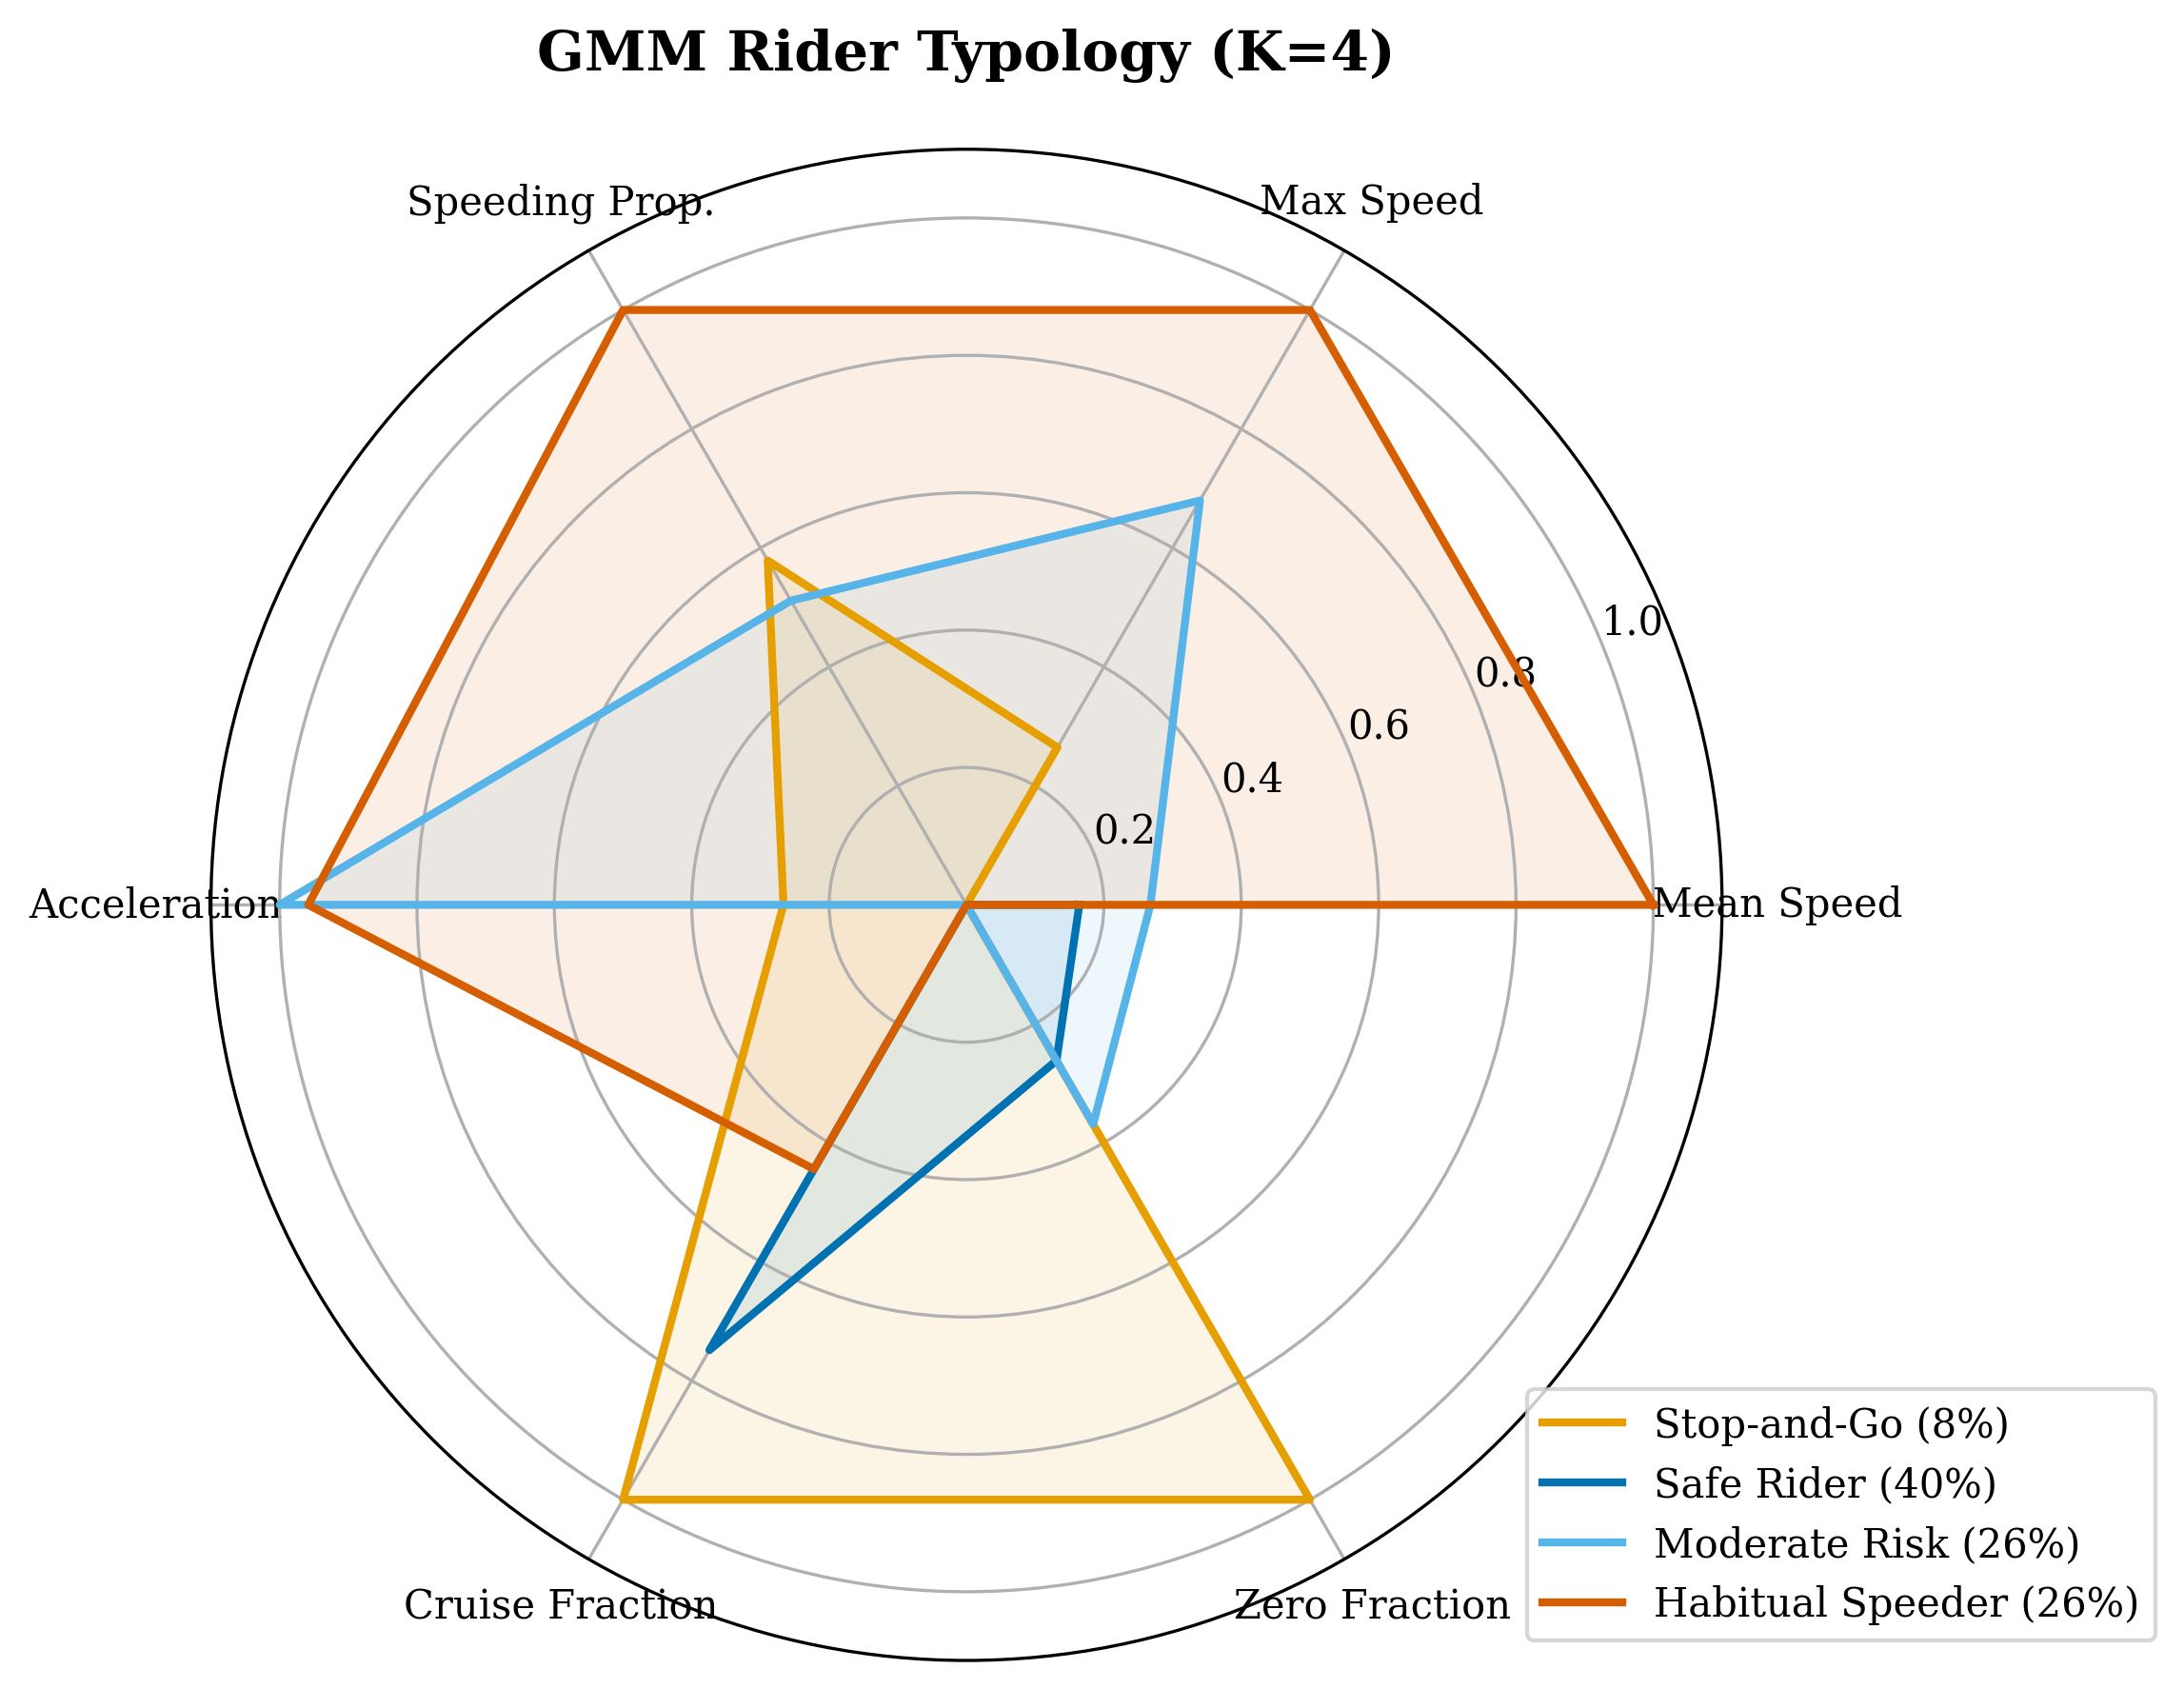
\includegraphics[width=\linewidth,height=0.58\textheight,keepaspectratio]{fig11_rider_typology_radar.png}
  \vspace{-4pt}

  {\scriptsize Safe Rider (40\%), Moderate Risk (26\%), Habitual Speeder (26\%), Stop-and-Go (8\%).}
\end{column}
\begin{column}{0.62\textwidth}
  \centering
  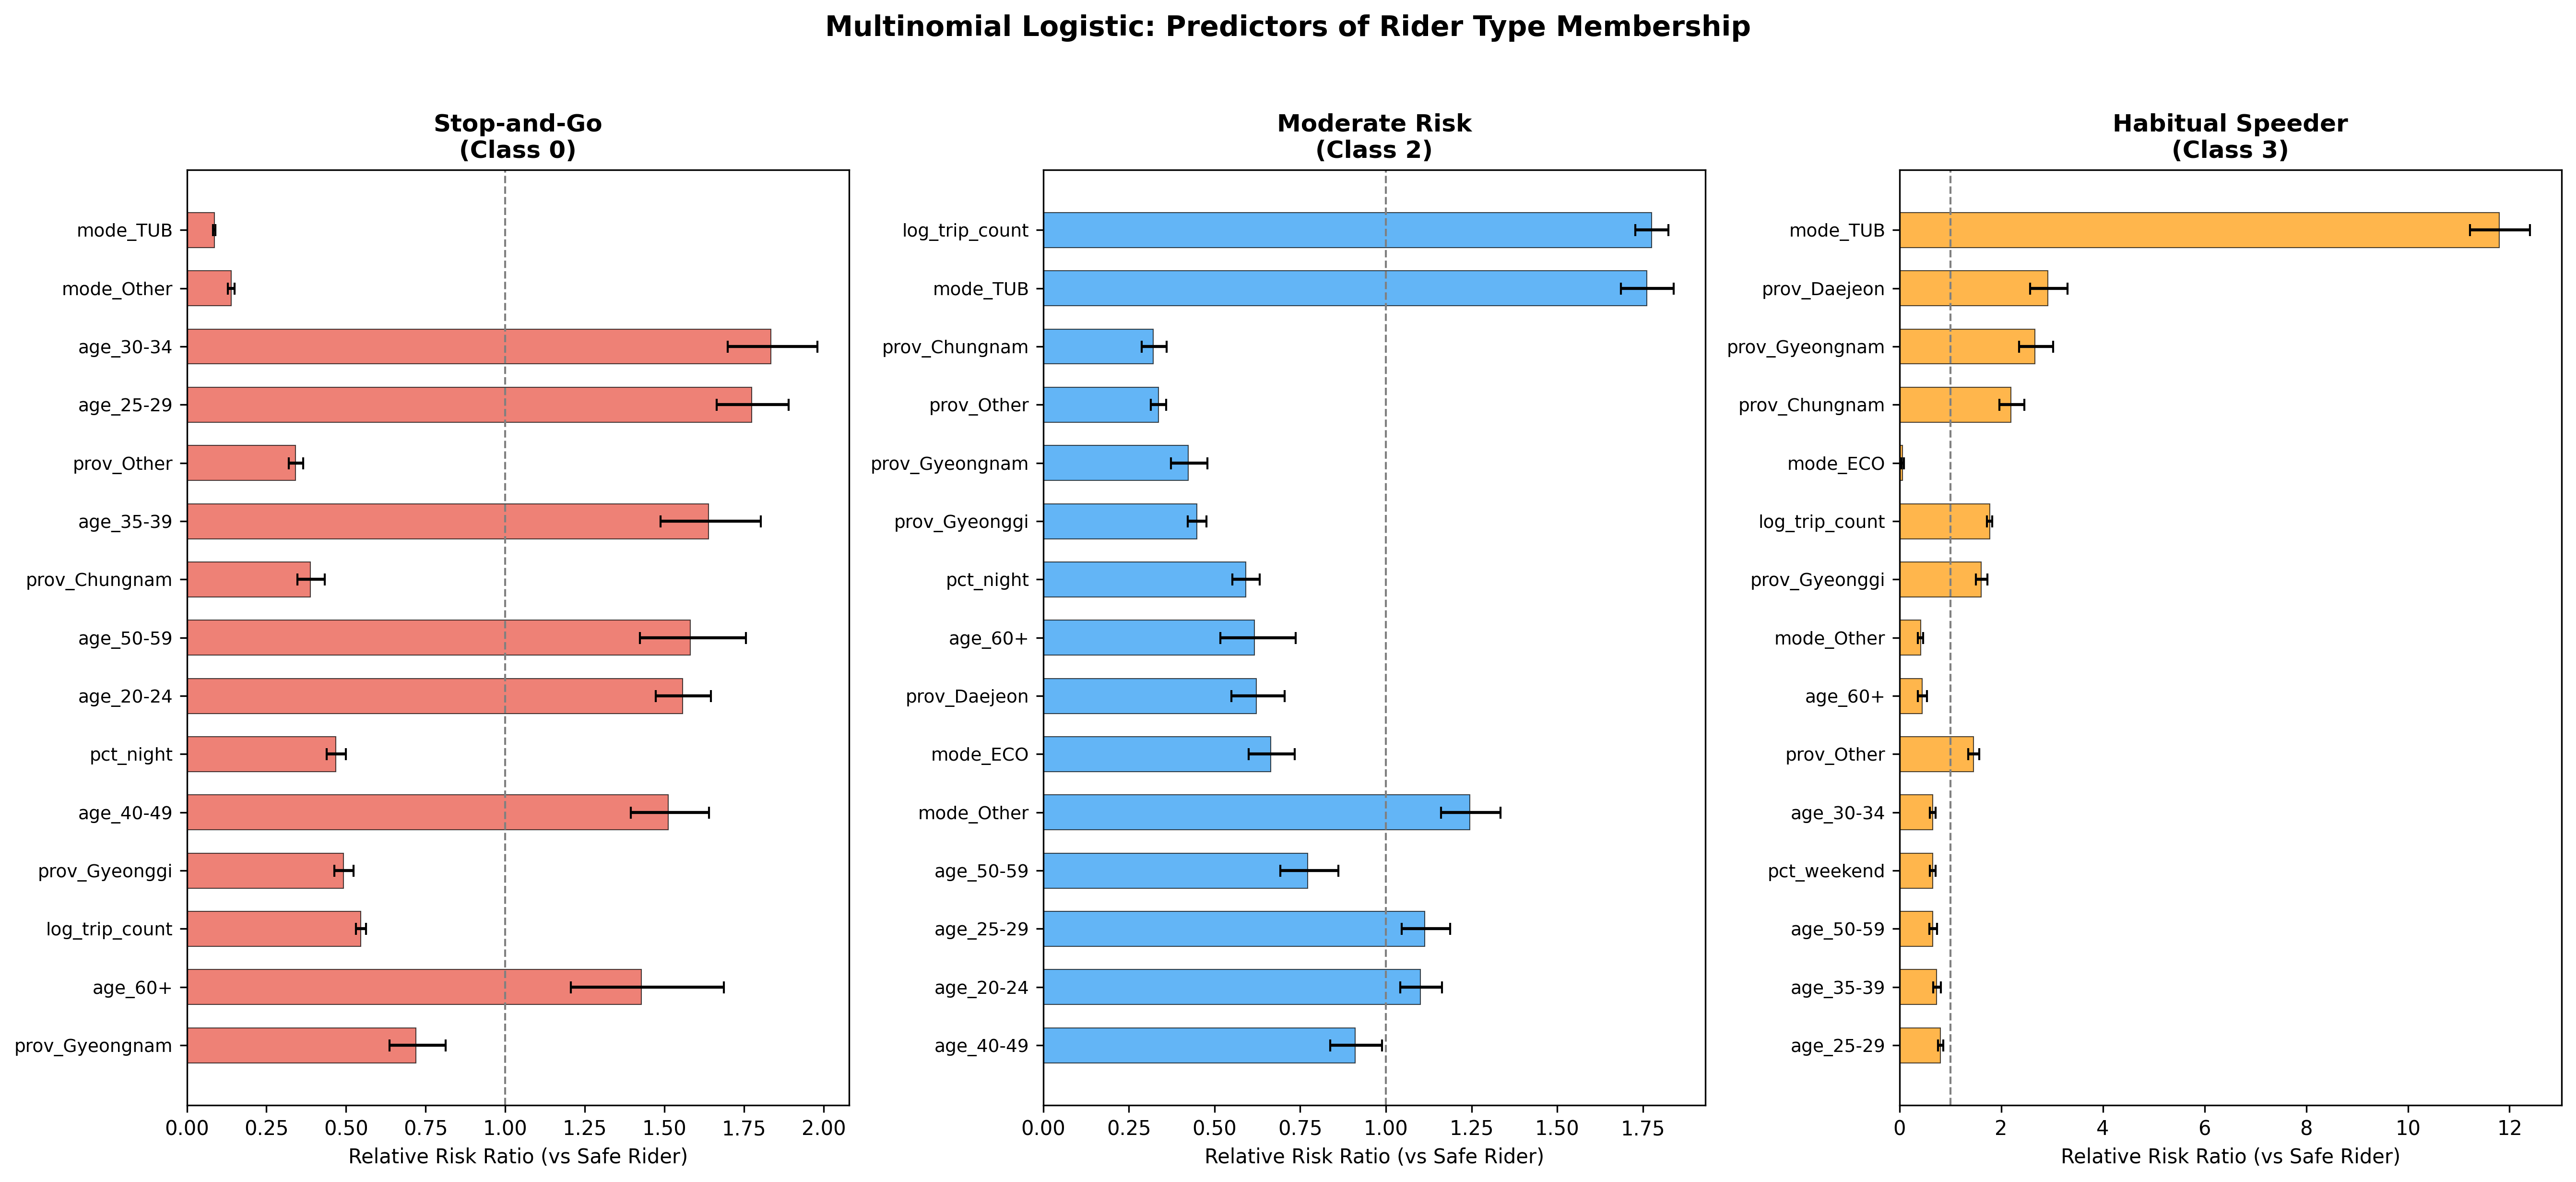
\includegraphics[width=\linewidth,height=0.40\textheight,keepaspectratio]{multinomial_coefficients.png}
  \vspace{-4pt}

  {\scriptsize Multinomial logistic RRR vs.\ Safe Rider. TUB: 11.8 for Habitual Speeder; ECO: 0.06. Pseudo $R^2 = 0.297$.}

  \vspace{2pt}
  \scriptsize\textbf{Key Membership Predictors}
  \begin{itemize}\setlength\itemsep{0pt}
    \item \textbf{TUB mode}: 11.8$\times$ more likely Habitual Speeder
    \item \textbf{ECO mode}: 94\% less likely Habitual Speeder
    \item Daejeon, Gyeongnam: elevated risk
    \item Higher trip count $\to$ Moderate Risk or Habitual Speeder
  \end{itemize}
\end{column}
\end{columns}
\end{frame}

% ═══════════════════════════════════════════════════════════════════════════
% SLIDE 17: ROBUSTNESS & SENSITIVITY
% ═══════════════════════════════════════════════════════════════════════════
\begin{frame}{Robustness \& Sensitivity Analysis}
\begin{columns}[T]
\begin{column}{0.32\textwidth}
  \centering
  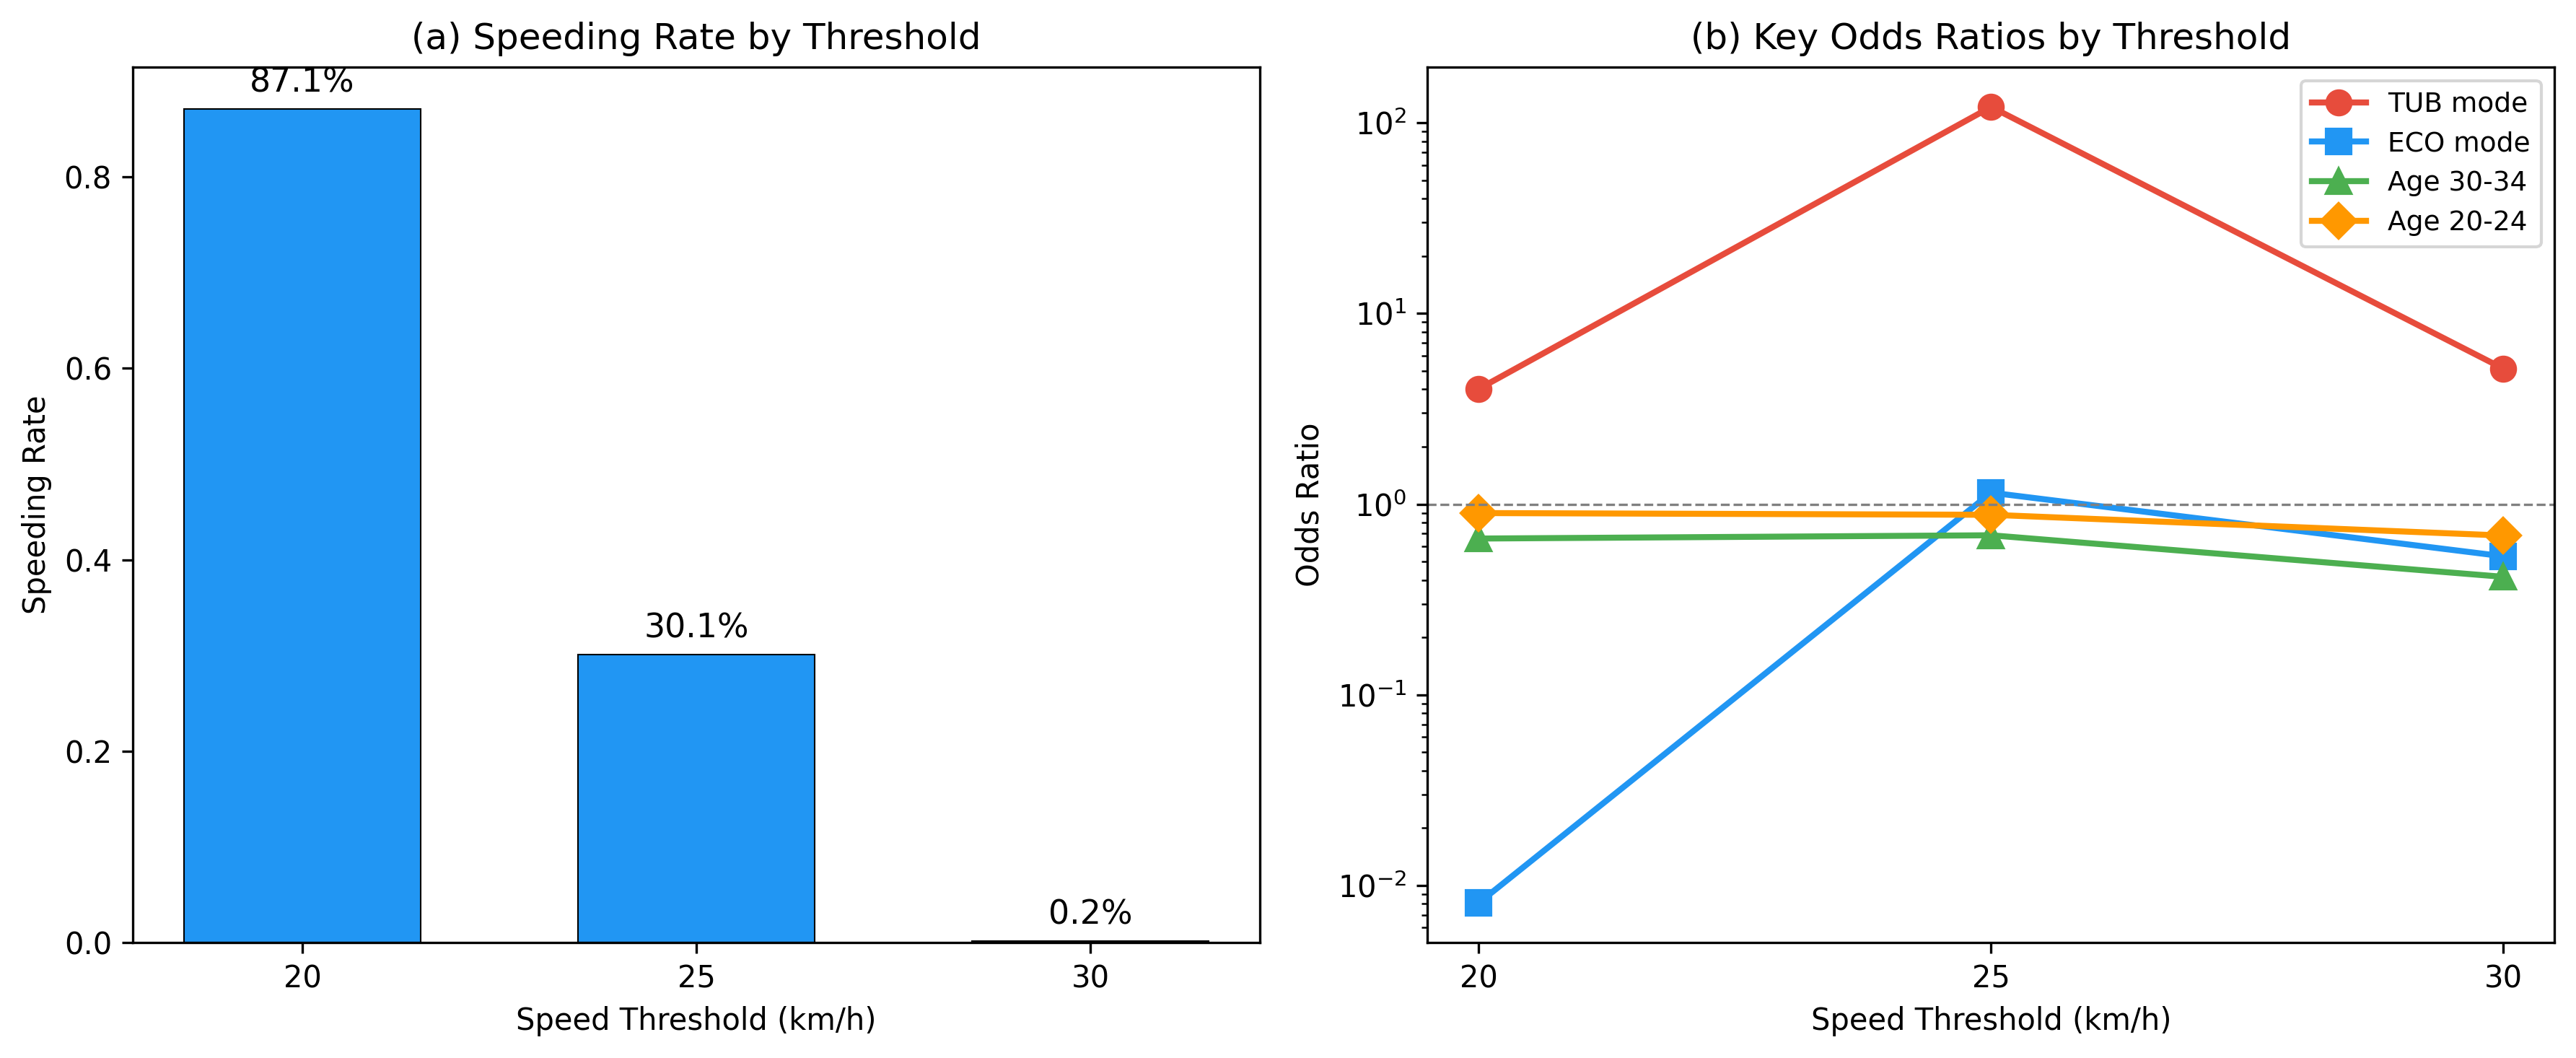
\includegraphics[width=\linewidth]{robustness_threshold.png}
  \vspace{-4pt}

  {\scriptsize \textbf{Threshold:} 20 km/h $\to$ 87\%; 25 $\to$ 30\%; 30 $\to$ 0.2\%. TUB OR peaks at 25 km/h.}
\end{column}
\begin{column}{0.32\textwidth}
  \centering
  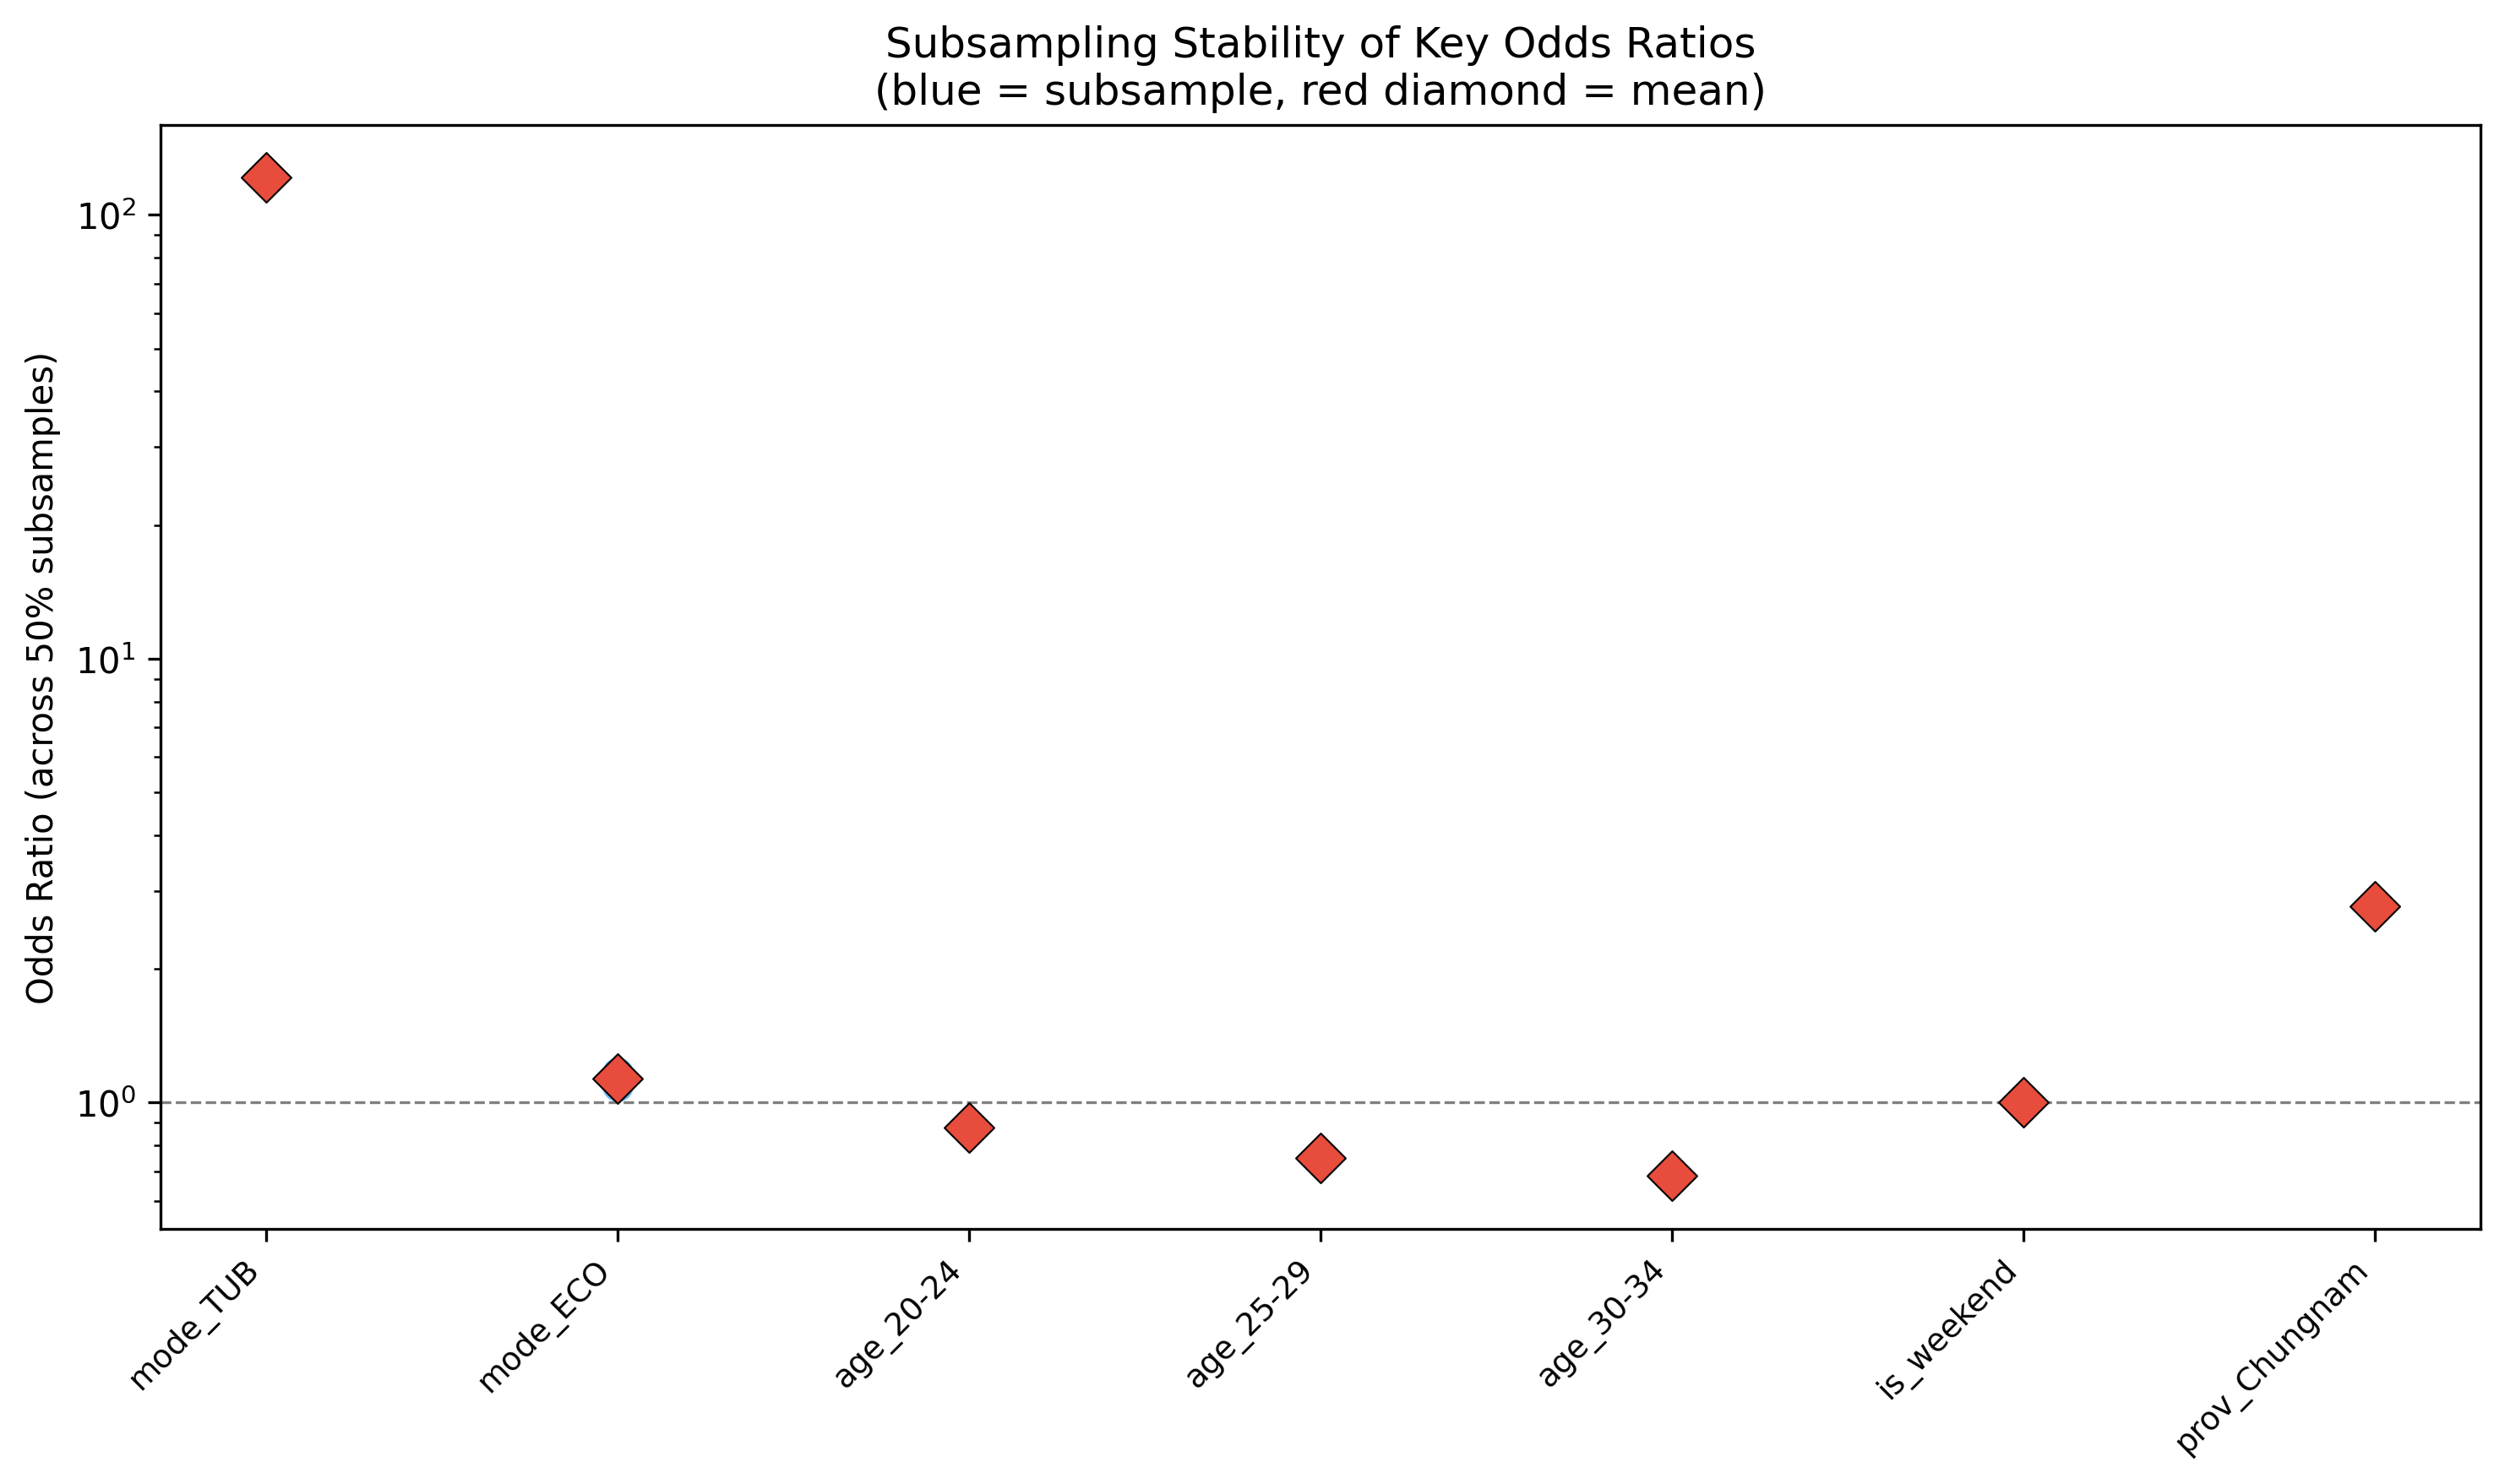
\includegraphics[width=\linewidth]{robustness_subsampling.png}
  \vspace{-4pt}

  {\scriptsize \textbf{Subsampling:} 5$\times$ 50\% samples. TUB OR mean $= 121$, CV $= 1.2\%$.}
\end{column}
\begin{column}{0.34\textwidth}
  \centering
  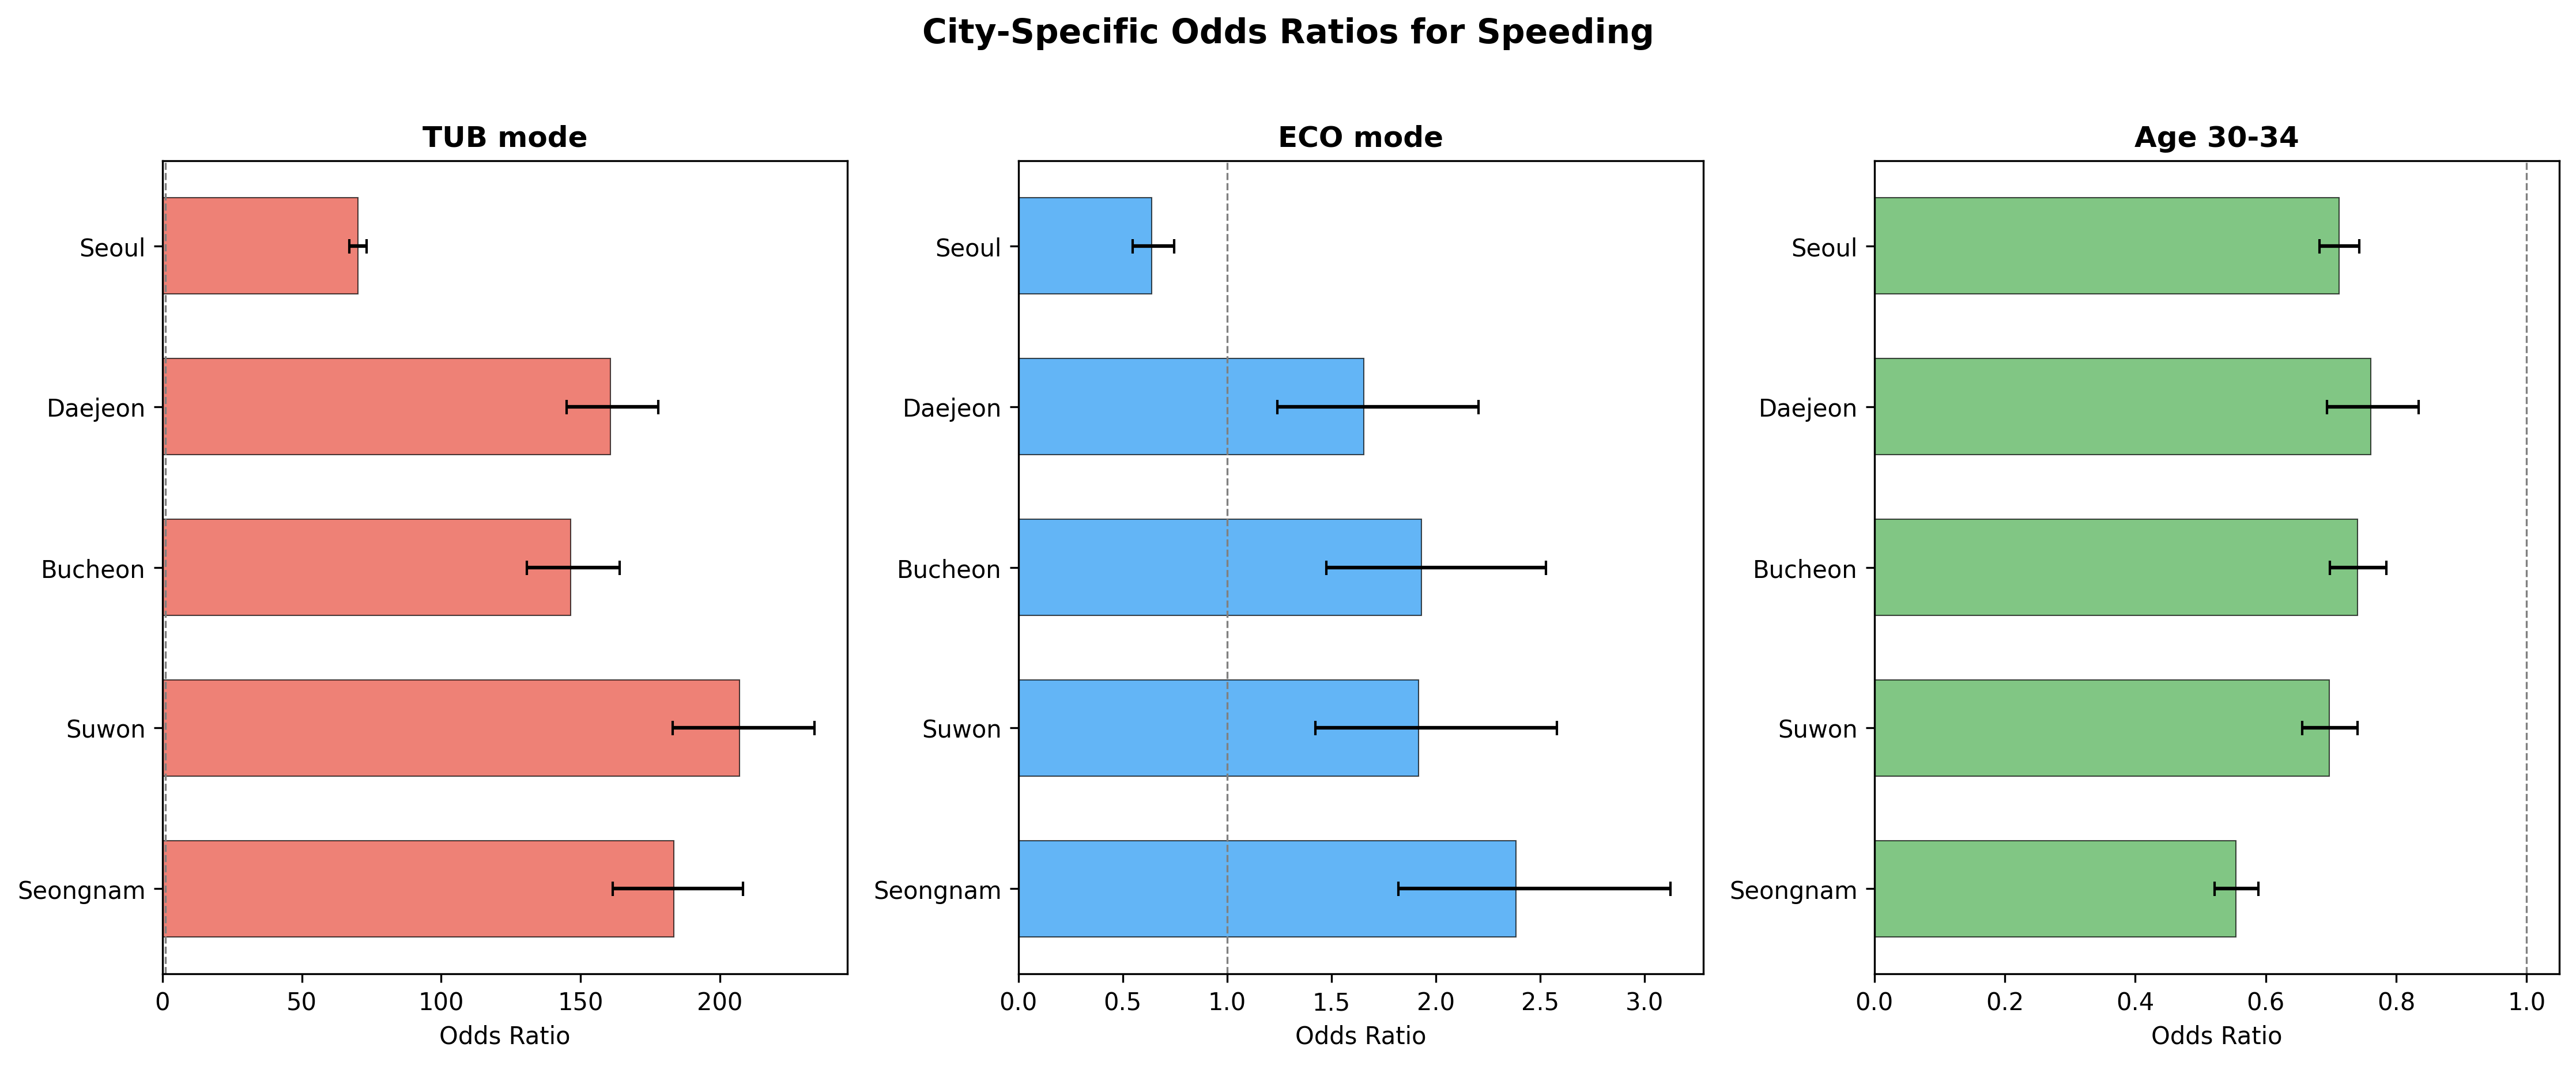
\includegraphics[width=\linewidth]{robustness_city_models.png}
  \vspace{-4pt}

  {\scriptsize \textbf{City-specific:} TUB OR 70--207. ECO \& age effects consistent.}
\end{column}
\end{columns}

\vspace{4pt}
\centering
\scriptsize
\begin{tabular}{@{}l c c c c@{}}
  \toprule
  \textbf{Check} & \textbf{TUB OR} & \textbf{Age 30--34} & \textbf{ECO OR} & \textbf{Stable?} \\
  \midrule
  Full model ($N{=}2.32$M) & 121 & 0.70 & 1.17 & --- \\
  5$\times$ subsampling (CV) & 121 (1.2\%) & 0.70 (0.8\%) & 1.17 (0.5\%) & Yes \\
  City-specific range & 70--207 & 0.54--0.84 & 0.75--2.03 & Yes \\
  Threshold 20 km/h & 3.9 & 0.87 & 0.01 & Direction consistent \\
  Threshold 30 km/h & 0.6 & 0.52 & --- & Partial \\
  \bottomrule
\end{tabular}
\end{frame}

% ═══════════════════════════════════════════════════════════════════════════
% SLIDE 18: CONCLUSIONS & POLICY IMPLICATIONS
% ═══════════════════════════════════════════════════════════════════════════
\begin{frame}{Conclusions \& Policy Implications}
\begin{columns}[T]
\begin{column}{0.47\textwidth}
  \footnotesize
  \textbf{\textcolor{boxbrown}{Answers to Research Questions}}

  \vspace{2pt}
  \textbf{RQ1:} 29.6\% of trips exceed 25 km/h. 60.9\% of users never speed, but 17.3\% speed on $>$50\% of trips.

  \vspace{2pt}
  \textbf{RQ2:} Speeding clusters spatially (Moran's $I{=}0.21$--$0.71$, all $p{<}0.001$). Hot spots have less cycling infra.

  \vspace{2pt}
  \textbf{RQ3:} Mode dominates (TUB OR $= 121$). ECO reduces speeding 54\%$\to$1.1\%. Age 30--34 safest (OR $= 0.70$).

  \vspace{2pt}
  \textbf{RQ4:} Four rider types. 26\% Habitual Speeders, predicted by TUB (RRR $= 11.8$).

  \vspace{4pt}
  \textbf{\textcolor{boxbrown}{Contributions}}
  \begin{itemize}\setlength\itemsep{0pt}\footnotesize
    \item Largest e-scooter speed study (2.83M trips)
    \item Replicable multi-level safety framework
    \item Evidence for data-driven micromobility regulation
  \end{itemize}
\end{column}
\begin{column}{0.50\textwidth}
  \footnotesize
  \textbf{\textcolor{boxbrown}{Policy Recommendations}}

  \vspace{2pt}
  \begin{enumerate}\setlength\itemsep{2pt}\footnotesize
    \item \textbf{Speed governors}: ECO mode virtually eliminates speeding. Mandate as default operating mode.

    \item \textbf{Geofencing}: Deploy dynamic speed limits in identified spatial hot spots (Seoul: 101 hexes).

    \item \textbf{Targeted intervention}: 17.3\% habitual speeders cause disproportionate risk. Progressive penalties.

    \item \textbf{Infrastructure}: Cycling infra associated with lower speeding. Expand protected lanes in hot spot corridors.
  \end{enumerate}

  \vspace{4pt}
  \textbf{\textcolor{boxbrown}{Future Work}}
  \begin{itemize}\setlength\itemsep{0pt}\footnotesize
    \item Link speed behavior to crash data
    \item Real-time safety scoring for dynamic geofencing
    \item Extend to e-bikes and other micromobility
  \end{itemize}
\end{column}
\end{columns}
\end{frame}

\end{document}
